\documentclass[12pt,a4paper,oneside]{book}
\usepackage[a4paper,margin=1in]{geometry}
\usepackage[english]{babel}
\usepackage[utf8]{inputenc}
\usepackage[nottoc]{tocbibind}
\usepackage{amssymb}
\usepackage{hyperref}
\usepackage[nameinlink]{cleveref}
\usepackage{graphicx}
\usepackage{fancyhdr}
\usepackage{multirow}
\usepackage[font=small]{caption}
\usepackage{xcolor}
\usepackage{lscape}
\usepackage{subcaption}
\usepackage{floatrow}
\usepackage{sectsty}
\usepackage[skip=10pt, indent=0pt]{parskip}
\usepackage[explicit]{titlesec}
\usepackage[numbers, sort&compress ]{natbib}
\usepackage{minted}
\usepackage{algorithm}
\usepackage{algpseudocode}
\usepackage{tikz, blindtext}

\definecolor{scarlat}{HTML}{c72125}
\allsectionsfont{\sffamily}
\chapterfont{\sffamily\color{scarlat}}

\pagestyle{fancy}
\fancyhf{}
\fancyfoot[L]{\thepage}
\fancyfoot[R]{\leftmark}
\fancyfoot[C]{}
\renewcommand{\headrulewidth}{0pt}
\renewcommand{\footrulewidth}{0.5pt}
\renewcommand{\chaptermark}[1]{\markboth{#1}{}}

\fancypagestyle{plain}{%
    \fancyhf{}
    \fancyfoot[C]{\thepage}
    \fancyfoot[L,R]{}
    \renewcommand{\headrulewidth}{0pt}
    \renewcommand{\footrulewidth}{0.5pt}
}

\newskip\bigskipamount \bigskipamount =20pt plus 4pt minus 4pt
% \setcounter{tocdepth}{1}
\setcounter{secnumdepth}{3}

\begin{document}
\pagenumbering{roman}

\begin{titlepage}
\centering

\includegraphics[width=0.7\linewidth]{graphics/tue-logo.png}\par
Department of Mathematics and Computer Science

\vspace{3cm}

{\sffamily\LARGE\textbf{
A Study on the Impact of Different Algorithms in Blockchain-based Federated Learning Systems Using a Modular Framework
}}

\par\vspace{2cm}
{\large\textit{Master Thesis}}\\
\vspace{0.2cm}
{\large Henrique Afonso Coelho Dias}

\vspace{2cm}

\textbf{Supervisor} \\
\vspace{0.1cm}
prof. dr. ir. N. Meratnia

\par

\textbf{Assessment Committee} \\
\vspace{0.1cm}
prof. dr. ir. N. Meratnia \\
prof. dr. ir. P.H.F.M. Verhoeven \\
prof. dr. ir. S. Sciancalepore \\

\vfill

{Eindhoven, September 2022}

\end{titlepage}

\chapter*{Abstract}\label{chapter:abstract}
Blockchain-based Federated Learning eliminates the central coordinator of classical Federated Learning networks, allowing multiple distributed clients to cooperate on the same Machine Learning model, without a single point of failure in the network. It is common to score each client's submission in order to determine if it is a good contribution to the global model. With Federated Learning being increasingly adopted in IoT networks, where low powered devices with low resources are the norm, it is important to ensure that certain aspects of the system that can be changed consume the least amount of resources. The current literature has very little information regarding how different aspects impact the system. Additionally, there is no publicly available framework that can be used to implement a Blockchain-based Federated Learning system.

In this thesis, we design and implement the first modular open-source framework for Blockchain-based Federated Learning using Ethereum and TensorFlow. This framework can be easily adapted to support multiple architectures, as well as different scoring, aggregation and privacy techniques. With this framework, we proceed to do the first known analysis of how different aspects of Blockchain-based Federated Learning, such as consensus algorithms, participation selection techniques and scoring techniques, impact the accuracy, execution time and communication and computation costs. Additionally, the same analysis is done per each scoring technique regarding the impact of the number of clients and privacy techniques. Finally, we also provide a proof of concept of how the framework can be adapted to support, not only Horizontal Federated Learning, but also Vertical Federated Learning.

\tableofcontents

\listoffigures

\listoftables

\chapter{Introduction}\label{chapter:introduction}
\pagenumbering{arabic}
Machine Learning (ML) has revolutionized the way we use and work with data, opening ways to new techniques and explorations. ML models can be powerful tools to predict things that would otherwise require high amounts of human effort. For example, an image recognition model may be created to help medical professionals diagnose diseases. Similarly, a model may be created to detect abnormal heart rate or walking patterns based on smart watch sensor data. Even though models such as these can be very helpful, they have to be trained with high amounts of good quality data in order for the model to perform accurately \cite{10.1145/3394486.3406477}. To address this issues, there are techniques that allow multiple parties to collaboratively train the same models.

In 2016, Google researchers attempted to build communication-efficient deep neural networks in decentralized settings \cite{10.48550/arxiv.1602.05629}. The result of this work was the introduction of a new way of collaboratively training Machine Learning models, which they termed Federated Learning. Federated Learning (FL) allows multiple clients, in different locations, to collaborate on the training of a global Machine Learning model without sharing their own data with each other. Instead of sharing the raw data, clients only share model parameters, such as weights. This brings some benefits. The first benefit is that, by not sharing raw data, models can preserve data privacy, allowing them to be trained on sensitive data. In addition, since model parameters are usually much smaller than the raw data, this leads to less data being transported over the networks. Finally, since the data is distributed among different clients, a single powerful server is not required to train the model, as usually training models with smaller amounts of data is less computationally expensive.

\section{Motivation}\label{intro:motivation}

Currently, most FL networks include a central server that coordinates the federated training process and aggregates the model weights from each of the clients into a single model. This central coordinator is a single point of failure in the network, since it is always required to be online and behave correctly \cite{li_blockchain_2021, 10.48550/arxiv.2110.02182}. To address this, Blockchain-based Federated Learning (BFL) techniques have been proposed.

By combining Blockchain to Federated Learning, not only can the central orchestrator be eliminated, but also the federated training process can be made more transparent. In the blockchain, each transaction is recorded in the distributed ledger. These transactions record information such as local updates, scores, aggregations, among others. Having this information in a public ledger allows for a transparent training process and reward distribution \cite{li_blockchain_2021}. The following are some aspects that Blockchain can bring to Federated Learning when combined:

\begin{itemize}
    \item \textit{Traceability and Auditability}. Due to the structure of the blockchain, it is possible to trace transactions to their original source, which can be useful for auditability purposes \cite{10.48550/arxiv.1902.01046, 10.48550/arxiv.2110.02182}.
    
    \item \textit{Data Immutability and Persistency}. Once transactions are added to the distributed ledger, it is nearly impossible to revert them or change their information \cite{10.48550/arxiv.1902.01046, qu_blockchain-enabled_2022}. This ensures that data is not changed and it can be retrieved after the fact.
    
    \item \textit{Decentralization}. The involvement of a central orchestrator is eliminated and the processing of the aggregation is replaced by multiple servers \cite{10.48550/arxiv.2009.09338, 9403374, 10.48550/arxiv.2110.02182, qu_blockchain-enabled_2022}. This improves the resilience and availability of the system.
    
    \item \textit{Authentication}. Blockchain ensures the authentication of data and messages due to the verification mechanisms in place, such as the usage of private keys to sign transactions \cite{qu_blockchain-enabled_2022}.
\end{itemize}

Blockchain platforms can implement different consensus algorithms, which can lead to very different resource consumption \cite{ccaf}, as well as different degrees of latency \cite{Alqahtani_2021}. Two other important aspects in BFL systems are the participant selection and the scoring algorithms. While the former indicates how the participants are chosen to submit their updates in each round, the latter aids on scoring each client's model update in order to identify which ones are the best and should be included in the final aggregation. All this algorithms influence the accuracy, convergence, and resource consumption. At the same time, each algorithm performs differently with different amounts of devices, as well as with different degrees of privacy, leading to different accuracy results, as well as resource consumption.

\section{Problem Statement}\label{intro:problem}

To the best of our knowledge, there is very little literature on the impact of different algorithms of BFL systems, namely consensus, participant selection and scoring algorithms, on the execution time, accuracy, convergence, communication and computation costs of the system. In addition, there is no research on how different scoring algorithms are impacted in terms of the aforementioned aspects when different amounts of clients and privacy degrees are used. With BFL being increasingly adopted in IoT networks, where low powered devices with low resources are the norm, it is important to ensure the system consumes the least amount of resources, especially regarding the clients.

Additionally, even though there is literature on designing BFL frameworks, none of them are open source, or modular enough to support different algorithms. Such framework could be used to empower future research on new algorithms, as well as help those who want to implement their own BFL system.

\section{Research Questions}\label{intro:questions}

Taking into account the motivation and problem statement, this work will focus on answering the following main research question:

\begin{center}
    \textit{What is the impact of different consensus, participant selection and scoring algorithms in a Blockchain-based Federated Learning system on execution time, convergence and accuracy, as well as communication and computation costs?}
\end{center}

This research question can be further sub-divided into four sub-questions:

\begin{enumerate}
    \item \textit{How to design a modular framework that allows easy customization of different algorithms related to different parts of the Blockchain-based Federated Learning system?}
    
    \item \textit{How do consensus, participant selection, and scoring algorithms influence execution time, convergence, accuracy, and communication and computation costs of the system?}
    
    \item \textit{How does the number of clients, as well as degrees of privacy impact the different scoring algorithms?}
    
    \item \textit{How can we build a Blockchain-based Federated Learning framework that supports different data partition formats, such as vertical and horizontal?}
\end{enumerate}

\section{Contributions and Outline}\label{intro:outline}

The contributions of this thesis are as follows: (i) design and implementation of the first open-source modular framework for BFL that can be easily adapted to support new scoring, aggregation, and privacy algorithms. This framework can be used to empower future research; (ii) the first comparative study of how different algorithms of BFL, namely consensus, participant selection, and scoring algorithms, impact the execution time, transaction costs, transaction latency, model accuracy and convergence, communication costs, and computation costs of the system; (iii) the first comparative study of how the number of clients and different degrees of privacy impact the accuracy, execution time and communication and computation costs of different scoring algorithms; and (iv) a proof-of-concept of a Blockchain-based Vertical Federated Learning.

The remainder of the thesis is structured as follows. \Cref{chapter:background} provides definitions and fundamental concepts about BFL, as well as background information of the algorithms and mechanisms that will be explored. \Cref{chapter:related_work} reviews the existing work regarding algorithms and mechanisms used in BFL systems. \Cref{chapter:framework} explains the design and implementation of the framework. \Cref{chapter:evaluation} provides information regarding the experimental setup of the experiments. \Cref{chapter:analysis:consensus_algorithms} provides the impact analysis of using different consensus algorithms. \Cref{chapter:horizontal} provides the impact analysis of using different scoring algorithms, as well as how they behave with different number of clients and privacy degrees. \Cref{chapter:vertical} provides analysis of the proof of concept of Vertical Federated Learning applied in a BFL system. Finally, \Cref{chapter:conclusion} discusses the results, contributions and provides directions for future works.



\chapter{Background}\label{chapter:background}
This chapter gives an overview of the fundamental concepts and the algorithms important for this thesis.

\section{Machine Learning}\label{background:machine_learning}

Machine Learning is a sub-field of Artificial Intelligence that builds models based on statistical and algorithmic concepts in order to detect relevant patterns based on previously-seen data \cite{geron_2019}. There are four categories of learning, i.e., \textit{supervised}, \textit{semi-supervised}, \textit{unsupervised} and \textit{reinforcement learning} \cite{Sarker2021}. Each category performs different types of tasks on different types of data. This study focuses only on supervised learning.

In supervised learning, algorithms build mathematical models from labeled data, which is data in the format $(X, y)$, where $X$ is the input sample and $y$ is the expected output, or label. During training, algorithms provide the model with the input samples and improve the model by comparing its output with the expected outputs (the so called ground truth). Supervised learning problems can be divided into \textit{regression problems}, if the output is a continuous variable, or \textit{classification problems}, if the output is a discreet variable \cite{Sarker2021}.

\subsection{Federated Learning}\label{background:federated_learning}

Federated Learning is a ML technique, in which different distributed clients collaboratively train a model under the supervision of a centralized server. Clients are distributed heterogeneous devices with their own computing resources and they are responsible for producing and maintaining their own data \cite{9084352}. The data is assumed to be non independent or non identically distributed (\textit{non-iid}).

Since clients are heterogeneous and distributed, having different communication costs and response times are normal. In addition, some clients may operate under constrained networks with either low or limited bandwidth. Therefore, it is important that new FL techniques ensure that communication and resource usage is minimized.

During the training process, the raw data never leaves the clients and only the model parameters, such as model weights, are exchanged with the server in order to compute the global model. However, model weights can be target of inference attacks and leak secret information \cite{10.1145/3298981}.  Consequently, new Federated Learning architectures and algorithms must be compatible with techniques that guarantee privacy, such as differential privacy, homomorphic encryption, secure multiparty computation or other cryptographic protocols \cite{10.1145/3298981}.

After each round of training, the central server aggregates the local updates. Usually, this is done using a mathematical formula, for example, Federated Averaging (\textit{FedAvg}) \cite{10.48550/arxiv.1602.05629}, which calculates the weighted average of all clients.
% $k \in K$ weights $w^k$:

% \begin{equation}
% w_{t+1} = \sum_{k \in K} \frac{n_k}{n} w_{t+1}^k
% \end{equation} \label{eq:fedavg}

% Where $n_k$ is the number of samples that the client $k$ used to train and $w_{t+1}^k$ the weights of client $k$ at round $t+1$.

\subsection{Categories of Federated Learning}\label{background:archfl}

According to \cite{10.1145/3298981, 10.1145/3412357}, with respect to the different data partition among the clients, the federated Learning techniques can be broadly divided into three main categories, i.e., (i) 
horizontal, (ii) vertical, and (iii) federated Transfer Learning. We focus on the first two categories.

In \textit{Horizontal Federated Learning} (HFL), clients with the same data structure collaborate to build a single model. In other words, the different data sets in the different clients share the same feature space, but not the sample space. For example, two banks branches operating in different cities have similar businesses (feature space), but different clients (sample space). The architecture of HFL, depicted in \autoref{fig:hfl_arch}, consists of multiple clients training a model, while the central server performs the aggregation of all local updates.

In \textit{Vertical Federated Learning} (VFL), clients share an intersecting sample space, but different feature spaces. For example, two different banks with different products operating in the same city have a similar client base (sample space), but different information about each client (feature space). The architecture of VFL, depicted in \autoref{fig:vfl_arch}, is similar to the one of HFL. However, it requires an additional step, calculating the Private Set Intersection (PSI) \cite{wei2022vertical}, since the clients do not share the exact same sample space. PSI is a protocol by which multiple clients can calculate the common samples without sharing their raw data \cite{wei2022vertical}.

\begin{figure}[!htp]
    \centering
    \centering
    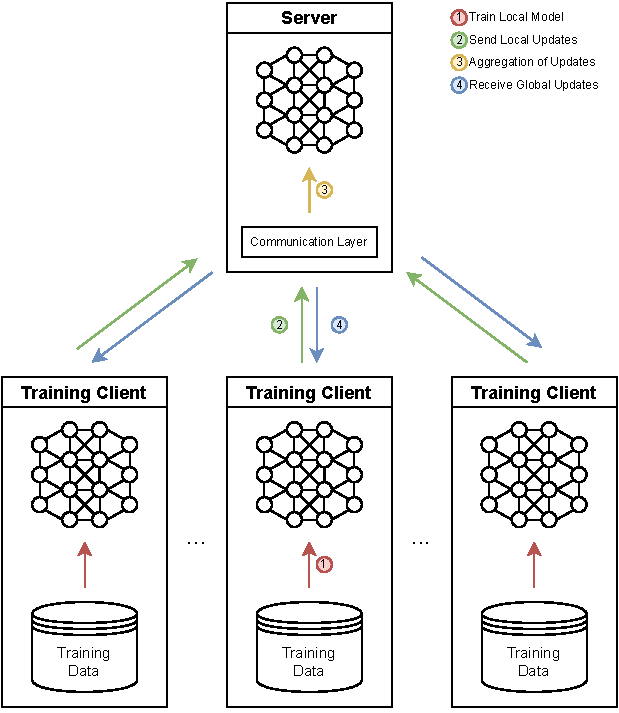
\includegraphics[width=0.6\textwidth]{graphics/hfl-architecture.pdf}
    \caption{Horizontal Federated Learning Architecture}
    \label{fig:hfl_arch}
\end{figure}

\begin{figure}[!hbp]
    \centering
    \centering
    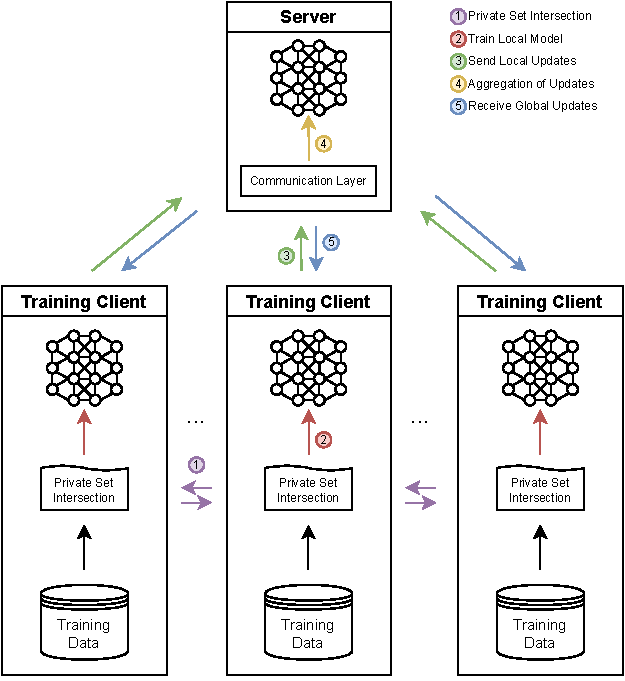
\includegraphics[width=0.6\textwidth]{graphics/vfl-architecture.pdf}
    \caption{Vertical Federated Learning Architecture}
    \label{fig:vfl_arch}
\end{figure}

\section{Blockchain}\label{background:blockchain}

A blockchain is an immutable distributed ledger, which is a database of transactions maintained by several computers, also known as nodes, linked through a peer-to-peer network. The concept of blockchain was first introduced by Stuart Haber and W. Scott Stornetta in 1991 \cite{10.48550/ARXIV.1810.06130}, being popularized by Satoshi Nakamoto in 2008 with the introduction of the cryptocurrency Bitcoin \cite{nakamoto2009bitcoin}.

\begin{figure}[h]
    \centering
    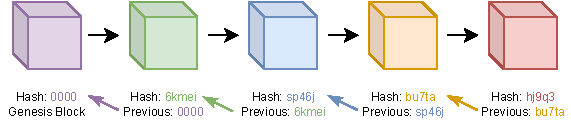
\includegraphics[width=0.8\textwidth]{graphics/blockchain.pdf}
    \caption{Blockchain Representation}
    \label{fig:blockchain_blocks}
\end{figure}

In a blockchain, the data is structured as blocks, as can be seen in \autoref{fig:blockchain_blocks}. Each block contains a certain number of transactions and links to the previous block via a cryptographic hash, forming a chain. This guarantees fidelity and trust without requiring a trusted third party, which is why it is called a \textit{trustless} system. In addition, since the record is immutable and decentralized, all transactions can be transparently viewed by others.

As mentioned beforehand, a blockchain is maintained by several nodes in a peer-to-peer network. As transactions come in, nodes compete in order to generate the next block. Since it is a decentralized process, multiple nodes will try to create the next block of the chain in parallel. In order to reach an agreement between the nodes, a consensus algorithm is used. The consensus algorithm allows to reach an agreement between multiple decentralized nodes without requiring a singular node to be in charge.

\begin{figure}[h]
    \centering
    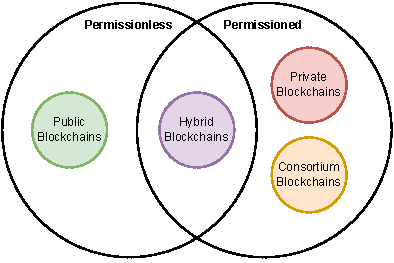
\includegraphics[width=0.5\textwidth]{graphics/blockchain-types.pdf}
    \caption{Blockchain Types}
    \label{fig:blockchain_types}
\end{figure}

\autoref{fig:blockchain_types} illustrates four different types of blockchain, i.e., public, private, consortium, and hybrid. Some are permissionless, which means that anyone can join the network, while some are permissioned, which means that only allowed parties can join the network. 

\begin{itemize}
    \item \textit{Public Blockchains} are permissionless and therefore anyone can join and participate in the network. There is no central authority.

    \item \textit{Private Blockchains}, in contrary to the public blockchains, private blockchains are permissioned with a single central authority. They can only be accessed by allowed parties and they are usually used within organizations.

    \item \textit{Consortium Blockchains}, similarly to the private blockchains, are permissioned. However, instead of being controlled by a single authority, they are controlled by a group of different authorities.

    \item \textit{Hybrid Blockchains} have features of both permissioned and permissionless blockchain systems. They, on one hand, are usually controlled by a single authority, while on the other hand, have a mixed usage of permissioned and permissionless protocols running in parallel for different use cases.
\end{itemize}

\subsection{Smart Contracts}\label{background:smart_contracts}

Smart contracts \cite{8500488} are small computer programs that live within the blockchain and automatically run when predetermined conditions are met. As they live in the blockchain, they are trustless and are typically used to automate the execution of agreements. This way, every party involved in the agreement is certain that it will be honored once the conditions of the agreement are met. Some blockchain platforms, such as the Ethereum \cite{wood2014ethereum}, provide functionality for smart contracts.

\subsection{Blockchain Platforms}\label{background:blockchain_platforms}
 
As explained in \autoref{background:blockchain}, blockchain platforms allow developers to build applications on top of the blockchain technologies. Even though all platforms are based on the concept of blockchain, they all have different characteristics and restrictions, as well as different sets of features.

As it can be seen in \autoref{tab:platf_consensus}, around half of the implementations used an already existing platform, where the remaining preferred to implement their own blockchain platform. Among already existing platforms, Ethereum is the most popular. When implementing a custom platform, it is easier to overcome certain restrictions such as limits on data per block \cite{8733825, 9524833}.

\subsection{Consensus Algorithm}\label{background:consensus_algorithms}

The consensus algorithm is one of the most important components of a Blockchain platform. Consensus is the process of reaching an agreement on a single value among different distributed processes \cite{9347812}. These algorithms are designed to be reliable even on networks that have unreliable blockchain nodes. In blockchain, the consensus algorithm is used to reach consensus on the next block of the chain \cite{9079513}. The following consensus algorithms will be compared in our work:

\begin{itemize}
    \item The \textit{Proof of Work (PoW)} \cite{finney} consensus algorithm was first introduced in the context of blockchain platforms by Satoshi Nakamoto in Bitcoin \cite{nakamoto2009bitcoin}. It works by means of computation effort proofs, where a set of virtual miners race in solving a complex, yet feasible, mathematical problem. The winner of the race generates a cryptographic proof based on the solution of the problem that can be easily verified by others. Then, the winner adds a new block containing the newly verified transactions to the blockchain. In addition, the winner is rewarded according to some pre-determined rules.
    
    On the one hand, it is a simple algorithm, for which proofs are hard to create, but easy to verify \cite{li_blockchain_2021}. Not only is it robust and proven to work, but the cost of attacking a PoW blockchain is extremely high \cite{li_blockchain_2021}. For an attack to be successful, it needs to control more than half of the network \cite{li_blockchain_2021}. On the other hand, PoW consumes extreme amounts of energy and it is hard to scale \cite{edwood_2020, li_blockchain_2021, ccaf}.
    
    \item The \textit{Proof of Authority (PoA)} \cite{szilagyi_2017} consensus algorithm is a reputation-based consensus algorithm that is most commonly used in private blockchain networks. It works by having a set of validator nodes that are responsible for validating new transactions. In order to ensure the correctness of the validator nodes, they have to stake their own reputation. In addition, the validators are known trusted entities that are manually chosen by the network owner.
    
    On the one hand, PoA provides high throughput and high scalability \cite{bPoA}. On the other hand, the main criticism of PoA is that it is usually has a small number of validators, that are manually chosen. Therefore, it has a lesser degree of decentralization. Consequently, PoA is not as common in public blockchain networks as it is for private networks \cite{bPoA}.

    \item The \textit{QBFT Byzantine Fault Tolerance (QBFT)} \cite{10.48550/arxiv.2002.03613} consensus algorithm is similar to the Practical Byzantine Fault Tolerance (PBFT) \cite{Castro99practicalbyzantine} algorithm, which is a three-phase protocol that allows a network with $3f+1$ nodes, where $f$ is the maximum amount of faulty nodes, to reach consensus. The different between QBFT and PBFT is that in the former the set of validators is dynamic, while in the latter, it is static. The network reaches a consensus once $2f+1$ nodes agree.
    
    One the one hand, QBFT allows for high consensus efficiency in high throughput networks \cite{li_blockchain_2021}. On the other hand, it will stop working properly if only 33\% or less blockchain nodes are running and it can also have high communication costs due to its three-phase protocol nature \cite{li_blockchain_2021}.
\end{itemize}

\section{Blockchain-based Federated Learning}\label{background:bfl}

Recently, the idea of applying blockchain to FL has emerged. This is motivated by the fact that FL architectures are highly dependent on a single central server, leading to a central point of failure, that can be either overloaded or compromised. With blockchain, the central server can be replaced by multiple decentralized servers that operate the blockchain nodes. In addition, blockchain can provide authentication, traceability, auditability and data preservation.

As stated in \cite{10.48550/arxiv.2110.02182}, so far three different main architecture groups have been proposed for BFL systems: \textit{Fully Coupled BFL}, \textit{Flexibly Coupled BFL}, and \textit{Loosely Coupled BFL}. In Fully Coupled BFL, the distributed clients are the only devices in the network and act as both clients and servers, performing the training and aggregation, as well as running the blockchain nodes. In Loosely Coupled BFL, the central server still exists and blockchain is only used to manage the reputation of clients. Flexibly Coupled BFL provides a middle ground between both, where there are servers and clients in the network. The servers are responsible for maintaining the blockchain nodes and use the blockchain to store information such as aggregations, scores, among others. The architecture is depicted in \autoref{fig:bfl_arch}.

\begin{figure}[!ht]
    \centering
    \centering
    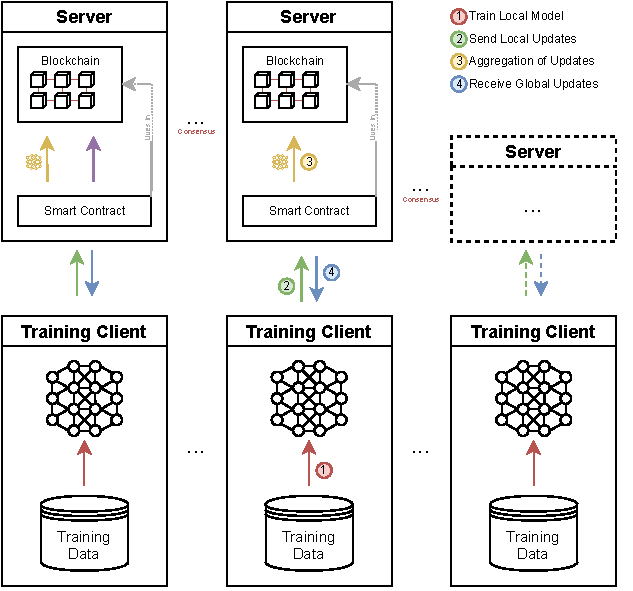
\includegraphics[width=0.6\textwidth]{graphics/bfl-architecture.pdf}
    \caption{Blockchain-based Federated Learning Architecture}
    \label{fig:bfl_arch}
\end{figure}



\subsection{Participants Selection Algorithms}

Participant selection algorithms are algorithms that are used to decide how many and which clients are selected to participate in each round. There are two main participant selection algorithms:

\begin{itemize}
    \item \textit{Random selection}, where both the number of participants, as well as the participants themselves are selected randomly before the start of each round.
    
    \item \textit{First-come first-served}, where the number of participants $n$ is chosen randomly before the start of each round. Then, the first $n$ clients to take initiative to join the round will participate.
\end{itemize}

\subsection{Scoring and Aggregation Algorithms}
\label{background:scoring}

During the training process, each client produces its model parameter updates and communicates them to the servers through the blockchain. These parameters are then aggregated. However, there are different security aspects that should be taken into account here as the parameter updates creates a possibility for performing different attacks such as poisoning attacks \cite{9134967} and plagiarism attacks \cite{10.48550/arxiv.2009.09338}.

\begin{itemize}
    \item \textit{Poisoning attacks} happen when clients willingly send parameter updates that decrease the quality of the model. They may have been generated using an unreliable data set, or done on purpose. To avoid other participants to provide unreliable data to degrade the model performance, there are dynamic verification techniques \cite{10.48550/arxiv.2110.02182, 10.48550/arxiv.2104.10501} that allow to ignore low quality data.
    
    \item \textit{Plagiarism attacks} happen when lazy clients plagiarize other client's models updates without really training their models. These attacks can be addressed via pseudo-noise algorithms \cite{9403374}. In addition, plagiarism attacks within the same round can be avoided by secure communication methods, such as differential privacy \cite{10.48550/arxiv.2009.09338}, through which plagiarism attacks where a client reuses parameters from a previous round can be avoided by simply comparing the different client's updates.
\end{itemize}

To mitigate the poisoning and plagiarism attacks, different scoring algorithms were developed. Scoring algorithms are used to give each client, or its model update, a score. Based on this score, the submission may have more or less impact on the aggregation, if any at all. In addition, scores are used for reward mechanisms in systems where public models are being trained and clients need some sort of incentive to keep participating \cite{8945913, 8832210, 8905038, 9006344}. In this section, we explain briefly how each of the scoring algorithms works and if they influence the aggregation algorithm.

\subsubsection{BlockFlow Score}

The BlockFlow algorithm \cite{10.48550/arxiv.2007.03856} work by giving each submission a score and, based on that score, do the aggregation. In this algorithm, each client $a$ gives each other client $k$ a score $s_{a,k} \in [0.0, 1.0]$, which can be based on $a$'s validation set accuracy using $k$'s submission. Based on this scores, a median score and an evaluation quality scores are calculated. The overall scores will then be the minimum between the scaled median score and the scaled least accurate evaluation score.

With the final scores, the aggregation is calculated using the scores as weights in the Federated Averaging algorithm, instead of the number of samples. More details regarding the algorithm specifics can be found in the original paper.

\subsubsection{Marginal Gain Score}

The Marginal Gain algorithm \cite{10.48550/arxiv.2011.07516}, also known as contributivity score, is calculated by summing the marginal performance gains of all the client's model updates so far. Similarly to BlockFlow scoring, each client has to give each other clients' submission a score. The formula of the client $c$'s submission score $S(c)$ is calculated as follows:

\begin{equation}
    \label{eq:marginal-gain}
    S(c)= \sum_r(v(M_r)-v(M^c_{r+1}))
\end{equation}
, where $v$ is a performance metric, such as accuracy, and $m$ is the model and $r$ the round. These scores are used as weights in the Federated Averaging Algorithm. If the submission's score is equal or below $0$, the submission is ignored.

\subsubsection{Multi-KRUM Score}

The Multi-KRUM algorithm \cite{9170559, Peyvandi2022, 9292450} works by giving each submission a score and eliminating dubious submissions based on their score. This scores are calculated by the servers and are based on the Euclidean distances between the different client $c$'s submissions. The score of each client is denoted as $S(c)$ and calculated as follows:

\begin{equation}
    \label{eq:multi-krum}
    S(c)=\sum_{c \rightarrow k} || \Delta w_c - \Delta w_k|| ^2
\end{equation}

, where $\Delta w$ is a submission and $c \rightarrow k$ are the clients $k$ whose submission $\Delta w_k$ are the $R-f-2$ closest to $\Delta w_c$. In this formula, $R$ is the total number of submissions, while $f$ represents the amount of Byzantine clients. After giving each submission a score, the $R-f$ clients with the lowest scores are chosen and the remaining are rejected. Please note that Byzantine fault tolerant systems behave correctly when no more than $f$ out of $3f+1$ replicas fail.

\subsection{Privacy Mechanisms}

Even though FL is already more secure than centralized ML in the sense that the raw data is never shared, the model weights can be exploited via inference attacks \cite{10.1145/3298981}. Inference attacks are attacks in which the weights are used to reverse-engineer the original data.

Additionally, in BFS systems, the weights are visible to all other client or participant since the blockchain provides an immutable, traceable and auditable record of the whole process. Consequently, it is important to reduce the surface for attacks when it comes to the model parameters.

\subsubsection{(Local) Differential Privacy}\label{background:diff_priv}

Differential Privacy (DP) \cite{hvdiffpriv} is a set of mathematical constrains that algorithms must observe in order to ensure a certain degree of privacy. In other words, some data is differentially private if, by looking at it, we cannot retrieve identifiable information about the original source.

Local Differential Privacy \cite{10.48550/arxiv.2009.09338, 9415623} is a model of Differential Privacy that ensures a specific degree of privacy, usually by using a randomized algorithm $A$ to apply noise to the original data \cite{wei2022vertical}. We say that $A$ provides $\epsilon$-local differential privacy if, and only if, for all subsets $S$ of the image of $A$, and for all pairs of private data $x$ and $x'$:

\begin{equation}
    \label{eq:e-ldp}
    \Pr[A(x) \in S] \leq e^\epsilon \times \Pr[A(x') \in S]
\end{equation}

, where the probability is taken from the randomized algorithm. The lower the $\epsilon$, the higher the degree of privacy.





\chapter{Related Work}\label{chapter:related_work}
In Blockchain-based Federated Learning (BFL) systems, there are different algorithms that need to be taken into consideration when building the system. In this chapter, we go over these algorithms and their variations used in the literature in order to find the gap that we will try to fill in this thesis.

\section{Consensus Algorithms}\label{related_work:consensus_algorithms}

As it can be seen from \autoref{tab:platf_consensus}, various consensus algorithms have been used for BFL systems. Below is a summary of each of these consensus algorithms. In most works, authors chose to use an already existing consensus algorithm, such as Proof of Work \cite{10.48550/arxiv.2007.03856, 9233457, 8733825, 10.48550/arxiv.2112.07938, 9134967, 10.48550/arxiv.1912.04859, 9079513, 9223754, 9399813}, Proof of Stake \cite{9159643, 10.48550/arxiv.2101.03300, 8998397, 10.48550/arxiv.1912.04859, 9399813, 9170559, 9311394, 9170905} and Proof of Authority \cite{9274451, baffle, demo, 8945913}. In addition, in the majority of the existing works that used an already existing consensus algorithm, the BFL system is built on top of an already existing blockchain platform.

There are works such as \cite{9347812, 10.48550/arxiv.2007.15145, 8843900} that integrate the consensus algorithm of the blockchain with the model training process in order to preserve energy and resource consumption \cite{9293091}. However, they are either not publicly available or cannot be easily applied to already existing blockchain platforms because they require internal changes.

Finally, even though there are some works that analyze the resource and energy consumption of blockchain consensus algorithm in the context of BFL systems, there is a lack of analysis for already existing consensus algorithms. This is also mentioned by survey papers such as \cite{9403374, 10.48550/arxiv.2112.07938}. Therefore, we intend to fill in the gap by providing an impact analysis of different consensus algorithms on already existing blockchain platforms.

\section{Model Parameter Storage}\label{related_work:param_storage}

Another important component of BFL systems is the location, where the model parameters are stored in order to be shared with the servers. According to the literature, the model parameters may either be stored on-chain, i.e., in the blockchain itself, or off-chain, i.e., in a separate storage provider \cite{10.48550/arxiv.2104.10501}.

With the \textit{on-chain storage} \cite{9274451, baffle, demo, 8733825, 9524833, 8894364, 9184854, 8893114}, the smart contract stores the model parameters itself, which means that the parameters themselves will be stored in the blockchain. However, most blockchain platforms have a limit on how large a block can be and, consequently, the amount of data that can be stored per contract is limited \cite{9274451}. In these cases, smart contracts are chunked, i.e., a single contract is split into many different contracts that hold smaller chunks of the parameters \cite{baffle}. In addition, this allows for the new model parameters to be directly calculated through the smart contract as the values are directly accessible  \cite{9274451}.
    
With the \textit{off-chain storage} \cite{10.1145/3319535.3363256, 10.48550/arxiv.2011.07516, 8945913, 10.48550/arxiv.2202.02817, 10.48550/arxiv.2007.03856, 10.48550/arxiv.1910.12603, Peyvandi2022, 9170559}, the smart contract holds a reference to the model parameters in some external (decentralized) storage systems. In this case, the new model parameters cannot be calculated directly on the smart contract, as the smart contracts have limited functionality and are not able to download external information during execution. Instead, a set of devices perform the aggregation in parallel and submit their aggregation. Through the smart contract, the majority of the devices must agree on what is the next global aggregation. Whether these devices are the servers or the clients, it all depends on the architecture of the system.

Even though most implementations prefer an on-chain storage, these implementations also use custom blockchain implementations \cite{8733825, 9524833, 8894364, 9184854, 8893114}, which means that they can implement a platform that has different restrictions on how much data a smart contract can handle. When it comes to using already existing blockchain platforms such as Ethereum, most implementations prefer off-chain storage using a system such as the InterPlanetary File System\cite{10.48550/arxiv.2007.03856, 8945913, Peyvandi2022, 9170559, 10.1145/3319535.3363256, 10.48550/arxiv.2011.07516}.

\section{Participants Selection Algorithms}\label{related_work:participants_selection}

Usually, only some clients are asked to submit a model update in each round. The process of choosing the clients that participate in each round can vary and have different costs. In most works, such as \cite{Peyvandi2022, demo, 9293091}, the number of clients and which clients specifically participate are chosen \textit{randomly}. In other systems such as \cite{9184854, FANG20221}, clients are allowed to take initiative, operating in a \textit{first come, first served} basis. The survey \cite{9403374} mentions that there is a lack of analysis on how the selection of the participants impacts the accuracy of the BFL system, as well as the communication and computation costs.

\section{Scoring and Aggregation Algorithms}\label{related_work:scoring_techniques}

Different solutions can be found in the literature regarding verification techniques. The authors of \cite{9159643} created a committee-based verification mechanism. To implement it, they deploy a verification smart contract on the blockchain, which periodically elects different clients as committee members. Then, the committee is responsible for voting if the submitted model updates are valid or not.

The authors of \cite{8945913} implement a verification algorithm based on the trend of the validation error accuracy. To implement it, the model updates of each client are validated using a public validation data set known to both servers and clients. The result of this validation also influences the reward distribution.

Scores-based systems \cite{10.48550/arxiv.2011.07516, 9170559, Peyvandi2022, 9292450}, also known as reputation-based systems, are, by far, the most common among the literature and also the only ones that can be applied to already existing blockchain platforms. These work by giving clients with consistently high quality data and updates higher amounts of points. Then, the updates with less points are either rejected, or they have a smaller influence on the aggregation.

In most of these works, as also noted by \cite{9403374, 10.48550/arxiv.2110.02182}, the costs of scoring algorithms have not been considered. It is important to understand the trade-off between communication and computation costs, and the usage of the different scoring algorithms. The authors of \cite{10.48550/arxiv.2110.02182} also mention that there is a lack of comparison of the different security models of the system when using different scoring algorithms.

\section{Privacy Mechanisms}\label{related_work:privacy}

The majority of the reviewed works did not mention which privacy mechanism they used. However, we found Differential Privacy \cite{10.48550/arxiv.2007.03856, Peyvandi2022, 9170559} to be the most common mechanism, followed by the Homomorphic Encryption \cite{8945913, 8894364}. In addition, the authors of \cite{9403374} also point out the lack of consideration for how privacy mechanisms may impact the system, both in terms of accuracy, as well as resource consumption. From our review, we can confirm that this is still the case.

\section{Other Remarks}\label{related_work:other_remarks}

In addition, there are several works designing BFL frameworks \cite{10.1145/3422337.3447837, 8945913, 10.48550/arxiv.1910.12603, 10.48550/arxiv.2110.02182}, but very few of them provide the source code or build a framework that is intended to be used by others.sign Providing the source code is extremely important when it comes to reproducibility and verification, so that others can analyze it and do further research using it.

Finally, as it can be seen in \autoref{tab:data_distribution}, only \cite{10.48550/arxiv.1912.04859} mentions that they implement Vertical Federated Learning in a BFS setting. However, it provides no implementation or design details.

\section{Conclusions}\label{related_work:conclusions}

From the literature review, we can draw the following conclusions. Firstly, there is a clear lack on how different components of a BFL system, such as consensus algorithms, scoring algorithms, number of clients, impact the accuracy, communication and computation costs of the system. Consequently, this work intends to fill in this gap by providing a detailed analysis on how some of these algorithms impact execution time, transaction costs, transaction latency, model accuracy and convergence, communication costs, and computation costs of the system.

Secondly, even though there are many works on designing BFL frameworks, very few are released to the public, or modular. We, therefore, will work on designing and implementing a modular BFL framework that can be easily changed to support new algorithms and will be available to the public to empower future research.

Lastly, to the best of our knowledge, there is only one work \cite{10.48550/arxiv.1912.04859} that discusses that it is theoretically possible to implement Vertical Federated Learning in a BFS setting, but provides no practical solution. With that being said, we also would like to understand if implementing a Blockchain-based Vertical Federated Learning system is feasible, and if so, support it on our modular framework.

\begin{landscape}

\begin{table}

\begin{tabular}{c|c|c|c|c|c|c|c|c|c|c|c|c|c} \hline\hline
\multirow{2}{*}{Paper}    & \multicolumn{5}{|c|}{Platform}                       & \multicolumn{8}{|c}{Consensus}                           \\ \cline{2-14}
                          & Ethereum & Hyperledger & EOS & MultiChain & Custom & PoW & PoA & (p)BFT & PoS & PoFL & PoQ & Committee & Other \\ \hline\hline
\cite{10.48550/arxiv.2007.03856} & \checkmark        &             &     &            &        & \checkmark         &     &        &     &      &     &           &      \\ \hline
\cite{9233457}                   & \checkmark        &             &     &            &        & \checkmark         &     &        &     &      &     &           &      \\ \hline
\cite{9274451}                   & \checkmark        &             &     &            &        &           & \checkmark   &        &     &      &     &           &      \\ \hline
\cite{baffle}                    & \checkmark        &             &     &            &        &           & \checkmark   &        &     &      &     &           &      \\ \hline
\cite{9159643}                   & \checkmark        &             &     &            &        &           &     &        & \checkmark   &      &     &           &      \\ \hline
\cite{app8122663}                & \checkmark        &             &     & \checkmark          &        &           &     &        &     &      &     & \checkmark         &      \\ \hline
\cite{9006344}                   & \checkmark        &             &     &            &        &           &     &        &     &      &     &           &      \\\hline
\cite{Peyvandi2022}              & \checkmark        &             &     &            &        &           &     &        &     &      &     &           &      \\\hline
\cite{10.1145/3422337.3447837}   & \checkmark        & \checkmark           &     &            &        &           &     &        &     &      &     &           &      \\ \hline
\cite{10.1145/3319535.3363256}   & \checkmark        &             &     &            &        &           &     &        &     &      &     &           &      \\ \hline
\cite{10.48550/arxiv.1910.12603} & \checkmark        &             &     &            &        &           &     &        &     &      &     &           &      \\ \hline
\cite{10.48550/arxiv.2011.07516} & \checkmark        &             &     &            &        &           &     &        &     &      &     &           &      \\ \hline
\cite{demo}                      &          & \checkmark           &     &            &        &           & \checkmark   &        &     &      &     &           &      \\ \hline
\cite{10.48550/arxiv.2202.02817} &          & \checkmark           &     &            &        &           &     &        &     &      &     &           &      \\ \hline
\cite{8945913}                   &          &             & \checkmark   &            &        &           & \checkmark   &        &     &      &     &           &      \\ \hline
\cite{8733825}                   &          &             &     &            & \checkmark      & \checkmark         &     &        &     &      &     &           &      \\ \hline
\cite{10.48550/arxiv.2101.03300} &          &             &     &            & \checkmark      &           &     &        & \checkmark   &      &     &           &      \\ \hline
\cite{8998397}                   &          &             &     &            & \checkmark      &           &     &        & \checkmark   &      &     &           &      \\ \hline
\cite{8843900}                   &          &             &     &            & \checkmark      &           &     &        &     &      & \checkmark   &           &      \\ \hline
\cite{8894364}                   &          &             &     &            & \checkmark      &           &     &        &     &      &     & \checkmark         &      \\ \hline
\cite{9524833}                   &          &             &     &            & \checkmark      &           &     &        &     &      &     &           & \checkmark    \\ \hline
\cite{8905038}                   &          &             &     &            & \checkmark      &           &     &        &     &      &     &           & \checkmark    \\ \hline
\cite{FANG20221}                 &          &             &     &            & \checkmark      &           &     &        &     &      &     &           & \checkmark    \\ \hline
\end{tabular}

\caption{Blockchain Platforms and Consensus Algorithms}
\label{tab:platf_consensus}
\end{table}

\begin{table}
\ContinuedFloat
\begin{tabular}{c|c|c|c|c|c|c|c|c|c|c|c|c|c} \hline\hline
\multirow{2}{*}{Paper}    & \multicolumn{5}{|c|}{Platform}                       & \multicolumn{8}{|c}{Consensus}                           \\ \cline{2-14}
                          & Ethereum & Hyperledger & EOS & MultiChain & Custom & PoW & PoA & (p)BFT & PoS & PoFL & PoQ & Committee & Other \\ \hline\hline
\cite{9184854}                   &          &             &     &            & \checkmark      &           &     &        &     &      &     &           &       \\ \hline
\cite{8893114}                   &          &             &     &            & \checkmark      &           &     &        &     &      &     &           &       \\ \hline
\cite{10.48550/arxiv.2009.09338} &          &             &     &            & \checkmark      &           &     &        &     &      &     &           &       \\ \hline
\cite{8892848}                   &          &             &     &            & \checkmark      &           &     &        &     &      &     &           &       \\ \hline
\cite{10.48550/arxiv.2112.07938} &          &             &     &            &        & \checkmark         &     &        &     &      &     &           &       \\ \hline
\cite{9134967}                   &          &             &     &            &        & \checkmark         &     &        &     &      &     &           &       \\ \hline
\cite{10.48550/arxiv.1912.04859} &          &             &     &            &        & \checkmark         &     &        & \checkmark   &      &     &           &       \\ \hline
\cite{9079513}                   &          &             &     &            &        & \checkmark         &     & \checkmark      &     &      &     &           &       \\ \hline
\cite{9223754}                   &          &             &     &            &        & \checkmark         &     &        &     &      &     &           &       \\ \hline
\cite{9399813}                   &          &             &     &            &        & \checkmark         &     & \checkmark      & \checkmark   &      &     &           &       \\ \hline
\cite{9170559}                   &          &             &     &            &        &           &     & \checkmark      & \checkmark   &      &     &           &       \\ \hline
\cite{8994206}                   &          &             &     &            &        &           &     & \checkmark      &     &      &     &           &       \\ \hline
\cite{9311394}                   &          &             &     &            &        &           &     &        & \checkmark   &      &     &           &       \\ \hline
\cite{9170905}                   &          &             &     &            &        &           &     &        & \checkmark   &      &     &           &       \\ \hline
\cite{9347812}                   &          &             &     &            &        &           &     &        &     & \checkmark    &     &           &       \\ \hline
\cite{9127823}                   &          &             &     &            &        &           &     &        &     & \checkmark    &     &           &       \\ \hline
\cite{9292450}                   &          &             &     &            &        &           &     &        &     & \checkmark    &     &           &       \\ \hline
\cite{9321132}                   &          &             &     &            &        &           &     &        &     &      &     & \checkmark         &       \\ \hline
\cite{9210531}                   &          &             &     &            &        &           &     &        &     &      &     & \checkmark         &       \\ \hline
\cite{pirate}                    &          &             &     &            &        &           &     &        &     &      &     & \checkmark         &       \\ \hline
\cite{8832210}                   &          &             &     &            &        &           &     &        &     &      &     & \checkmark         &       \\ \hline
\cite{9293091}                   &          &             &     &            &        &           &     &        &     &      &     & \checkmark         &       \\ \hline
\end{tabular}

\caption{Blockchain Platforms and Consensus Algorithms (Continued)}
\end{table}

\end{landscape}

\begin{table}[ht]
\centering
\caption{Data Distribution, Data Partition and Datasets}
\label{tab:data_distribution}
\begin{tabular}{c|c|c|c}
\hline \hline
                                    & Data Distribution & Data Partition & Dataset                            \\ \hline \hline
\cite{10.1145/3319535.3363256}      & I                 & H              & Breast Cancer Dataset              \\ \hline
\cite{8905038}                      & N                 & H              &                                    \\ \hline
% \cite{10.48550/arxiv.2011.07516}    & --                & --             & MNIST                              \\ \hline
\cite{9524833}                      & N                 & --             & --                                 \\ \hline
\cite{9127823}                      & I                 & H              & MNIST, CIFAR10                     \\ \hline
\cite{10.48550/arxiv.2101.03300}    & --                & H              & MNIST                              \\ \hline
\cite{9159643}                      & I                 & H              & MovieLens                          \\ \hline
\cite{10.1145/3422337.3447837}      & I, N              & --             & --                                 \\ \hline
\cite{9223754}                      & I                 & H              & MNIST                              \\ \hline
\cite{FANG20221}                    & --                & H              & CIFAR10                            \\ \hline
\cite{9399813}                      & I                 & H              & MNIST                              \\ \hline
\cite{9184854}                      & --                & H              & --                                 \\ \hline
\cite{8851649}                      & I                 & H              & MNIST                              \\ \hline
\cite{8994206}                      & I                 & H              & MNIST                              \\ \hline
\cite{8733825}                      & I                 & H              & --                                 \\ \hline
\cite{8893114}                      & N                 & H              & MNIST                              \\ \hline
\cite{9274451}                      & N                 & H              & MNIST                              \\ \hline
\cite{9293091}                      & I                 & H              & FEMNIST                            \\ \hline
\cite{8843900}                      & I                 & H              & Reuters, 20News                    \\ \hline
\cite{8998397}                      & I                 & H              & Uber Pickups, MNIST                \\ \hline
\cite{9311394}                      & I                 & H              & MNIST                              \\ \hline
\cite{9170905}                      & I                 & H              & CIFAR10                            \\ \hline
\cite{10.48550/arxiv.2009.09338}    & --                & H              & --                                 \\ \hline
\cite{8892848}                      & I, N              & H              & --                                 \\ \hline
\cite{8945913}                      & --                & H              & MNIST                              \\ \hline
\cite{10.48550/arxiv.2202.02817}    & N                 & H              & MNIST, CIFAR10                     \\ \hline
\cite{10.48550/arxiv.2007.03856}    & --                & H              & --                                 \\ \hline
\cite{10.48550/arxiv.1912.04859}    & I, N              & H,V            & --                                 \\ \hline
\cite{10.48550/arxiv.1910.12603}    & I, N              & H              & --                                 \\ \hline
\cite{9321132}                      & I                 & H              & MNIST                              \\ \hline
\cite{Peyvandi2022}                 & N                 & H              & --                                 \\ \hline
\cite{9079513}                      & I                 & H              & --                                 \\ \hline
\cite{app8122663}                   & I                 & H              & CICIDS 2017                        \\ \hline
\cite{9347812}                      & I                 & H              & CIFAR10                            \\ \hline
\cite{9134967}                      & I, N              & H              & MNIST, CIFAR10                     \\ \hline
\cite{baffle}                       & I                 & H              & NYC 2018 Taxi                      \\ \hline
\cite{9210531}                      & I                 & H              & LFW, MNIST, CelebA, CASIA          \\ \hline
\cite{8894364}                      & --                & H              & MNIST                              \\ \hline
\cite{10.48550/arxiv.2112.07938}    & --                & H              & --                                 \\ \hline
\cite{demo}                         & I                 & H              & MNIST                              \\ \hline
\cite{9233457}                      & I                 & H              & Air-Conditioning                   \\ \hline
\cite{9170559}                      & I                 & H              & MNIST                              \\ \hline
\cite{pirate}                       & I                 & H              & --                                 \\ \hline
\end{tabular}
\caption*{I: IID, N: Non-IID, H: Horizontal, V: Vertical}
\end{table}


\chapter{Framework Design and Implementation}\label{chapter:framework}
In this chapter, we provide detailed information regarding the design of our modular framework, as well as its implementation.

\section{BlockLearning Framework's Design}\label{framework:design}

The modular framework, to which we called BlockLearning, is designed in such a way that modules can be added, as well as removed or changed, easily. In this framework, the devices, identified by the address of their account in the blockchain, can be classified into three categories: \textit{trainers}, \textit{aggregators} and \textit{scorers}. Additionally, the entity that deploys the contract and is responsible for starting and terminating the rounds is called \textit{model owner}.

A device, such as a client or a server, can be categorized as one or more categories. For example, BlockFlow's scoring algorithm is executed by the clients, which are then categorized as trainers and scorers, while the servers are categorized as aggregators. In contrast, Multi-KRUM is executed by the servers, which are then categorized as aggregators and scorers, while the clients are categorized as trainers. By allowing to categorize each device with more than one category, the framework provides flexibility to support different architectures and algorithms.

\begin{figure}[!ht]
    \centering
    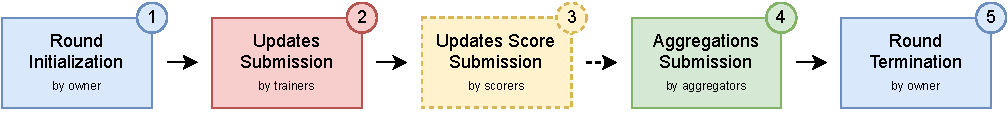
\includegraphics[width=1\textwidth]{graphics/sequence.pdf}
    \caption{BlockLearning's Execution Flow}
    \label{fig:blocklearning_steps}
\end{figure}

The framework supports a modular sequential flow represented in \autoref{fig:blocklearning_steps}. This flow is based on the current literature and the steps required to perform the Federated Learning process via the blockchain. The steps are explained below:

\begin{enumerate}
    \item The model owner initializes the round. During the round initialization, depending on the participant selection algorithm, the trainers that will participate may have been selected already, or not.
    
    \item The trainers retrieve the information such as the global weights from the last round and train the model using their local data. Then, the trainers submit their model updates.
    
    \item If a scoring algorithm is enabled, the scorers retrieve the updates and calculate the scores. Then, they submit their scores.
    
    \item The aggregators retrieve the model updates and execute the aggregation algorithm and submit the aggregation results to the blockchain.
    
    \item Finally, the model owner sends a transaction to the blockchain in order to terminate the round. At this point, the smart contract checks if the majority of the aggregators agreed on the aggregation. If so, the round is marked as terminated. Otherwise, the round fails, indicating that the aggregators did not reach an agreement, which may indicate that some of the aggregators are compromised.
\end{enumerate}

In the last step of the execution flow, the smart contract checks if the majority of the aggregators agree on the aggregation. The majority is defined by \textit{at least 50\%}. Therefore, the framework offers a 50\% threat model. However, the threat threshold can be changed, changing the threat threshold.

\subsection{Structure and Modules}\label{meth:struct_modules}

The framework is divided into three main software components: the smart contracts, the library, and the testbed. The structure of the framework, as well as its modules, is depicted on \autoref{fig:blocklearning_modules}. Each of the components plays a different part in the overall system in order to support the logical flow shown in \autoref{fig:blocklearning_steps}. In the following subsections, each of the components will be individually explained in more detail.

\begin{figure}[!ht]
    \centering
    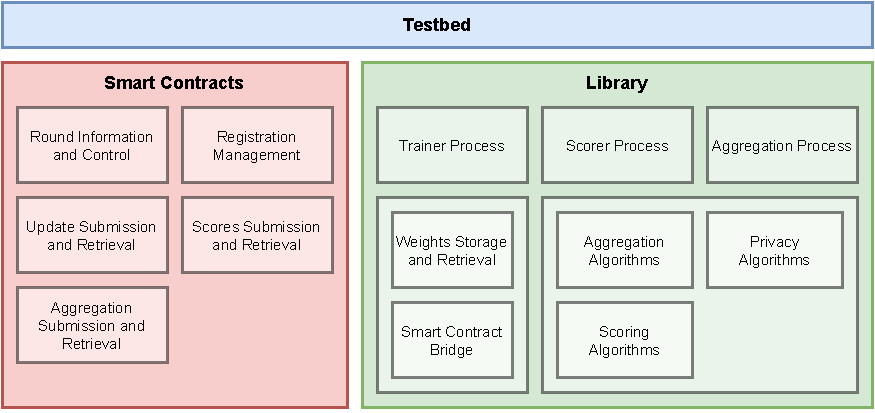
\includegraphics[width=1\textwidth]{graphics/modules.pdf}
    \caption{BlockLearning's  Structure and Modules}
    \label{fig:blocklearning_modules}
\end{figure}

\subsubsection{Smart Contracts}\label{meth:smart_contracts}

The first component of the framework is the smart contracts. The smart contracts live on the blockchain and are the main means of communication between FL clients and servers. In addition, the smart contracts hold information regarding the current status of the round, as well as the updates, scores, aggregations, among others. The smart contracts provide the following functionality:

\begin{itemize}
    \item \textit{Round Information and Control}: the smart contract must provide information on whether the round is ongoing and which phase, i.e., scoring, aggregation, or termination phase, it is in. It must allow for flexibility such that new phases can be added in the future, such as the backpropagation confirmation phase we need for our vertical model. In addition, it must allow for rounds to be started and marked as terminated. Round phase advancements are defined through pre-defined conditions that, once met, automatically move the round to the next phase. For example, after all updates are received, the smart contract should move to the next phase.
    
    \item \textit{Registration Management}: the smart contract must allow devices to register themselves as trainers, aggregators, or scorers in the system. Finally, the smart contract should provide information about which devices participate in each round.
    
    \item \textit{Update Submission and Retrieval}: the smart contract must allow trainers to submit their updates, which must include a pointer to the model weights and the amount of data points that were used to train the model. In addition, it can include the training accuracy and testing accuracy for each individual trainer. The submissions must be accessible.
    
    \item \textit{Scores Submission and Retrieval}: the smart contract must allow scorers to submit their scores. It must be possible to know which scorer scored which update and they must be accessible.
    
    \item \textit{Aggregation Submission and Retrieval}: the smart contract must allow aggregators to submit the aggregations, which contain a pointer to the weights. The aggregations must be accessible.
\end{itemize}

\subsubsection{Library}\label{meth:library}

The second component of the framework is the library. The library encodes the algorithms, utilities, and building blocks necessary to implement the scripts that run on the clients and the servers. It must include:

\begin{itemize}
    \item \textit{Aggregation, Scoring} and \textit{Privacy Algorithms}: implementation of the different algorithms. For each algorithm type, a common interface must be implemented, such that adding new algorithms is easy and simple and they are interchangeable.
    
    \item \textit{Weights Storage and Retrieval}: utilities to load and store weights on the decentralized storage provider. These must also provide an interface in order to make it easy to change the storage provider by providing a different implementation.
    
    \item \textit{Smart Contract Bridge}: a contract class that provides an interface to the smart contract that lives on the blockchain. With this class, it should be possible to call the smart contract functions as if they were local functions.
    
    \item \textit{Trainer, Scorer} and \textit{Aggregator Classes}: a class per each device category. This class must register the devices as their category upon initialization. It must also provide methods to execute the training, scoring and aggregation tasks, respectively.
\end{itemize}

\subsubsection{Testbed}\label{meth:testbed}

The third component of the framework is the testbed. The testbed provides the platform to conduct the experiments in a reproducible way, for instance by setting static seeds for randomness. The testbed must include:

\begin{itemize}
    \item \textit{Client, Server} and \textit{Owner Scripts}: scripts that will be run at the clients, the servers, and at the model owner, respectively. These scripts will use the library in order to perform the right tasks according to which algorithm is being used.
    
    \item \textit{Federated Learning Setup and Deployment}: scripts and tools to easily deploy the client and server machines in a test environment, such as containers.
    
    \item \textit{Blockchain Setup and Deployment}: scripts and tools to easily deploy the blockchain network in a test environment using the different consensus algorithms, and to deploy the contract to such network.
\end{itemize}

In addition, the testbed must also include tools to collect the required statistics and logs that can be later processed to retrieve the metrics necessary for the impact analysis.

\section{BlockLearning Framework's Implementation}

In this section, we go over the implementation details of the BlockLearning framework, following the guidelines defined in \Cref{framework:design}. The complete implementation is publicly available on GitHub\footnote{\url{https://github.com/hacdias/blocklearning}}.

\subsection{Smart Contracts}

As mentioned previously, we use the Ethereum \cite{wood2014ethereum} blockchain platform as it is the most popular and compatible with all the techniques we use for our experiments and comparison with the related work. Therefore, the smart contracts must be implemented in a programming language that supports Ethereum. We chose the Solidity \cite{solidity} programming language as it is the most well-known with the widest support.

Since our framework supports different algorithms, we need four different smart contracts. These smart contracts inherit most of their functionality from an abstract smart contract that provides the common data structures and functionality, named \texttt{Base}. Then, we implement the following classes, that derive from \texttt{Base}:

\begin{itemize}
    \item \texttt{RandomSelectionNoScoring}, which is used when we do not need a scoring algorithm. It only adds a new function to the \texttt{Base} class in order to allow the model owner to start a round with random participant selection.
    
    \item \texttt{RandomSelectionScoring}, which is used when we need a scoring algorithm. This smart contract implements the required methods to support the scoring phase, such as scoring submissions and the scoring round. In addition, it adds a function to allow the model owner to start a round with random participant selection.
    
    \item \texttt{FirstComeFirstServedNoScoring}, which is used with the first-come first-served participant selection algorithm with no scoring mechanism. It adds a function to allow the model owner to start a round with first-come first-served participant selection.
\end{itemize}

A class diagram with the public interfaces of the contracts, as well as the data types, is depicted in \autoref{fig:contracts-uml}. From the diagram, we can see that the smart contract provides round information and control, registration management, updates submission and retrieval, scores submission and retrieval, as well as aggregation submission and retrieval. One may note that the scores submission and retrieval are only implemented in \texttt{RandomSelectionScoring} as the remaining smart contracts are not used with scoring mechanisms.

\begin{figure}[!ht]
    \centering
    \centering
    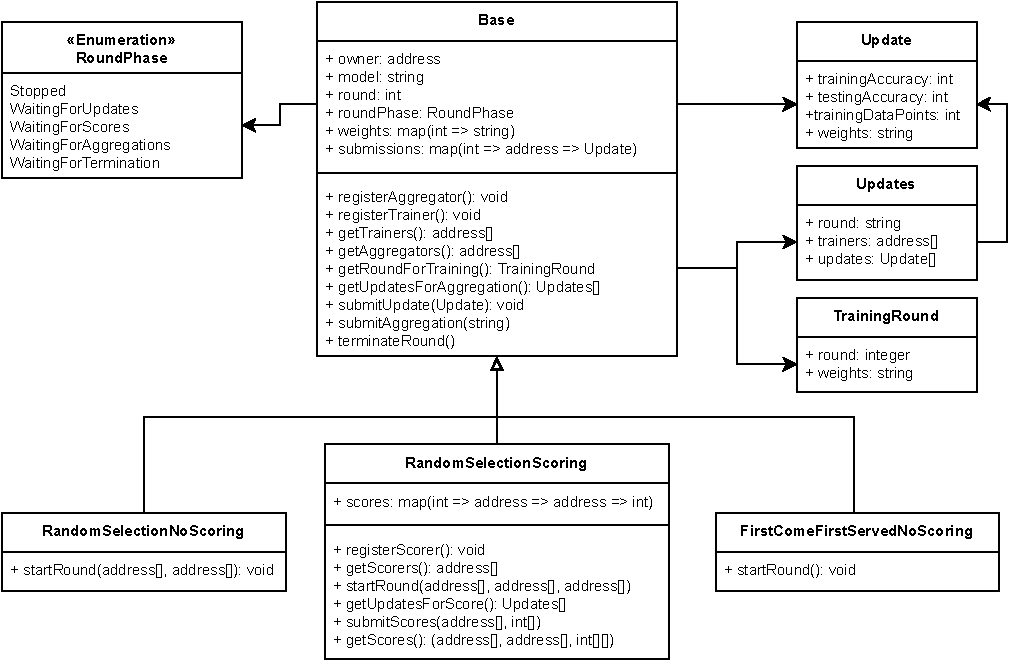
\includegraphics[width=1\textwidth]{graphics/smart-contract-uml.pdf}
    \caption{Smart Contracts Class Diagram}
    \label{fig:contracts-uml}
\end{figure}

An interesting implementation detail to note is that score and accuracy values are stored as integers. Currently, Solidity does not support floating point numbers. To preserve fidelity, the original values are multiplied by a large integer, $10^{18}$. Then, when the values are retrieved from the smart contract, they are divided by the same value in order to get the original value.

\subsection{Library}

The library is implemented in the Python \cite{10.5555/1593511} programming language. The main motivation for using Python is that many well-known Machine Learning libraries, such as TensorFlow \cite{tensorflow2015-whitepaper} and PyTorch \cite{NEURIPS2019_9015} are implemented in Python, as well as many data processing tools.

\subsubsection{Aggregation, Scoring and Privacy Algorithms}

The first component of the library is the aggregation, scoring and privacy algorithms. Each of these categories of algorithms has a specific interface to which each algorithm must conform to. By having a common interface, we can implement new algorithms, or change existing ones, easily. The interfaces are as follows:

\begin{itemize}
    \item \texttt{aggregate(trainers, updates, scorers, scores) $\rightarrow$ weights}\\
    The aggregators must provide a function \texttt{aggregate} that receives an array with the trainer addresses, an array with the updates sorted by the same order as the trainers, an array with the scorers and an array with the scores sorted by the same order as the scorers. It is important to note that the scorers and the scores are optional arguments since a scoring algorithm is not always required. The function returns an array with the aggregated weights. % BlockFlow, FedAvg, Multi-KRUM
    
    \item \texttt{score(round, trainers, updates) $\rightarrow$ trainers, scores}\\
    The scorers must provide a function \texttt{score} that receives an integer with the round number, an array with the trainer addresses, as well as an array of updates that are sorted by the same order as the trainer addresses. The function returns an array with the trainers and their submission scores. % Multi-KRUM, MarginalGain, Accuracy (BlockFlow)
    
    \item \texttt{privatize(x) $\rightarrow$ y}\\
    The privacy mechanisms must provide a function \texttt{score} that receives an array of the weights \texttt{x} and returns the privatized weights \texttt{y}. % Gaussian
\end{itemize}

Each of the aggregation and scoring algorithms is implemented based on the algorithms and details provided by the original authors. The local differential privacy is implemented using IBM's \texttt{diffprivlib} \cite{diffprivlib} library.

\subsubsection{Weights Storage and Retrieval}

The second component of the library is the utilities to store and retrieve the weights. The weights storage class also provides a common interface such that it is possible to change which storage provider we use. For our implementation, we use the InterPlanetary File System (IPFS) \cite{10.48550/arxiv.1407.3561} as our decentralized storage provider since it was used by many of the works reviewed in \Cref{chapter:related_work}.

IPFS is a distributed content addressed file system, which implies that, every file is addressed by its content. It works by attributing a hash, based on the file's content. Using this hash, also known as Content Identifier (CID), the file can be retrieved from the network and guaranteed to be immutable. Instead of storing the entire file in the blockchain, the CID can be stored. Pairing IPFS with the blockchain keeps the system decentralized and distributed, while offloading the storage to a different system.

\subsubsection{Smart Contract Bridge}\label{impl:bridge}

The third component is the smart contract bridge class. The smart contract bridge is implemented using the \texttt{Web3.py} \cite{web3py} library, which provides utilities to call the functions of the smart contracts. The contract bridge class provides 1:1 functions for each functions of the smart contract.

\subsubsection{Trainer, Scorer and Aggregator Classes}

The fourth and the final component of the library is the \texttt{Trainer}, \texttt{Scorer} and \texttt{Aggregator} classes. These classes implement the main flow of each of these procedures using the modules aforementioned described. For example, the trainer class is initialized with the contract bridge, the weights storage, the model, the data and an optional privacy mechanism. Then, it provides a method \texttt{train()} that executes the training procedure. Similarly, the scorer class provides \texttt{score()} and the aggregator class provides \texttt{aggregate()}.

\subsection{Testbed}

The testbed, that is, the platform to conduct the experiments. It was mostly implemented using the aforementioned library and Docker \cite{docker}. Docker is a platform that allows to easily deploy applications in an isolated setting through what is called a container, allowing us to simulate multiple devices in the same network. Each container runs an image, which is the name given to the piece of software than runs on the container.

In the testbed, we have two major components: the client, server and model owner scripts, the federated learning environment deployment and the blockchain deployment. These are discussed on the following subsections.

\subsubsection{Client, Server and Owner Scripts}

The client, server and model owner scripts are the processes that will run at the client, server and model owner, respectively. These are implemented using the BlockLearning library. In each of these scripts, we first load the required data, such as the data set in the clients, and initialize the required algorithms, namely the scoring, aggregation and privacy algorithms.

Then, depending on the scoring algorithm, we initialize the relevant classes at the correct machines. For example, for the BlockFlow scoring algorithm, the client initializes a \texttt{Trainer} and a \texttt{Scorer}, while the server initializes an \texttt{Aggregator}. In contrast, for Multi-KRUM, the client only initializes a \texttt{Trainer}, while the server initializes an \texttt{Aggregator} and a \texttt{Scorer}. On \autoref{alg:client_loop} you can visualize part of the main loop of the client script.

\begin{algorithm}
\caption{Client Script Main Loop}\label{alg:client_loop}
\begin{algorithmic}
\Require $s \in$ \{\O, BlockFlow, MarginalGain\}
\State $T \gets $ Initialize Trainer
\If{$s$ is not \O}
    \State $S \gets $ Initialize Scorer
\EndIf
\While{True}
    \State $P \gets$ Get Phase From Smart Contract
    \If{$P$ is Waiting For Updates}
        \State Execute Training Procedure $T.train()$
    \ElsIf{$P$ is Waiting For Scores}
        \State Execute Scoring Procedure $S.score()$
    \EndIf
\EndWhile
\end{algorithmic}
\end{algorithm}

\subsubsection{Blockchain Setup and Deployment}

The Blockchain setup and deployment is done using already existing tools and our library. As previously mentioned, we use Docker containers in order to run the experiments. Moreover, we use Docker Compose in order to deploy multiple containers at once and orchestrate the deployment process.

We use different Ethereum implementations, depending on the consensus algorithm since they are not all available within the sample implementation. Ethereum's main implementation, \texttt{go-ethereum} \cite{go-ethereum}, provides PoA and PoW. For QBFT, we use a fork called \texttt{quorum} \cite{quorum}, which is mostly identical to \texttt{go-ethereum} but supports QBFT.

Moreover, the Blockchain setup and deployment follows the following steps:

\begin{enumerate}
    \item \textit{Generate Accounts}. In first place, the Ethereum accounts for the clients and servers are generated using the provided \texttt{go-ethereum} toolkit. Each account is pre-loaded with $100$ ETH, the Ethereum currency, so that clients or servers will not run out of currency to submit their transactions.
    
    \item \textit{Build Images}. In second place, we build the Docker images that will be used to deploy the Blockchain network. This images are based on the images provided by each of the Ethereum's implementations that we use. In addition, they pre-load the account information, as well as some additional configuration to ensure that all nodes are connected when the network is bootstrapped.
    
    \item \textit{Deploy Network}. In third place, the network is deployed using Docker Compose and the configured amount of nodes.
    
    \item \textit{Deploy Contract}. Finally, the contract is deployed to the network using Truffle, which is a tool designed to help developers developing and deploying smart contracts.
\end{enumerate}

Finally, we would like to mention that originally we were planning on testing the PoS consensus algorithm. However, the only fork providing PoS support does not work in private network settings \cite{issuePos}. Therefore, it was not possible to run an experiment with PoS.

\subsubsection{Federated Learning Setup and Deployment}

Similarly to the Blockchain setup and deployment, we also use Docker Compose for the Federated Learning system. The process is identical as in the previous section, except that we only build the images and deploy the Federated Learning network.

\subsubsection{Statistics and Metrics Collection}

The different components of the library, such as the \texttt{Trainer}, \texttt{Scorer} and \texttt{Aggregator} classes, produce logs. These logs contain information related to timestamps and round number, and events that happen at certain points of the execution, such as: \textit{aggregation started}, \textit{aggregation ended}, \textit{scoring started}, \textit{scoring ended}, among others. These logs are retrieved from the containers using command-line tools implemented into a script called \texttt{toolkit.py}.

In addition, resource-related statistics, such as RAM usage, CPU usage, and network traffic, are collected directly from the Docker, through the \texttt{docker stats} command.


\chapter{Experimental Setup and Evaluation}\label{chapter:evaluation}
In this chapter, we provide information regarding the experimental setup and performance evaluation. To be more precise, this chapter explains which data set we use, how the data is partitioned, which models are used in the experiments, the software and hardware specifications of the experimental environment, as well as description of experiments we perform.

\section{Data Set}\label{eval:data_set}

The data set used for the experiments is the MNIST \cite{lecun2010mnist} data set. The MNIST data set includes 70,000 images of handwritten digits from 0 to 9, where each image is 28 by 28 pixels. Some samples are illustrated in \autoref{fig:mnist}.

\begin{figure}[!htp]
    \centering
    \centering
    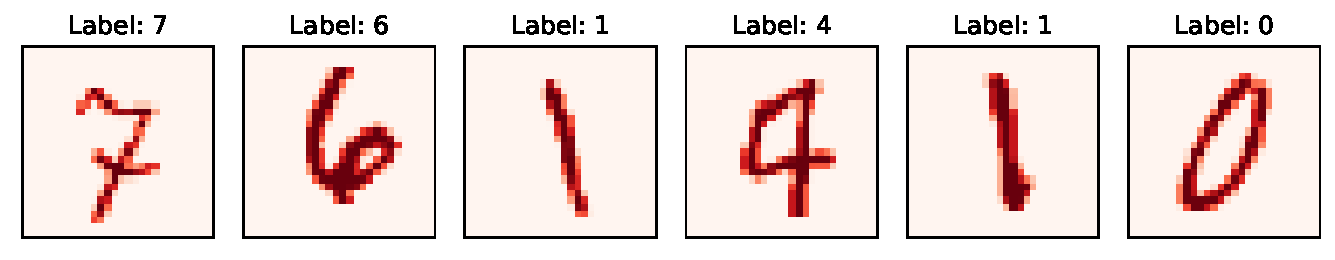
\includegraphics[width=1\textwidth]{graphics/mnist.pdf}
    \caption{MNIST Example Samples}
    \label{fig:mnist}
\end{figure}

The MINST data set is not only a well-known data set but also widely used by the majority of the reviewed works, as seen in \autoref{tab:data_distribution}. Therefore, to be able to compare our experiment results with the original works, we use the same data set.

\section{Client Sampling}\label{eval:client_sampling}

The client sampling, that is, the process of dividing the samples among the clients, depends on how data is partitioned across federated learning clients. Data may be partitioned horizontally or vertically in federated learning systems. In the following subsections, we explain how we sample the data for each of the data partitions.

\subsection{Horizontal}

In horizontally partitioned data, as explained in \Cref{background:archfl}, different clients have different samples that share the same feature space. Additionally, in a distributed system, it is expected that the clients are heterogeneous in terms of their computational characteristics and data. Therefore, it is safe to assume that the data distribution in a distributed setting is \textit{non-iid}.

To simulate a \textit{non-iid} distribution, both in terms of number of samples and number of classes at each client, we use the Dirichlet distribution \cite{tim, 10.48550/arxiv.2006.07242}. The Dirichlet distribution, $Dir(\alpha)$, is a probability distribution characterized by its parameter $\alpha$, which controls the degree of \textit{non-iid}-ness of the distribution. The higher the $\alpha$, the more identically distributed the data will be. The lower the $\alpha$, the more likely it is for each client to only hold samples of a single class.

For our experiments, we set $\alpha = 0.1$ in the Dirichlet distribution as it yields a realistic \textit{non-iid} distribution \cite{10.48550/arxiv.2006.07242}, where some clients hold many samples of a few classes, while other clients have few samples of many classes. Moreover, the clients have, on average, 2500 samples each. Some clients have more samples, some have less, simulating a \textit{non-iid} distribution.

In order to perform the horizontal client sampling, we used a publicly available tool \cite{tsingz0} that supports sampling from the MNIST data set directly using the Dirichlet distribution. We did so for 5, 10, 25 and 50 clients. \autoref{fig:horizontal_dist} illustrates the sample distribution for 10 clients. From \autoref{fig:horizontal_dist}, it is possible to see how \textit{non-iid} the distribution is, both in terms of number of data samples and class distribution. For example, client 7 has many samples from classes 2 and 4, while having none of the remaining classes. At the same time, client 10 has a few samples from classes 0, 1, 2, and 9 and many from class 7.

\begin{figure}[!ht]
    \centering
    \centering
    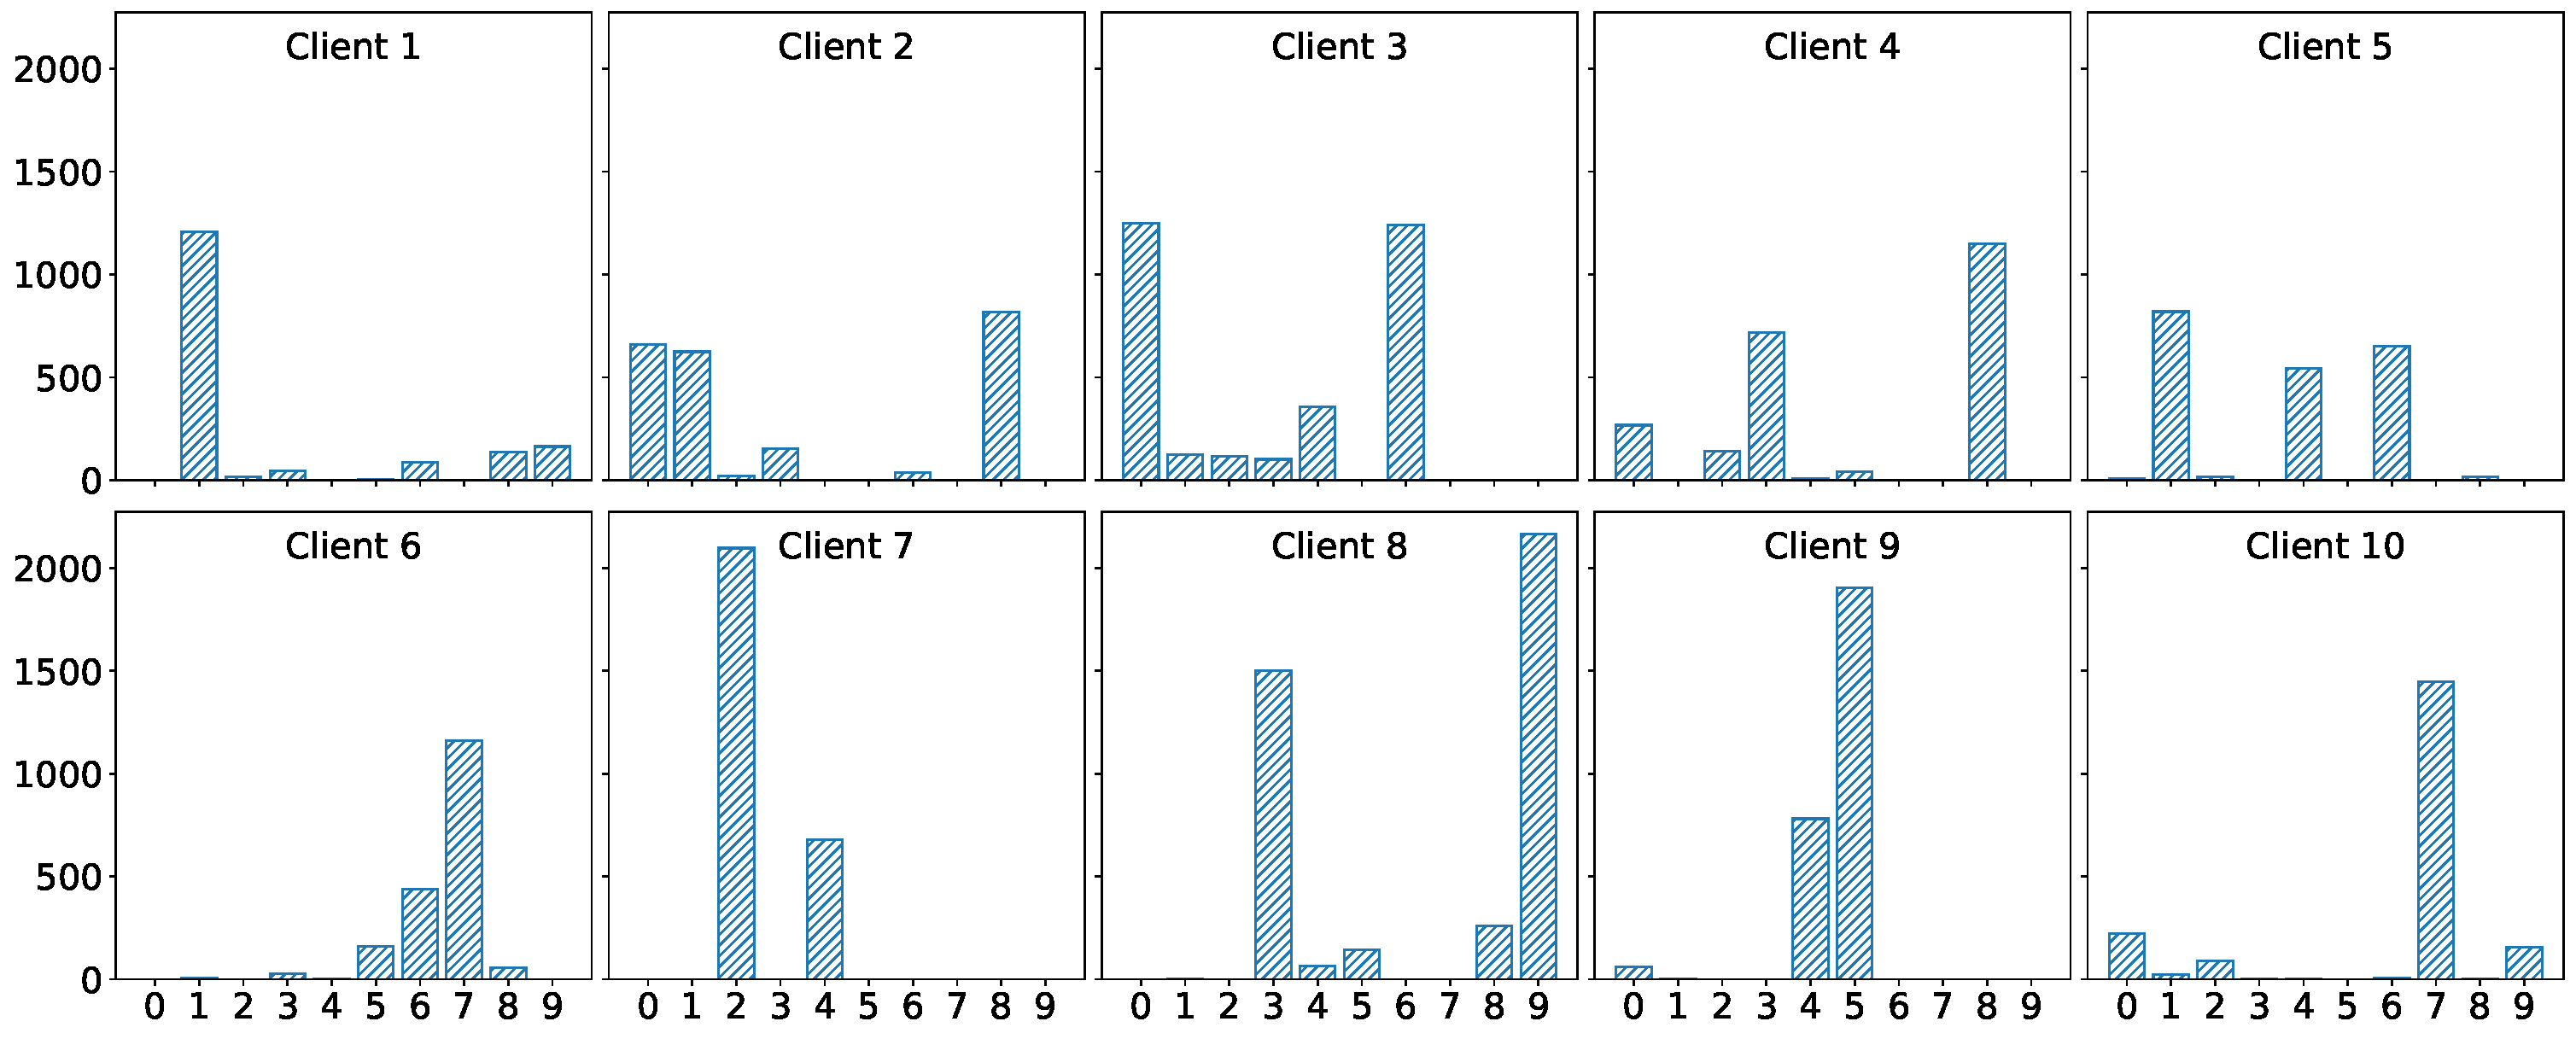
\includegraphics[width=1\textwidth]{graphics/10_dist.pdf}
    \caption{Horizontal Data Distribution For 10 Clients}
    \label{fig:horizontal_dist}
\end{figure}

\subsection{Vertical}\label{subsection:verticalpartitioning}

Vertically partitioned data is significantly different from horizontally partition data, in the sense that the clients share intersecting sample spaces, but different feature spaces. Therefore, it is not possible to simply divide the samples among the clients.

\begin{figure}[!ht]
    \centering
    \centering
    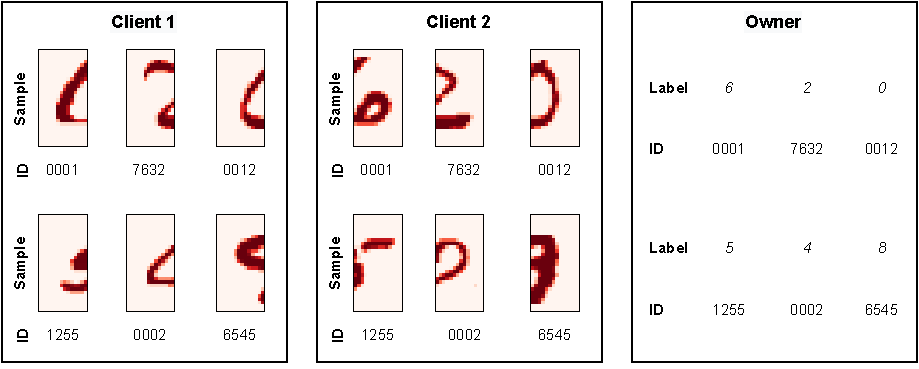
\includegraphics[width=1\textwidth]{graphics/vertical_partitioning.pdf}
    \caption{Vertical Data Distribution for 2 Clients}
    \label{fig:vertical_dist}
\end{figure}

For the vertical data partition, we use the work reported in \cite{10.48550/arxiv.2104.00489}. Firstly, we choose how many samples to assign to each client. We chose 20,000 samples in order to match the original work \cite{10.48550/arxiv.2104.00489} we will be comparing to. Then, the samples are randomly chosen from the original data set. Subsequently, each sample is assigned a unique identifier (ID) that will be used as label when giving the data samples to each client. Only the servers have access to the ground truth labels. After assigning the IDs, the feature space $F$ will be divided into $C$ parts $F_c$, where $C$ is the number of clients. Finally, the features $F_c$, with $c \in C$ will be assigned to each of the clients.

For vertical data partitioning, we divide the data set as in \cite{10.48550/arxiv.2104.00489} to use it with a Split-CNN \cite{10.1145/3297858.3304038} model, which will be introduced in the next section. To use this model, the model owner is expected to have the labels, while the clients are expected to have some features of each sample. For the MNIST data set, we can think of the features as vertical fragments of the image. To divide a 28 by 28 image sample between 2 clients, for example, we split the image into two 14 by 28 segments, as depicted in \autoref{fig:vertical_dist}.

\section{Machine Learning Models}\label{eval:ml_models}

The models used on this work are simple models found in related work. The goal of this work is not to provide the most efficient or accurate FL model. Therefore, we do not dive into the details of the models. The models used for horizontal and vertical training are succinctly explained below.

\subsection{Horizontal Model}

For the horizontal FL, we use a simple Convolutional Neural Network (CNN) \cite{cnn} with three levels of convolution intercalated with max pooling to reduce overfitting. These layers are followed by a flattening layer and two dense layers that culminate in the output. The architecture is depicted in \autoref{fig:model_cnn} and more details about its parameters can be found in \autoref{tab:cnn}. To train this model, both servers and clients have the same model. Then, the clients train the the model with their own data set. Subsequently, the clients send the weights to the servers by submitting their local model update to the blockchain via the smart contract. Finally, the servers aggregate the weights and publish the global model weights through the smart contract.

\begin{figure}[!hb]
    \centering
    \centering
    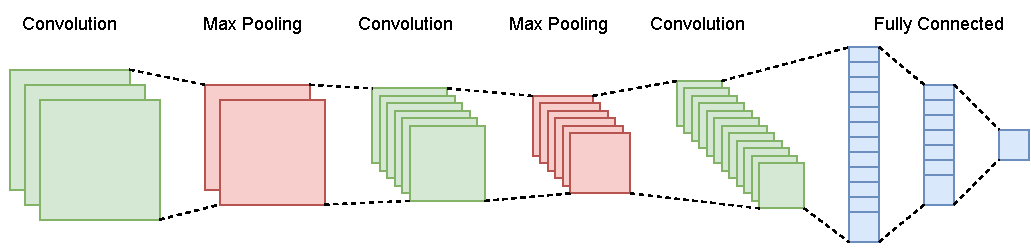
\includegraphics[width=1\textwidth]{graphics/model-cnn.pdf}
    \caption{CNN Model Architecture}
    \label{fig:model_cnn}
\end{figure}

\begin{table}[!h]
    \begin{tabular}{c|c}
        \hline \hline
        Layer Type       & Output Shape \\ \hline \hline
        Convolutional 2D & (26, 26, 32) \\ \hline
        Max Pooling 2D   & (13, 13, 32) \\ \hline
        Convolutional 2D & (11, 11, 64) \\ \hline
        Max Pooling 2D   & (5, 5, 64)   \\ \hline
        Convolutional 2D & (3, 3, 64)   \\ \hline
        Flatten          & (576)        \\ \hline
        Dense            & (64)         \\ \hline
        Dense            & (10)         \\ \hline
    \end{tabular}
    \caption{CNN Model Parameters of the Horizontal FL}
    \label{tab:cnn}
\end{table}

\subsection{Vertical Model}

For the vertical FL, we use a dual-headed, or four-headed, Split-CNN \cite{10.1145/3297858.3304038, 10.48550/arxiv.2104.00489}, depending on whether we have two or four clients. The model at the clients is the head model, while the model at the servers is the tail model. To train this model, each client gives its input data to the models and collects the output of the last layer. Then, this intermediate output is sent to the servers, which are then given to the tail model. The servers calculate the gradients, which are then backpropagated to the clients. For more details, please consult the original works where the workings of this model are given in more detail. The architecture is depicted in \autoref{fig:model_splitcnn} and more details about its parameters can be found in \autoref{tab:splitnn}.

\begin{figure}[!ht]
    \centering
    \centering
    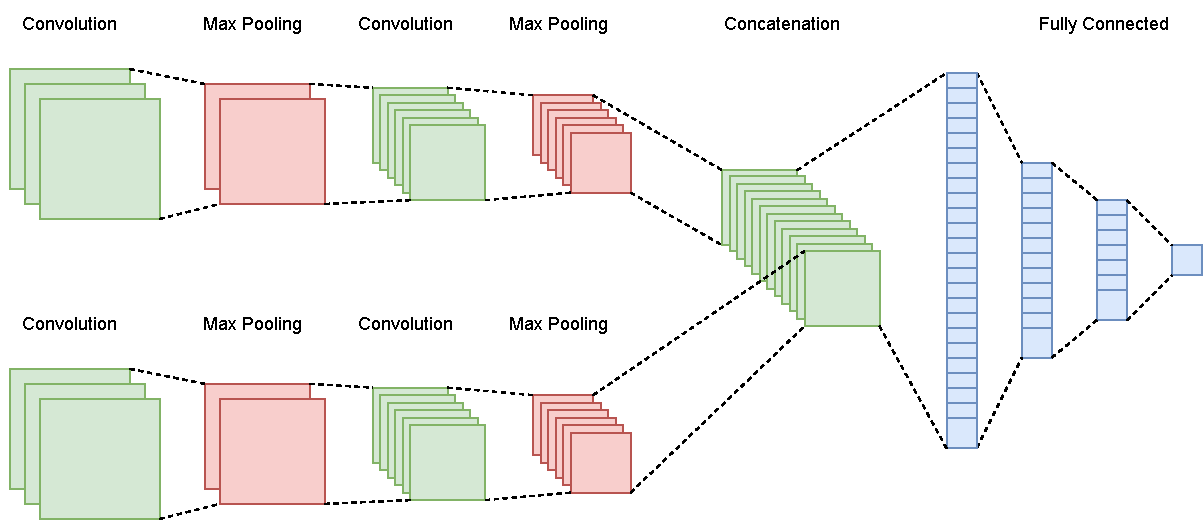
\includegraphics[width=1\textwidth]{graphics/model-splitcnn.pdf}
    \caption{Split-CNN Model Architecture}
    \label{fig:model_splitcnn}
\end{figure}

\begin{table}[!h]
    \begin{subtable}[h]{0.49\textwidth}
        \centering
        \begin{tabular}{c|c}
            \hline \hline
            Layer Type       & Output Shape \\ \hline \hline
            Convolutional 2D & (26, 12, 32) \\ \hline
            Max Pooling 2D   & (13, 6, 32) \\ \hline
            Convolutional 2D & (11, 11, 64) \\ \hline
            Max Pooling 2D   & (5, 2, 64)   \\ \hline
        \end{tabular}
        \caption{Head}
    \end{subtable}
    \hfill
    \begin{subtable}[h]{0.49\textwidth}
        \centering
        \begin{tabular}{c|c}
            \hline\hline
            Layer Type     & Output Shape \\ \hline\hline
            2 Input Layers & (5, 2, 64)   \\ \hline
            Concatenation  & (5, 2, 128)  \\ \hline
            Flatten        & (1280)       \\ \hline
            Dense          & (512)        \\ \hline
            Dense          & (256)        \\ \hline
            Dense          & (10)         \\ \hline
        \end{tabular}
        \caption{Tail}
     \end{subtable}
     \caption{Split-CNN Dual-Headed Model}
     \label{tab:splitnn}
\end{table}

\section{Hardware and Software Specifications}

The experiments were executed in a remote machine, whose hardware and software specifications can be found in \autoref{tab:temps}. Due to resource limitations, it was not possible to have a machine with GPU. Furthermore, if we consider that FL systems are being run in IoT clients, it is unlikely that such resource-constrained devices would have a GPU available. In addition, the MNIST data set and the models we used are relatively simple, which means that they can be easily trained using CPUs. Nonetheless, it is worth mentioning that the training process would likely be faster in machines with GPUs.

\begin{table}[!h]
    \begin{subtable}[h]{0.59\textwidth}
        \centering
        \begin{tabular}{l|l} \hline \hline
            Hardware & Model                                    \\ \hline \hline
            CPU      & AMD Ryzen 5 3600 6-Core 4.2 GHz          \\ \hline
            RAM      & 64 GB                                    \\ \hline
            Disk     & 500 GB NVMe                              \\ \hline
        \end{tabular}
        \caption{Hardware}
        \label{evaluation:hardware}
    \end{subtable}
    \hfill
    \begin{subtable}[h]{0.39\textwidth}
        \centering
        \begin{tabular}{l|l} \hline \hline
            Software            & Version               \\ \hline \hline
            Docker              & 20.10.15              \\ \hline
            Docker Compose      & 2.5.0                 \\ \hline
            Python              & 3.8.13               \\ \hline
            Node.js             & 16.15.0               \\ \hline
            Truffle             & 5.5.13               \\ \hline
            Ganache             & 7.1.0               \\ \hline
            Solidity            & 0.5.16               \\ \hline
        \end{tabular}
        \caption{Software}
        \label{evaluation:software}
     \end{subtable}
     \caption{Hardware and Software Specifications of Experiments}
     \label{tab:temps}
\end{table}

\section{Performance Evaluation Metrics}\label{eval:metrics}

We select the following metrics for our performance evaluation: execution time, transaction costs, transaction latency, model accuracy and convergence, communication costs, and computation costs.

\subsection{Execution Time}

To compare execution time, we define two metrics: the \textit{End-to-end (E2E) Execution Time} and the \textit{Mean Round Execution Time}. The former is defined by the time it takes for an experiment to be executed from start to the end. The latter is defined by the mean time it takes to complete an experiment round, which can be calculated by dividing the E2E Execution Time by the number of rounds of the experiment.

\subsection{Transaction Costs and Transaction Latency}

To compare the blockchain costs, namely the impact of waiting for transactions, we define two metrics: the \textit{Transaction Latency} and the \textit{Transaction Cost}. The former is defined as the mean time it takes between submitting a transaction and it being accepted by the network. The latter is defined by the mean computation effort to execute a transaction, which, in the case of Ethereum, is measured in \textit{Gas}.

Both the transaction latency and transaction cost values are retrieved directly from the Blockchain. Ethereum provides information on how much time transactions take to be accepted, as well as how much each transaction costs. Then, we only calculate the mean.

\subsection{Model Accuracy}

To compare the model accuracy, we use a global \textit{Accuracy} metric for the FL model, where the model owner, that is, the one that initiates the process, has some data set with which it can test the model. The logs produced by the model owner contain the accuracy and are used to extract the accuracy of each round.

\subsection{Communication and Computation Costs}

To compare the communication costs, we define the \textit{Network Traffic Per Round} metric, which is defined by how much network traffic flows to and from each process. It is collected for the client, server, and blockchain processes individually. By knowing the network traffic required for each process, we can draw conclusions regarding how the network traffic impacts different types of devices. For example, if there is a high volume of traffic per round at the client process, and the clients are resource-constrained IoT devices with low network bandwidth, then it is expected that each round takes longer since less traffic can go through the device at a single point in time.

To compare the computation costs, we collect the \textit{RAM Usage} and \textit{CPU Usage}.

The communication and computation costs metrics are collected at the client, server, and blockchain processes in order to be able to differentiate the effects of the different algorithms on the different parts of the system. However, it is important to note that, in practical settings, the server process and the blockchain process run on the same device.

To collect these metrics, we use \texttt{docker stats}, which is a command provided by Docker, the platform used for BlockLearning's Testbed. The statistics command provides a live stream of the container's resource consumption, namely the CPU percentage, the RAM memory usage, and the network traffic in and out.

\section{Experiment Groups}\label{meth:experiments}

The conducted experiments can be divided into three groups, of which two analyze how using different types of algorithms impact the system's performance in terms of model accuracy, convergence, communication, and computation costs. These two groups relate to impact analysis of:

\begin{enumerate}
    \item \textit{Consensus Algorithms}: PoA, PoW, and QBFT. Consensus algorithms are a component of the blockchain and they are expected to impact Horizontal Federated Learning and Vertical Federated Learning equally.
    
    \item \textit{Horizontal Federated Learning}
    
    \begin{enumerate}
        \item \textit{Participant Selection Mechanisms}: random selection versus first-come first-served.
        
        \item \textit{Scoring Algorithms}: BlockFlow, Multi-KRUM, Marginal Gain, as well as without any scoring algorithm. For each scoring algoritm, we also analyse the impact of:
        
        \begin{enumerate}
            \item \textit{Number of Clients}: 5, 10, 25, 50, selected based on the current literature and available resources we have at our disposal to execute the experiments.
            
            \item \textit{Privacy Degree}: 1 and 5, as well as without any privacy mechanism.
        \end{enumerate}
    \end{enumerate}
\end{enumerate}

In the third and last experiment group, we investigate if it is possible to implement and run a Blockchain-based Federated Learning with vertically partitioned data. To do so, we analyze how to extend the BlockLearning framework in order to support the Split-CNN model. Then, we implement the required extensions to the framework. Finally, we execute the experiments and compare the results with the original work where the Split-CNN model was used with the MNIST dataset in order to validate our experiment.

As explained in \Cref{background:archfl}, Vertical Federated Learning systems have an additional step, in which the Private Set Intersection (PSI) of the client's data sets is calculated. In this work, we assume that the PSI is calculated beforehand and that it is already known to all devices. The PSI calculation can be done in different ways and it is its own area of research of Computer Science. The related works we analyzed either did not provide information on how this was calculated, or also assumed that is has been calculated beforehand. In future works, it would be interesting to integrate a PSI mechanism into the framework.

All experiments were performed for 50 rounds so that we can compare the model accuracy results to other papers. This way, we can validate if our experiments are within the expected values. Secondly, all experiments were performed with 10 servers that run both the server process and the blockchain process. Thirdly, all experiments, except for those where the number of clients are compared, are run with 25 clients.


\chapter{Impact Analysis of Consensus Algorithms}\label{chapter:analysis:consensus_algorithms}
In this chapter, we analyze the first experiment group, that is, the impact of using different consensus algorithms on the Blockchain-based Federated Learning system. The consensus algorithms are part of the blockchain itself. Therefore, they do not impact horizontal and vertical FLs differently. In this set of experiments, all properties of the system are fixed, except for the consensus algorithm, which varies between PoA, PoW and QBFT.

\section{Execution Time, Transaction Cost, and Transaction Latency}

The first performance evaluation metrics we look into are the mean time it takes for a round to complete, the mean transaction latency, and the mean transaction cost. These values are presented in \autoref{tab:metrics_consensus_algorithms}.

\begin{table}[!ht]
\centering
\begin{tabular}{c|c|c|c} \hline \hline
Metric                              & PoA    & PoW    & QBFT   \\ \hline \hline
E2E Time (m)            & 18.93  & 30.62  & 18.97  \\ \hline
Mean Round Time (s)             & 22.70  & 36.72  & 22.74  \\ \hline
% Median Time Per Round (s)           & 21.90  & 35.28  & 21.99  \\ \hline \hline
Mean Transaction Latency (s)    & 1.549  & 1.821  & 1.558  \\ \hline
% Median Latency Per Transaction (s)  & 1.549  & 1.554  & 1.555  \\ \hline \hline
Mean Transaction Cost (Gas)     & 183124 & 227052 & 182880 \\ \hline
% Median Cost Per Transaction (Gas)   & 185198 & 229866 & 185068 \\ \hline \hline
\end{tabular}
\caption{Execution Time, Transaction Cost, and Latency of Consensus Algorithms}
\label{tab:metrics_consensus_algorithms}
\end{table}

Regarding time, we can observe that different consensus algorithms can lead to very different execution times. On the one hand, PoA and QBFT are the fastest consensus algorithms, providing the lowest execution times. Additionally, the difference between both is minimal, i.e., only $0.04$ seconds per round. On the other hand, PoW takes the longest, being $1.6$ times slower than both PoA and QBFT.

Transaction latency and costs follow a similar trend as the execution times. Both PoA and QBFT have similar transaction latency and cost, differing with a small amount, while PoW has a higher transaction latency and cost. PoW costs are $1.2$ times higher than PoA and QBFT.

As explained in \autoref{background:consensus_algorithms}, PoW works by solving increasingly complex mathematical equations that consumes high amounts of resources. This intense process can lead to slower response rates, which translates to higher transaction latency and costs. This, in turn, increases the time it takes for each round to complete.

\section{Model Accuracy and Convergence}

The model accuracy, as well as the convergence, as it can be seen in \autoref{fig:accuracy_consensus_algorithms}, does not change significantly per consensus algorithms. Consensus algorithms determine the order, at which the transactions are processed and ensure consistency between the multiple blockchain nodes. This only affects the blockchain internal processes, and not the ML process. Therefore, it was not expected that the consensus algorithms would have an impact on the model accuracy.

\begin{figure}[!ht]
    \centering
    \centering
    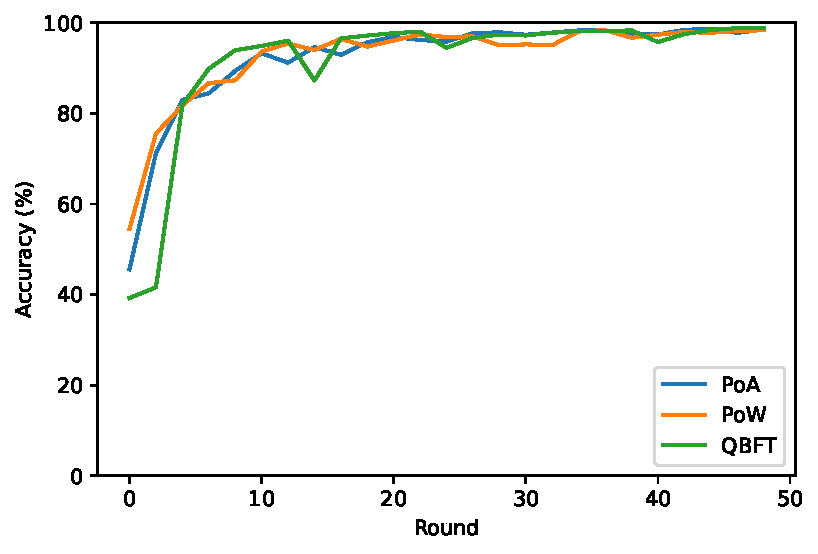
\includegraphics[width=0.7\textwidth]{graphics/consensus/accuracy.pdf}
    \caption{Accuracy Per Consensus Algorithm}
    \label{fig:accuracy_consensus_algorithms}
\end{figure}

\section{Communication Costs}

For the communication costs, we analyze the inbound and outbound network traffic per round at the client, server, and blockchain processes. These values can be observed in \autoref{fig:net_consensus_algorithms}.

On one hand, the inbound and outbound traffic for the clients and server have negligible differences when using different consensus algorithms. As mentioned in the previous section, the consensus algorithms have no expected impact on the ML process. Since the clients and servers only concern the ML process, it was expected that the clients and servers would not be affected. The small differences, in the order of $< 2$ MB, we can observe on the servers are likely related to fluctuations in the random participant selection algorithm. If more participants are being selected, more data needs to be transmitted, and vice-versa. In this case, 17.9, 18.3, and 17.7 clients participated in each round, on average, for PoA, PoW and QBFT, respectively.

On the other hand, the traffic at the blockchain process varies considerably depending on the consensus algorithm used. On average, PoW requires more bandwidth per round than PoA, but the difference is minimal. However, QBFT requires $2$ times more network traffic than PoW and $4$ times more traffic than PoA. QBFT is a three-phase consensus algorithm, which requires a higher number of network messages to be transmitted before reaching a consensus. In addition, the size of the messages also differs. When combining both of these aspects, we can conclude that the expected network traffic per round using the QBFT algorithm would be higher, as verified.

\begin{figure}[!ht]
    \centering
    \centering
    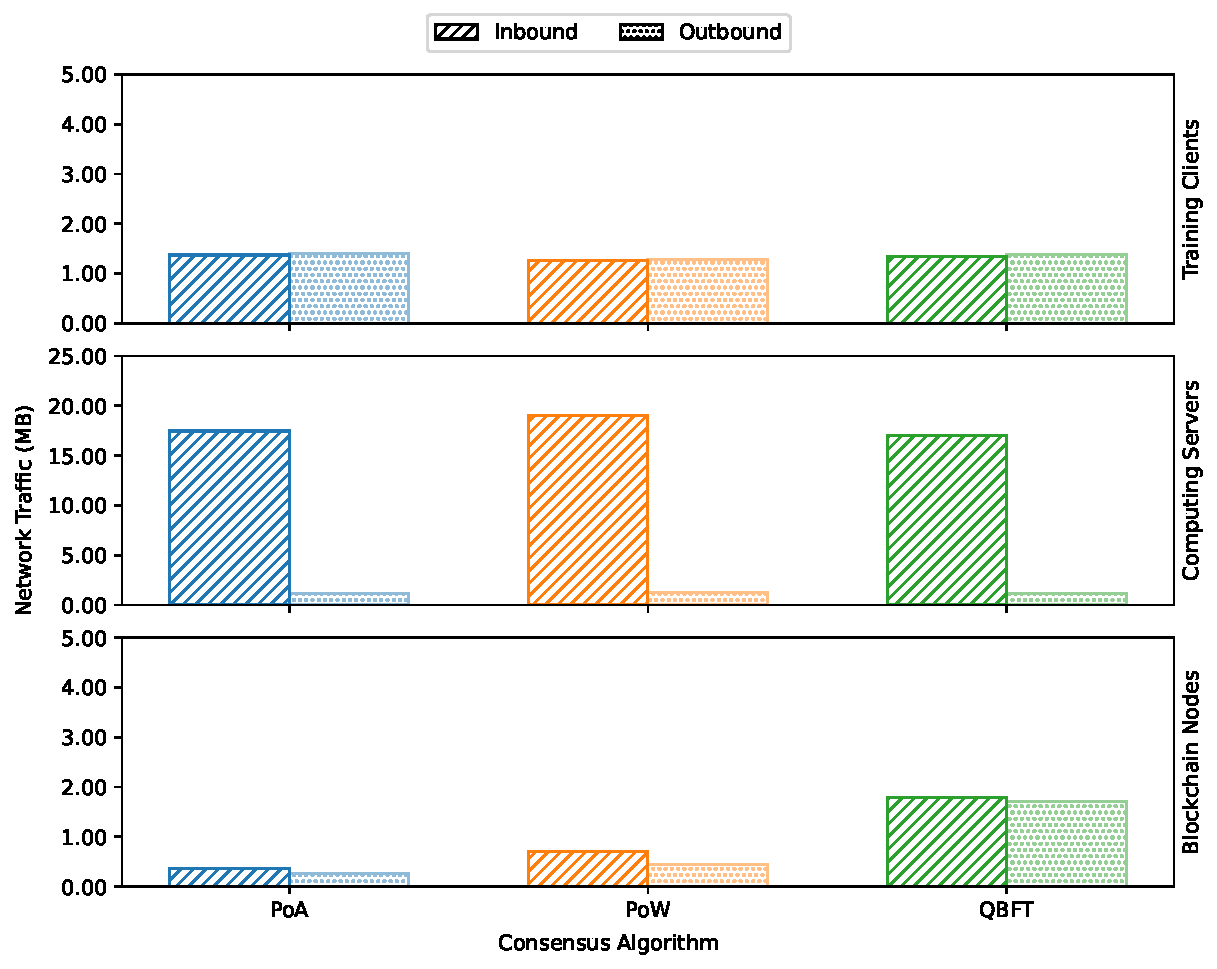
\includegraphics[width=0.8\textwidth]{graphics/consensus/net.pdf}
    \caption{Network Traffic Per Round Per Consensus Algorithm}
    \label{fig:net_consensus_algorithms}
\end{figure}

\section{Computation Costs}

Regarding computation costs, we look at both RAM and CPU usage on the client, server, and blockchain processes. \autoref{fig:ram_consensus_algorithms} and \autoref{fig:cpu_consensus_algorithms} show the mean RAM usage and mean CPU usage, respectively, per consensus algorithm during the execution of the experiments. As mentioned previously, the execution times for PoA and QBFT are lower than for PoW, which can be seen in the figures by not showing more data past minute 19. Additionally, as explained before, the consensus algorithms are not expected to have a direct impact on the clients or the servers.

\begin{figure}[!hpt]
    \centering
    \centering
    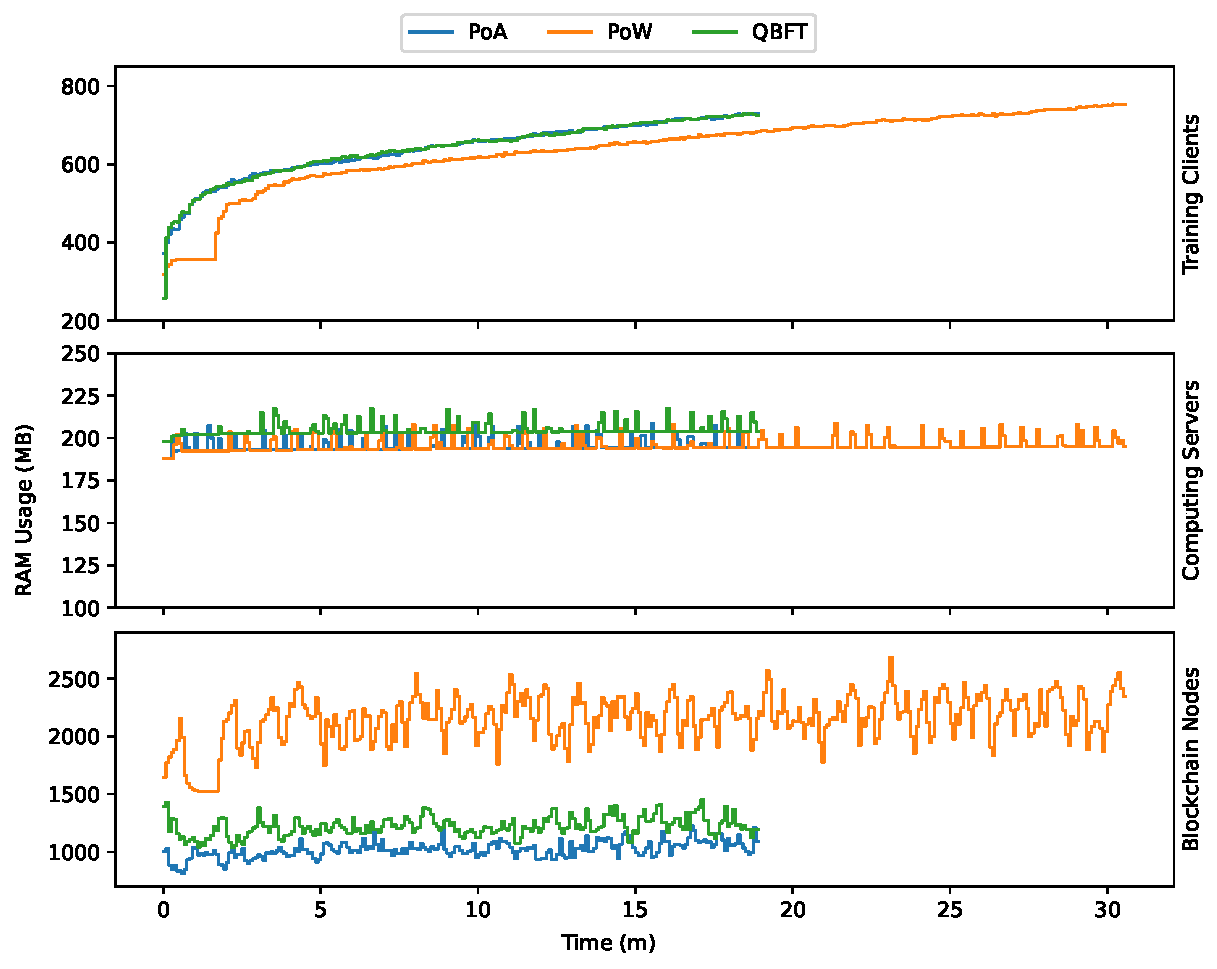
\includegraphics[width=0.8\textwidth]{graphics/consensus/ram.pdf}
    \caption{RAM Usage Per Consensus Algorithm}
    \label{fig:ram_consensus_algorithms}
\end{figure}

\begin{figure}[!hpb]
    \centering
    \centering
    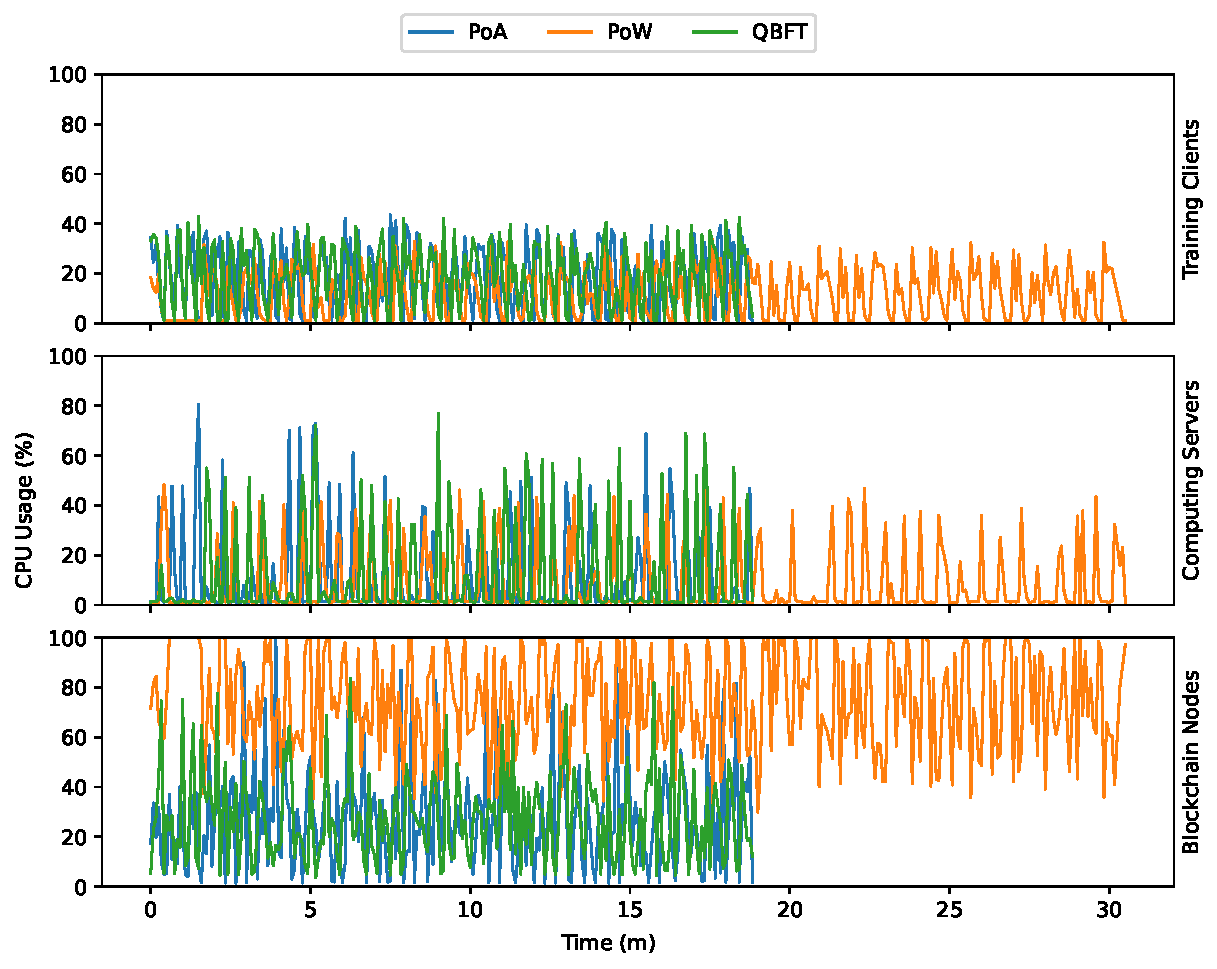
\includegraphics[width=0.8\textwidth]{graphics/consensus/cpu.pdf}
    \caption{CPU Usage Per Consensus Algorithm}
    \label{fig:cpu_consensus_algorithms}
\end{figure}

Regarding the clients, the RAM usage and CPU usage do not differ significantly regardless of which consensus algorithm is used. From the RAM usage, we observe that the clients reach the same peak. However, the rate at which that peak is reached is different. For PoW, since there are higher transaction latencies, it takes longer to reach the next round, leading to a slower growing RAM usage during the model training phase. On the other hand, from the CPU usage, we observe that there are more idle moments, that is, moments at which the CPU usage is lower. This can also be explained by the higher transaction latencies, during which the clients cannot do anything other than wait for the transaction to be approved.

Regarding the servers, the same reasoning as for the clients can be applied. While the RAM usage is consistent across different consensus algorithms, we notice that when using QBFT, the RAM usage at the servers is slightly higher. However, this is a likely negligible difference, as the difference is minimal ($< 10$ MB) considering the total RAM Usage ($\approx 200$ MB). The CPU usage is similar to what we observed for the clients, with a higher amount of idle moments.

Regarding the blockchain process, we observe a larger difference, both in terms of RAM and CPU usages. For both, PoW consumes a much higher level of resources. On average, PoW consumes $2$ times more then RAM and has a $2$ times higher CPU usage. This can also be explained by the way PoW works by solving complex mathematical equations, which require intense computation resources.

\section{Conclusions and Improvements}

In conclusion, we can observe that different consensus algorithms have no direct impact on the model accuracy and computation and communication costs at the clients and servers. However, they have an impact on the time and computation and communication costs at the blockchain process. PoA and QBFT are much faster than PoW. In addition, they require less computation power, both in RAM and CPU. However, QBFT consumes incurs more communication costs than both PoA and PoW. Therefore, there is a clear correlation between the computation costs and the time it takes. The higher the communication costs, the higher the transaction latencies, which translates to slower round times.

Assuming that the blockchain network is only being used for FL, PoA is the most cost-effective of the consensus algorithms we analyzed.

It is also worth pointing out that, as discussed in \Cref{chapter:related_work}, PoA is criticized for not being as decentralized as the other algorithms due to the way the validator nodes are chosen. If a higher degree of decentralization is required, as in a public network for example, PoW and QBFT may be better options. There is therefore a trade-off between the degree of decentralization and the communication and computation consumption.

For future work, it would be interesting to study if the Ethereum blockchain could be adapted to easily incorporate the custom consensus algorithms that were seen in \Cref{related_work:consensus_algorithms}. These algorithms work by producing proofs directly from the Machine Learning process. This can lead to better usage of resources if the blockchain network is solely used for a FL system.

\chapter{Impact Analysis of Participant Selection and Scoring Algorithms in Horizontal Blockchain-based Federated Learning}\label{chapter:horizontal}
In this chapter, we analyze the impact of using different participant selection and scoring algorithms on a Blockchain-based Federated Learning (BFS) system with horizontal data partition. In addition, for each scoring algorithm, we analyze how they behave and how the system is impacted by different number of clients, as well as privacy degrees. Due to the high number of plots, the communication and computation costs plots are placed at the end of the chapter.

\section{Participant Selection Algorithms}

In this set of experiments, all properties of the system are fixed, except for the participant selection algorithm, which can be either random selection or first-come first-served.

Both algorithms choose the number of clients in the same way, via a uniform random distribution. However, the clients themselves are chosen differently. Consequently, it is possible that the distribution of chosen clients is slightly different, which may affect the system performance. \autoref{fig:participations_client} illustrates client participation (represented by the bars), as well as the average number of participation per client (represented by the lines). It is clear from the plot that the distributions are different.

\begin{figure}[!ht]
    \centering
    \centering
    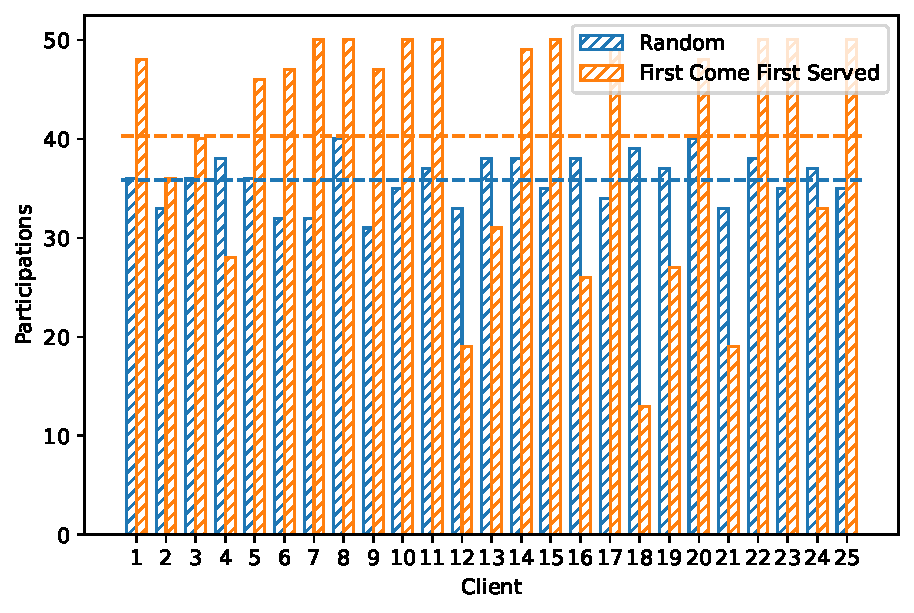
\includegraphics[width=0.7\textwidth]{graphics/selection/clients.pdf}
    \caption{Participation of Each Client Per Selection Algorithm}
    \label{fig:participations_client}
\end{figure}

On one hand, random selection presents a more uniform distribution, where each client was selected a similar number of times. On the other hand, first-come first-served presents a more skewed distribution, where some clients, such as client 1, participate many times and others, such as client 12, participate very few times. To support this observation, we calculated the standard deviation. For the random selection, the standard deviation is approximately 2.49, while for the first-come first-served it is 11.84.

From this observations, we can conclude that, by letting clients take initiative to join a round, similarly to what happens in first-come first-served, it is possible that some will end up participating more than others. By participating more often, the clients will have more influence on the global model, which can lead to skewed results.

\subsection{Execution Time, Transaction Cost, and Transaction Latency}

Regarding execution time, it can be seen from  \autoref{tab:metrics_selection} that both algorithms only differ in approximately $1.2$ minutes, which translates to a difference of $1.1$ seconds per round. In addition, the random participation was slightly faster than the first-come first-served. This negligible difference is likely caused by the fact that, in random selection, less clients participated on average per round, as shown in \autoref{fig:participations_client}. With slightly less clients, we expect that a round takes slightly less time.

\begin{table}[!ht]
\begin{tabular}{c|c|c} \hline \hline
                              & First Come First Served & Random \\ \hline \hline
E2E Time (m)                   & 19.70                   & 18.93  \\ \hline
Mean Round Time (s)            & 23.62                   & 22.70  \\ \hline
% Median Round Time (s)          & 22.06                   & 21.90  \\ \hline
Mean Transaction Latency (s)   & 1.560                   & 1.549  \\ \hline
% Median Transaction Latency (s) & 1.561                   & 1.549  \\ \hline
Mean Transaction Cost (Gas)    & 189179                  & 183124 \\ \hline
% Median Transaction Cost (Gas)  & 223471                  & 185198 \\ \hline
\end{tabular}
\caption{Execution Time, Transaction Cost, and Transaction Latency Per Participant Selection Algorithm}
\label{tab:metrics_selection}
\end{table}

\subsection{Model Accuracy and Convergence}

As it can be seen from \autoref{fig:accuracy_selection}, even though both algorithms reached identical model accuracy values at the last round, the random selection was more stable during the initial 20 rounds. This can be explained by the fact that the distribution of clients participating in each round with the random selection was closer to a uniform selection. Since the data is \textit{non-iid}, by having the same clients participate repeatedly, the model can become skewed towards their data. However, after 20 rounds, the majority of the clients had the opportunity to participate in the model, which explains why it became more and more stable.

\begin{figure}[!ht]
    \centering
    \centering
    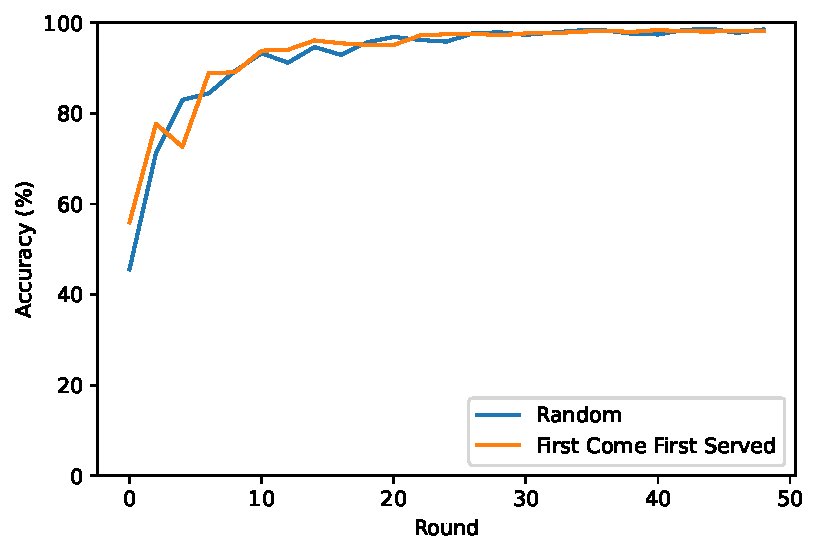
\includegraphics[width=0.7\textwidth]{graphics/selection/accuracy.pdf}
    \caption{Model Accuracy Per Participant Selection Algorithm}
    \label{fig:accuracy_selection}
\end{figure}

\subsection{Communication Costs}

\autoref{fig:net_selection} illustrates the network traffic per round for client, servers, and the blockchain processes. This algorithms solely influences which and how many clients are selected per round. Therefore, the individual communication traffic of each process is not expected to change significantly as long as the number of participants per round does not change significantly. In these experiments, we observe form \autoref{fig:participations_client} that the difference of clients participating per round is smaller than $5$. This small difference explains why the inbound traffic at the server process is slightly higher, since the server has to download weights from a higher number of clients in order to perform the aggregation.

\begin{figure}[!hpt]
    \centering
    \centering
    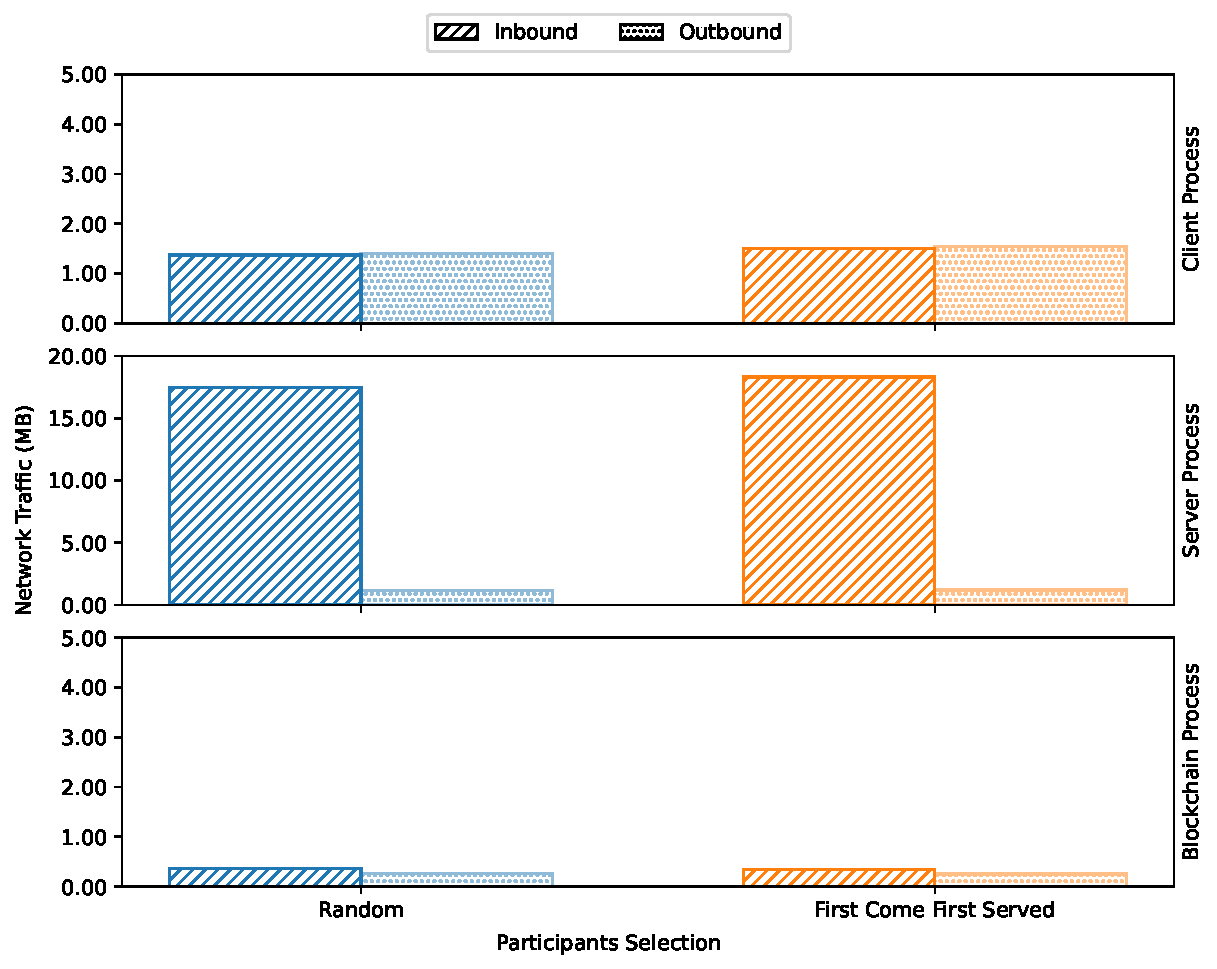
\includegraphics[width=0.8\textwidth]{graphics/selection/net.pdf}
    \caption{Network Traffic Per Round Per Participant Selection Algorithm}
    \label{fig:net_selection}
\end{figure}

\subsection{Computation Costs}

\autoref{fig:ram_selection} and \autoref{fig:cpu_selection} show the RAM usage and CPU usage per each process, respectively. Similarly to what was observed regarding the communication costs, the RAM usage at the server is slightly higher, which is explained by the additional weights to perform the aggregation. One may note that this difference happens due to the randomness of the process. In other runs, it is possible that the number of selected devices would be lower and therefore the difference would be smaller.

\begin{figure}[!hpb]
    \centering
    \centering
    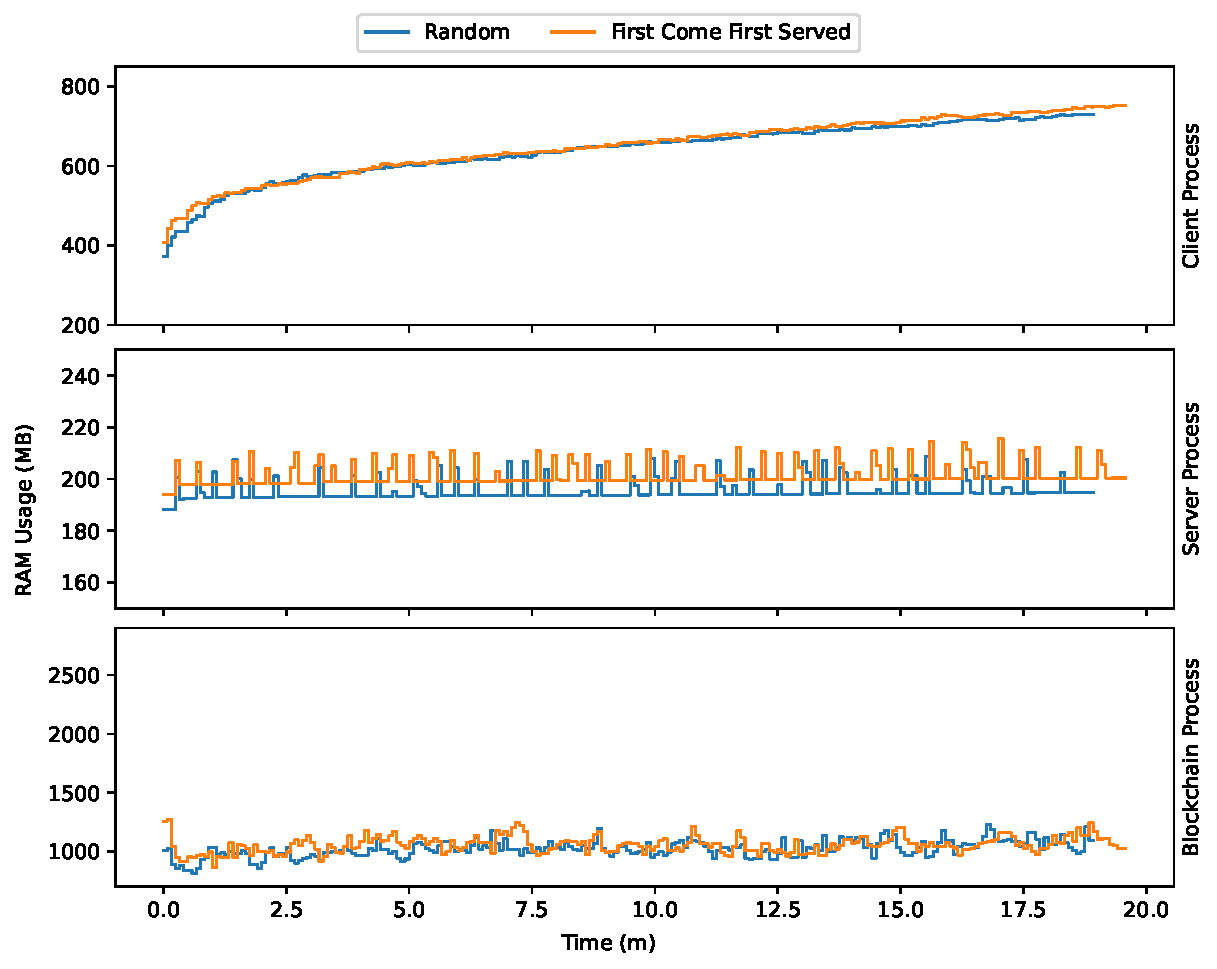
\includegraphics[width=0.8\textwidth]{graphics/selection/ram.pdf}
    \caption{RAM Usage Per Participant Selection Algorithm}
    \label{fig:ram_selection}
\end{figure}

\begin{figure}[!h]
    \centering
    \centering
    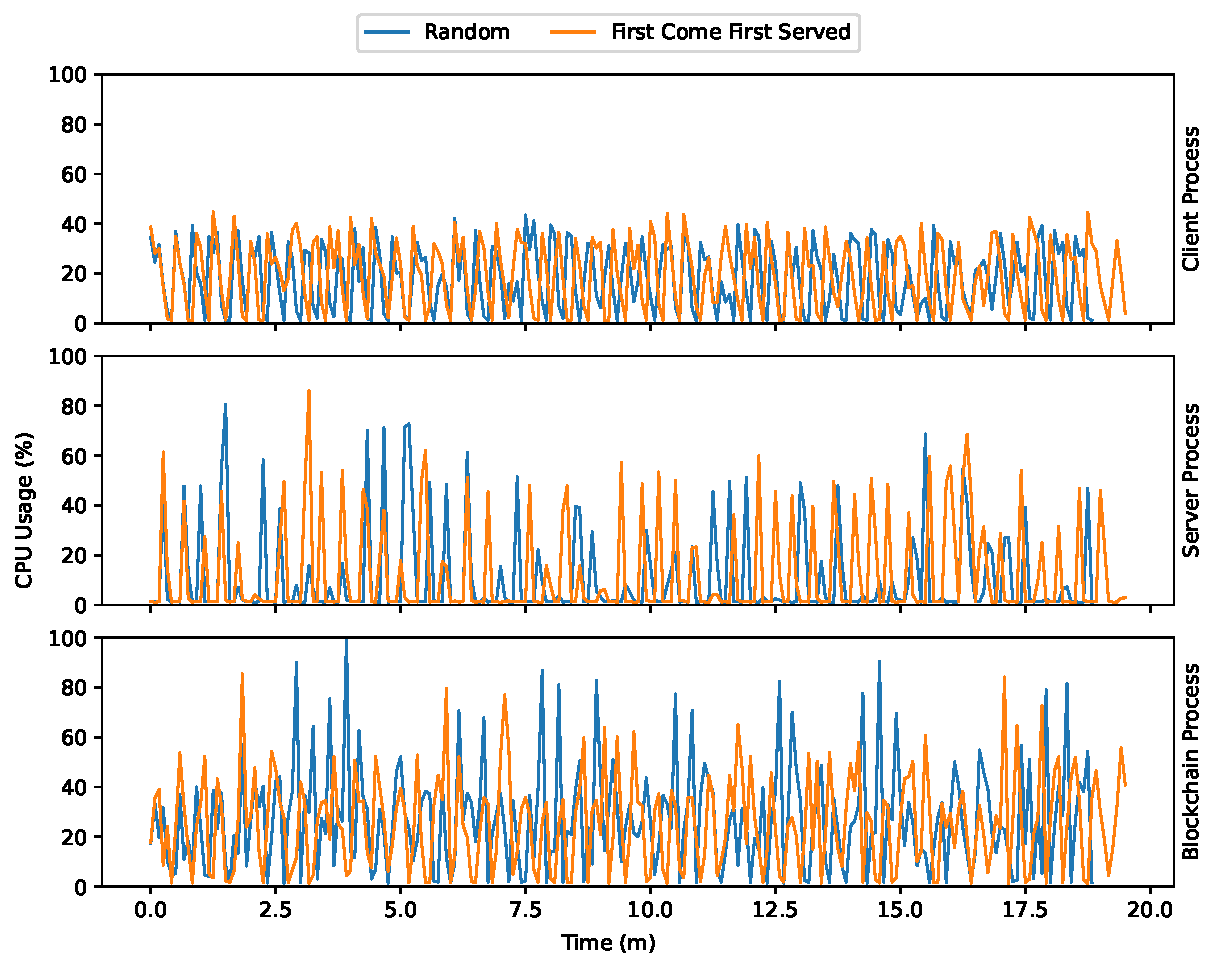
\includegraphics[width=0.8\textwidth]{graphics/selection/cpu.pdf}
    \caption{CPU Usage Per Participant Selection Algorithm}
    \label{fig:cpu_selection}
\end{figure}

\subsection{Conclusions}

From this set of experiments, we conclude that random selection performs better in terms of fairness of selection, that is, every client is given an equal chance of participating during the training process. In systems with \textit{non-iid} data, it is important to give all clients a chance to participate such that the model is trained with the most diverse data in order to produce the best results. Use of the random selection can ensure that the most amount of data is seen from most clients.

\section{Scoring Algorithms}

In this set of experiments, all properties of the system are fixed, except for the scoring algorithm, which varies between BlockFlow, Marginal Gain, Multi-KRUM, or no scoring algorithm. Then, we analyze the impact of using different numbers of clients, as well as different privacy degrees.

\subsection{Overall Comparison}\label{horizontal:scoring_overall}

We first compare the impact of the different scoring algorithms on the overall system without varying the number of clients or the privacy degree. This will let us draw some initial conclusions about the different scoring algorithms that may help explain differences observed in the remaining experiments.

\subsubsection{Execution Time, Transaction Cost, and Transaction Latency}

As it can be seen from \autoref{tab:metrics_scoring}, every scoring algorithm has different execution time and transaction cost. Firstly, one may notice that not using a scoring algorithm provides the fastest execution time as well as the lowest transaction cost. Both of these observations are explained by the fact that scoring algorithms require more transactions to submit the scores. Overall, the fastest scoring algorithm is Multi-KRUM, taking around $31$ seconds per round, while both BlockFlow and Marginal Gain are the slowest, taking both around $49$ seconds per round.

\begin{table}[!ht]
\centering
\begin{tabular}{c|c|c|c|c} \hline \hline
                               & None   & BlockFlow & Marginal Gain & Multi-KRUM \\ \hline \hline
E2E Time (m)                   & 18.93  & 40.95     & 41.38         & 26.25      \\ \hline
Mean Round Time (s)            & 22.70  & 49.11     & 49.64         & 31.48      \\ \hline
% Median Round Time (s)          & 21.90  & 49.49     & 43.97         & 31.26      \\ \hline
Mean Transaction Latency (s)   & 1.549  & 1.564     & 1.577         & 1.573      \\ \hline
% Median Transaction Latency (s) & 1.549  & 1.558     & 1.564         & 1.551      \\ \hline
Mean Transaction Cost (Gas)    & 183124 & 339645    & 257686        & 280733     \\ \hline
% Median Transaction Cost (Gas)  & 185198 & 189092    & 188994        & 187152     \\ \hline
\end{tabular}
\caption{Execution Time, Transaction Cost, and Transaction Latency Per Scoring Algorithm}
\label{tab:metrics_scoring}
\end{table}

Secondly, we observe that BlockFlow and Marginal Gain not only take the longest, but also have similar execution times. As explained in \Cref{background:scoring}, BlockFlow and Marginal Gain scores are computed by the clients, whereas Multi-KRUM scores are computed by the servers. Since the number of clients is higher than the servers, which are fixed, there are more devices performing scoring computations with BlockFlow and Marginal Gain. With more devices submitting scores, there are more transactions being submitted to the blockchain, leading to higher execution times. Therefore, it is expected that algorithms that run on the clients, such as BlockFlow and Marginal Gain, take longer than algorithms that run on the servers, such as Multi-KRUM.

Thirdly, we observe that the transaction latency is not influenced by the scoring algorithms. As it can be seen form \Cref{chapter:analysis:consensus_algorithms}, the transaction latency is mostly affected by the blockchain consensus algorithms, which, in these experiments, is fixed. In contrary, the transaction costs vary per scoring algorithm. Scoring algorithms that have more devices involved, such as scoring algorihtms executed by the servers, namely BlockFlow and Marginal Gain, have higher transaction costs. Since transaction costs work on a "supply and demand" basis, it is expected that the more transactions are required, the higher the cost will be.

\subsubsection{Model Accuracy and Convergence}

\begin{figure}[!ht]
    \centering
    \centering
    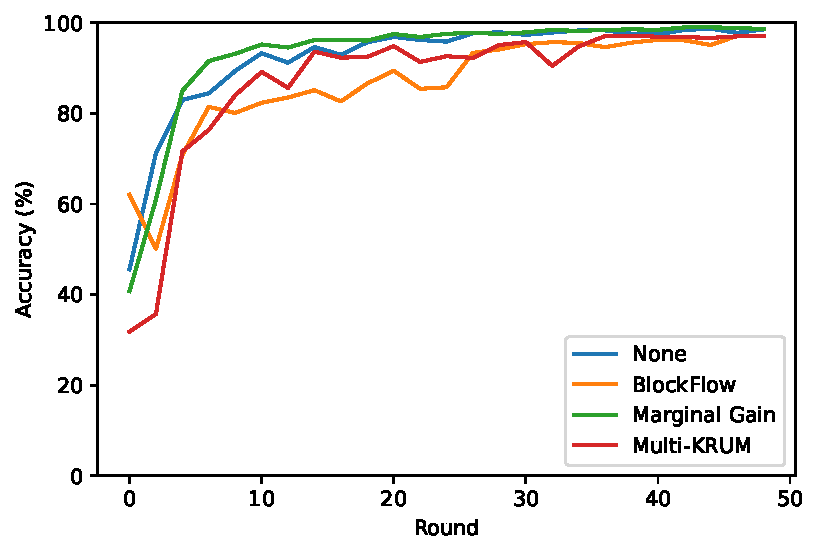
\includegraphics[width=0.7\textwidth]{graphics/scoring/accuracy.pdf}
    \caption{Model Accuracy Per Scoring Algorithm}
    \label{fig:accuracy_scoring}
\end{figure}

As it can be seen from \autoref{fig:accuracy_scoring}, all scoring algorithms reached a high model accuracy of at least  $97\%$. However, some algorithms reached higher accuracy values faster than others, that is, some converge faster. Overall, Marginal Gain converges the fastest, followed by no scoring, then by Multi-KRUM and lastly by BlockFlow.

The BlockFlow, is not only the slowest converging scoring algorithm, but also the only algorithm that does not reject submissions when aggregating, as explained in \Cref{background:scoring}. By not rejecting submissions, but still giving them a score to be used during the weighted aggregation, worse submissions are always included in the global model, which can lead to lower convergence rates. 

The Marginal Gain and Multi-KRUM algorithms both reject the worst submissions in each round and only consider the best. While the Marginal Gain uses its own score for the aggregation, the Multi-KRUM uses the number of samples of each submission, similar to the case when no scoring algorithm is used. For this reason, the Multi-KRUM algorithm convergence resembles the one of no scoring algorithm, while the Marginal Gain has a smoothest convergence curve.

\subsubsection{Communication Costs}

Communication costs also vary massively depending on which  scoring algorithm is used. Some place more strain on the clients, where others place more strain on the servers. \autoref{fig:net_scoring} presents the network traffic per round per scoring algorithm on the clients, servers, and blockchain processes.

\begin{figure}[!ht]
    \centering
    \centering
    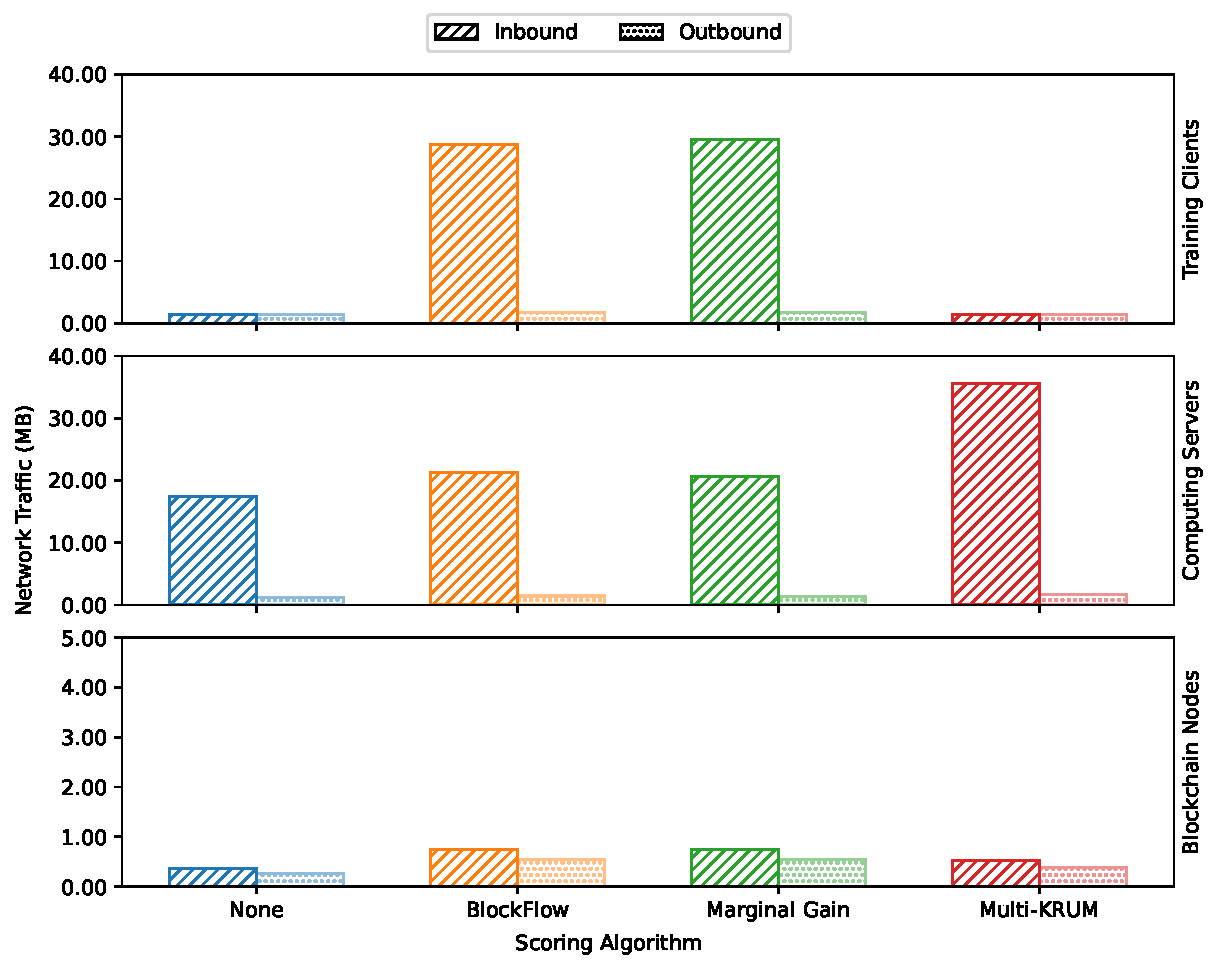
\includegraphics[width=0.8\textwidth]{graphics/scoring/net.pdf}
    \caption{Network Traffic Per Round Per Scoring Algorithm}
    \label{fig:net_scoring}
\end{figure}

Regarding the clients, there is a large difference in terms of the network traffic when comparing no scoring algorithm and the Multi-KRUM with the BlockFlow and Marginal Gain. On the one hand, the Multi-KRUM has similar traffic requirements to using no scoring algorithm on the clients because the scoring algorithm is executed on the servers. On the other hand, the BlockFlow and Marginal Gain have higher inbound traffic at the clients, while the outbound traffic remains similar. This can be explained by the fact that both BlockFlow and Marginal Gain algorithms are executed by the clients. Consequently, each client has to download the weights from all other clients in each round in order to calculate the score, leading to a higher inbound traffic.

Regarding the servers, there is not much difference between algorithms, except for the Multi-KRUM, which calculates the scores on the server. Therefore, the server downloads the weights of each client and requires additional time to calculate the scores, compared to the remaining algorithms that only download the weights once for the aggregation.

Finally, regarding the blockchain, we observe that when using the BlockFlow and Marginal Gain algorithms that there is a higher network traffic. The Multi-KRUM also requires more traffic than no scoring algorithm, but not as much as the BlockFlow or Marginal Gain. Since the number of clients is higher than the number of servers, there are more transactions when the scoring algorithm runs on the clients. When there are more transactions per round, there is more activity in the blockchain, leading to more network traffic per round.

\subsubsection{Computation Costs}

The computation costs across the servers and clients follow a similar trend to what we have seen with the communication costs. \autoref{fig:ram_scoring} and \autoref{fig:cpu_scoring} show the RAM and CPU usages on the client, server and blockchain processes, respectively.

Regarding the clients, all algorithms require similar amounts of RAM. The algorithms that run on the client, i.e., the Marginal Gain and BlockFlow, consume slightly more RAM, due to having more weights stored in memory, but the difference is negligible when compared to the total amount of RAM they consume. This can be explained by the fact that the weights are relatively small ($\approx 2$ MB) compared to the total RAM necessary to train a model. With respect to the CPU usage, it can be seen that the algorithms that run on the client, i.e., BlockFlow and Marginal Gain, have the lowest CPU idle time on the clients, while taking longer to be executed. This shows that calculating the scores on the client implies consistently higher CPU usage on the clients for longer periods of time.

Regarding the servers, it is clear that Multi-KRUM, being the only scoring algorithm that runs on the server, requires higher amount of RAM. However, the difference ($\approx 15$ MB) is not significant when considering that the servers have large amount of resources at their disposal. In addition, the Multi-KRUM also shows higher level of CPU usage, with frequent spikes to $100\%$.

Finally, regarding the blockchain, the difference of CPU and RAM usages among the different scoring algorithms is negligible. Even though the blockchain receives more transactions in total, it does not reflect on the RAM and CPU usage. The blockchain, by itself, already produces blocks at a constant rate. Therefore, the number of transactions required for the BFL system does not change significantly the CPU or RAM usage.

\begin{figure}[!hpt]
    \centering
    \centering
    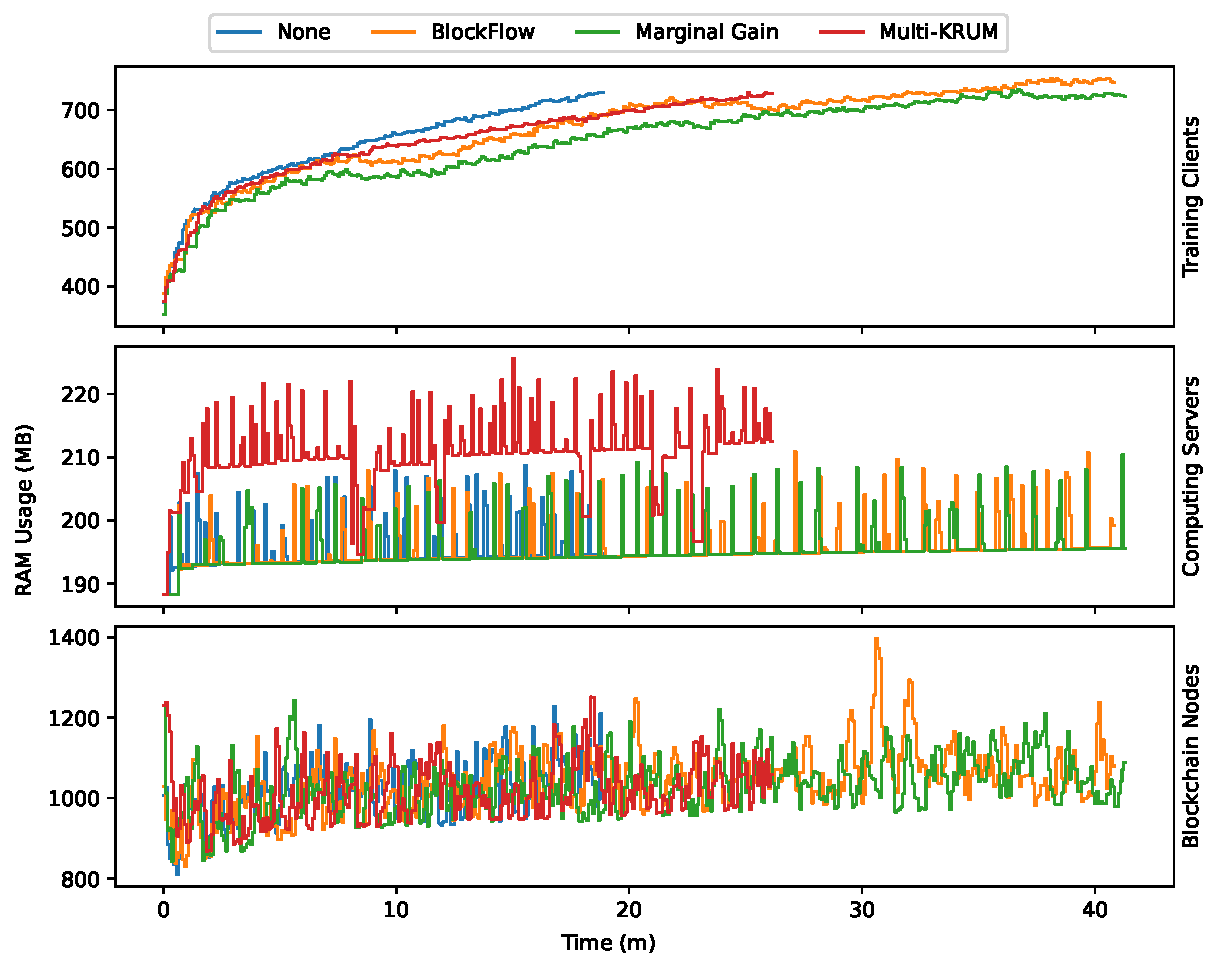
\includegraphics[width=0.8\textwidth]{graphics/scoring/ram.pdf}
    \caption{RAM Usage Per Scoring Algorithm}
    \label{fig:ram_scoring}
\end{figure}

\begin{figure}[!hpb]
    \centering
    \centering
    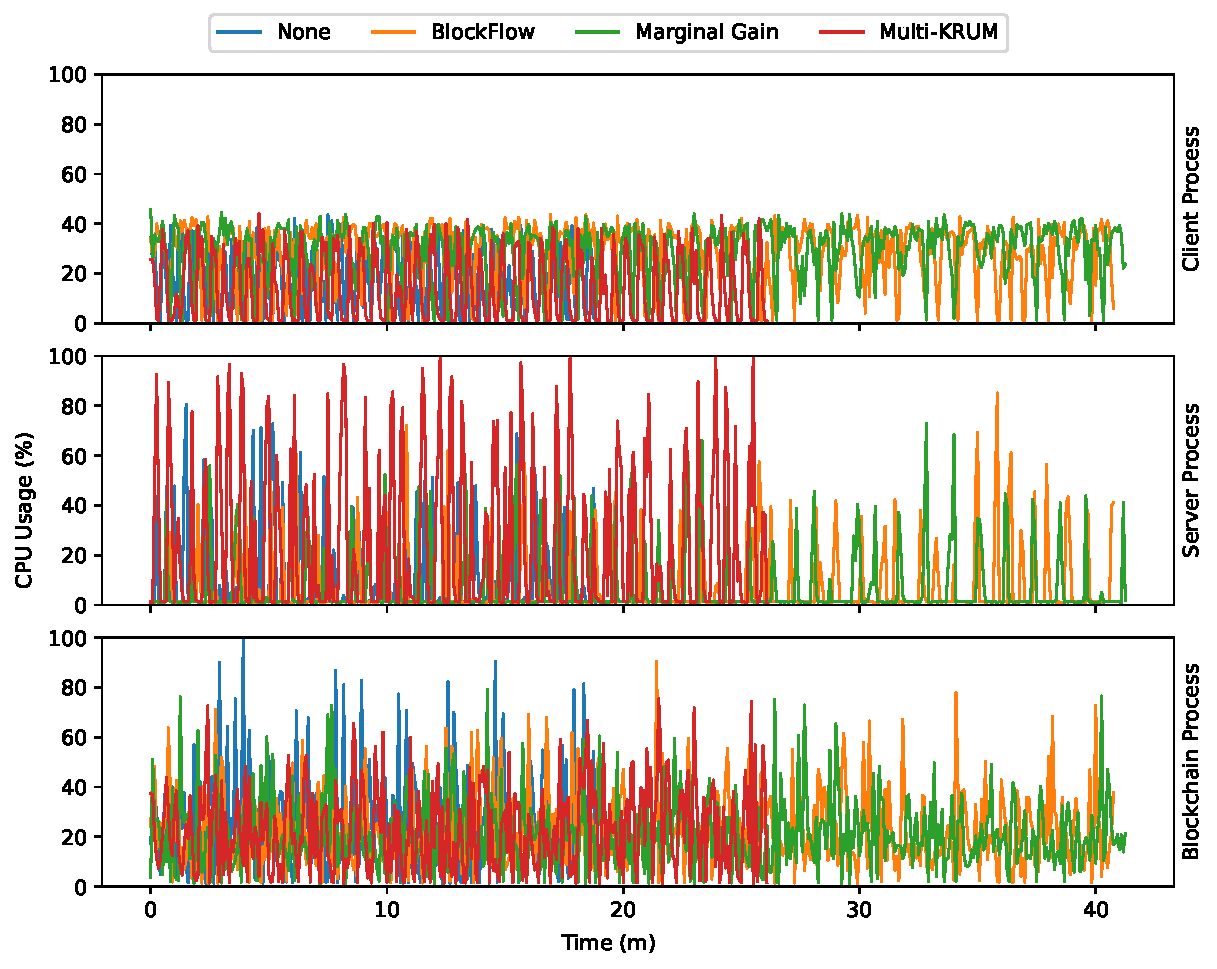
\includegraphics[width=0.8\textwidth]{graphics/scoring/cpu.pdf}
    \caption{CPU Usage Per Scoring Algorithm}
    \label{fig:cpu_scoring}
\end{figure}

\subsubsection{Conclusions and Improvements}

In conclusion, scoring algorithms that are executed on the clients, i.e.,the Marginal Gain and BlockFlow, have a higher impact on the overall system, leading to longer experiment execution times and higher resource usage for the clients. In contrary, algorithms that are executed on the servers, i.e., the Multi-KRUM, have a higher impact on the servers. Since there is usually a much higher number of clients than servers, the scoring algorithms executed by the servers have less impact on the overall system than the former. Additionally, the Marginal Gain was the most well performing algorithm in terms of model accuracy and convergence speed, followed by the Multi-KRUM and the BlockFlow.

If we had to choose an algorithm, the choices come down to the priorities of the system. If we are working with a system with resource-constrained devices, such as IoT systems, it is important that the impact on the clients is low. Therefore, scoring algorithms that run on the server, such as the Multi-KRUM, are more valuable. If the opposite is true, or if the resource consumption at the client is not relevant, the Marginal Gain could be chosen as it provides the best accuracy of the three.

It is also important to mention that algorithms that require more network traffic per round may be slower on clients with low bandwidth, which is the case of many IoT networks. With lower bandwidths, less traffic can go through at any point in time. Therefore, in case of high network traffic required during a round, devices with low bandwidth can make the process slower.

As a future improvement, servers can cache the client's update weights. Specifically, in case of the Multi-KRUM algorithm, the servers can download each of the client's submission twice: one time for scoring, one time for aggregating. However, the weights downloaded both times are the same as they are part of the same round. Therefore, caching can work well in favor of reducing the network traffic at the server for scoring algorithms that are executed by servers.

\subsection{Number of Clients}\label{horizontal:number_of_clients}

In this section, we analyze the impact of different numbers of clients on the scoring algorithms. For this comparison, all properties of the system are fixed, except for the amount of clients, which varies between 5, 10, 25 and 50, per each scoring algorithm.

\subsubsection{Execution Time, Transaction Cost, and Transaction Latency}

\autoref{fig:clients_metrics} illustrates the execution times, as well as the transaction latency and costs. The execution times of all scoring algorithms increase with the number of clients. However, they do not increase the same way. The Multi-KRUM algorithm, as well as not using any scoring algorithm, have a smaller execution time increase with the number of clients, when compared to BlockFlow and Marginal Gain. This can be explained by the fact that, in BlockFlow and Marginal Gain, the scorers are the clients. Since, as previously discussed, there are more clients than servers, the smart contract has to wait for more scorers to submit their scores, than it would have to wait when using Multi-KRUM. Consequently, the execution time increase with the number of devices is higher with scoring algorithms executed by the clients.

\begin{figure}[!ht]
    \centering
    \begin{subfigure}[b]{0.49\textwidth}
        \centering
        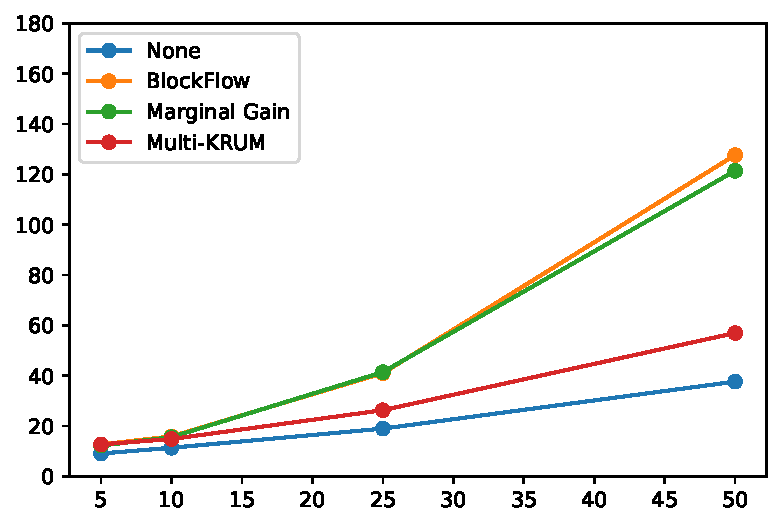
\includegraphics[width=\textwidth]{graphics/clients/e2e.pdf}
        \caption{E2E Time}
    \end{subfigure}
    \hfill
    \begin{subfigure}[b]{0.49\textwidth}
        \centering
        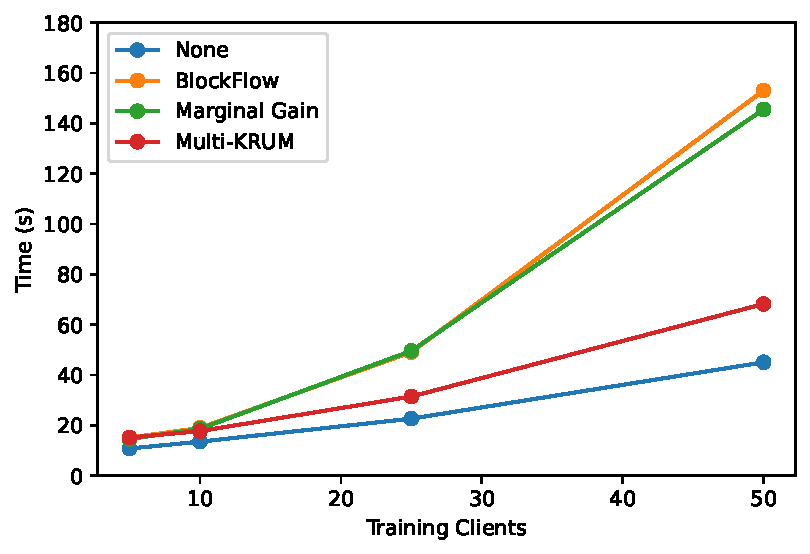
\includegraphics[width=\textwidth]{graphics/clients/round.pdf}
        \caption{Mean Round Time}
    \end{subfigure}
    \hfill
    \begin{subfigure}[b]{0.49\textwidth}
        \centering
        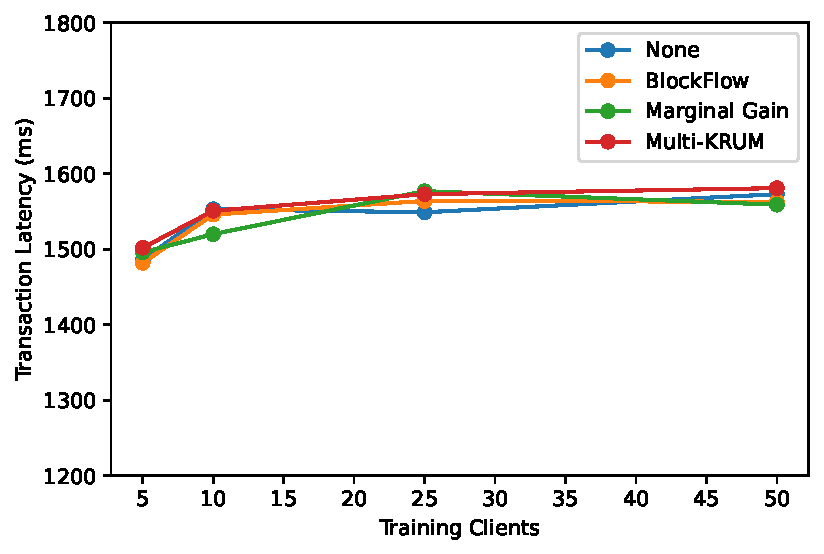
\includegraphics[width=\textwidth]{graphics/clients/tx_latency.pdf}
        \caption{Mean Transaction Latency}
    \end{subfigure}
    \hfill
    \begin{subfigure}[b]{0.49\textwidth}
        \centering
        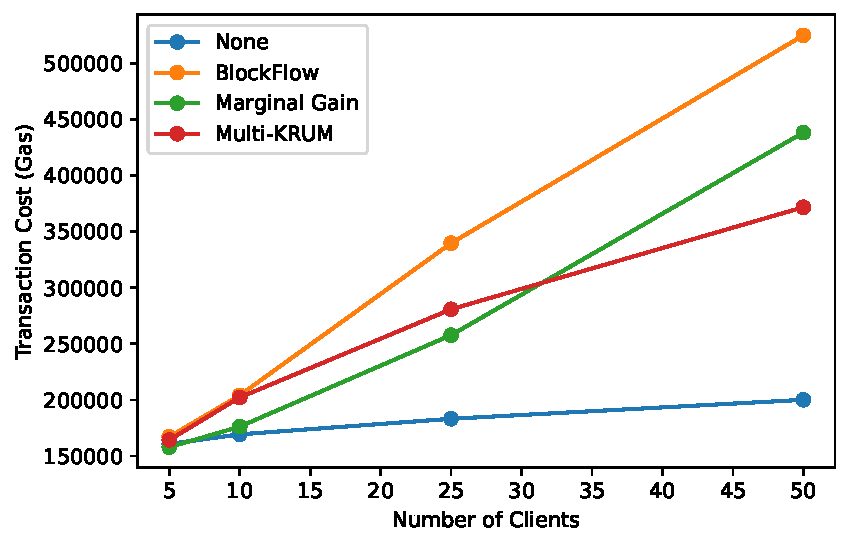
\includegraphics[width=\textwidth]{graphics/clients/tx_cost.pdf}
        \caption{Mean Transaction Cost}
    \end{subfigure}
    \caption{Execution Time, Transaction Cost, and Transaction Latency Per Number of Clients}
    \label{fig:clients_metrics}
\end{figure}

Regarding the transaction latency, there is no significant change with the variation of number of clients. As discussed before, transaction latency is mostly determined by the capacity of the network to handle the transactions. The Ethereum has a relatively fixed capacity of transactions per second of around 15 transactions per second. Our system alone does not reach that rate of transactions, not influencing the transaction latency. It is worth pointing out that, if the number of clients was in the order of hundreds, leading to elevated number of transactions, the latency would likely increase.

Regarding the transaction costs, we observe that they increase with the increased number of clients. In addition, the transaction costs growth is similar per algorithm. Firstly, we can calculate how many transactions we incur per algorithm per round by $T+A+S$, where $T$ is the number of trainers, usually clients, $A$ is the number of aggregators, usually servers, and $S$ the number of scorers, which can be either the clients or servers. When no scoring algorithm is used, the system only requires $T+A$ transactions, where $T$ is the number of clients and the only growing variable. With the Multi-KRUM, the system requires $T+2A$ transactions, since $S=A$, leading to a faster growth than when no scoring algorithm is used. Finally, both BlockFlow and Marginal Gain algorithms require $2T+A$ transactions and since $T > A$ and $T$ is the number of growing clients, it is also expected that the transaction cost would increase more than for the Multi-KRUM.

\subsubsection{Model Accuracy and Convergence}

As it can be seen from \autoref{fig:accuracy_clients}, the model accuracy and how it converges varies differently with different scoring algorithms. Overall, we observe that lower number of clients leads to a less stable convergence, represented by the spiking in the model accuracy plots. With a low number of clients, such as 5, the selected number of clients per round is also low due to the random way the participant selection algorithms chooses how many clients participate per round. Therefore, the model is trained with less diverse data per round. Consequently, the model can skew at some points during training, leading to a less stable convergence. In contrary, using more clients, namely 25 and 50, has an overall positive effect on both convergence stability and convergence speed. This is also likely related to the fact that the model is trained with more diverse samples from more clients in each round, leading to a better results.

\begin{figure}[!ht]
    \centering
    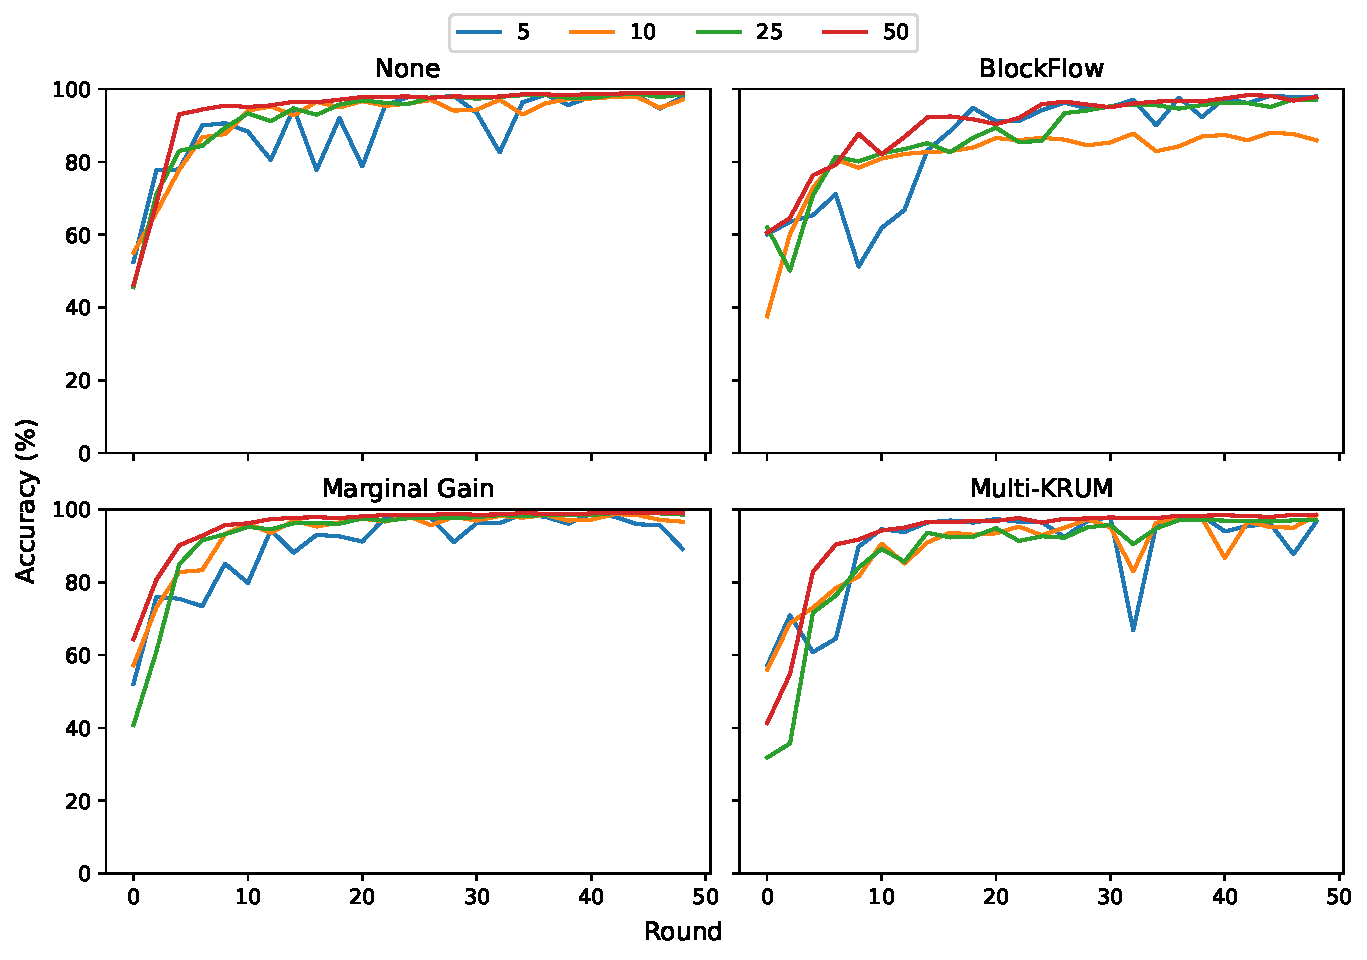
\includegraphics[width=\textwidth]{graphics/clients/accuracy.pdf}
    \caption{Model Accuracy Per Number of Clients}
    \label{fig:accuracy_clients}
\end{figure}

When it comes to the algorithm that performs best, the conclusions drawn from \Cref{horizontal:scoring_overall} remain true: the Marginal Gain performs the best, followed by the Multi-KRUM and finally by the BlockFlow.

\subsubsection{Communication Costs}

As it can be seen from \autoref{fig:net_clients}, the communication costs vary with the number of clients. Firstly, we observe that in terms of incoming traffic at the client process, there are significant differences depending on the scoring algorithm used.

\begin{figure}[!ht]
    \centering
    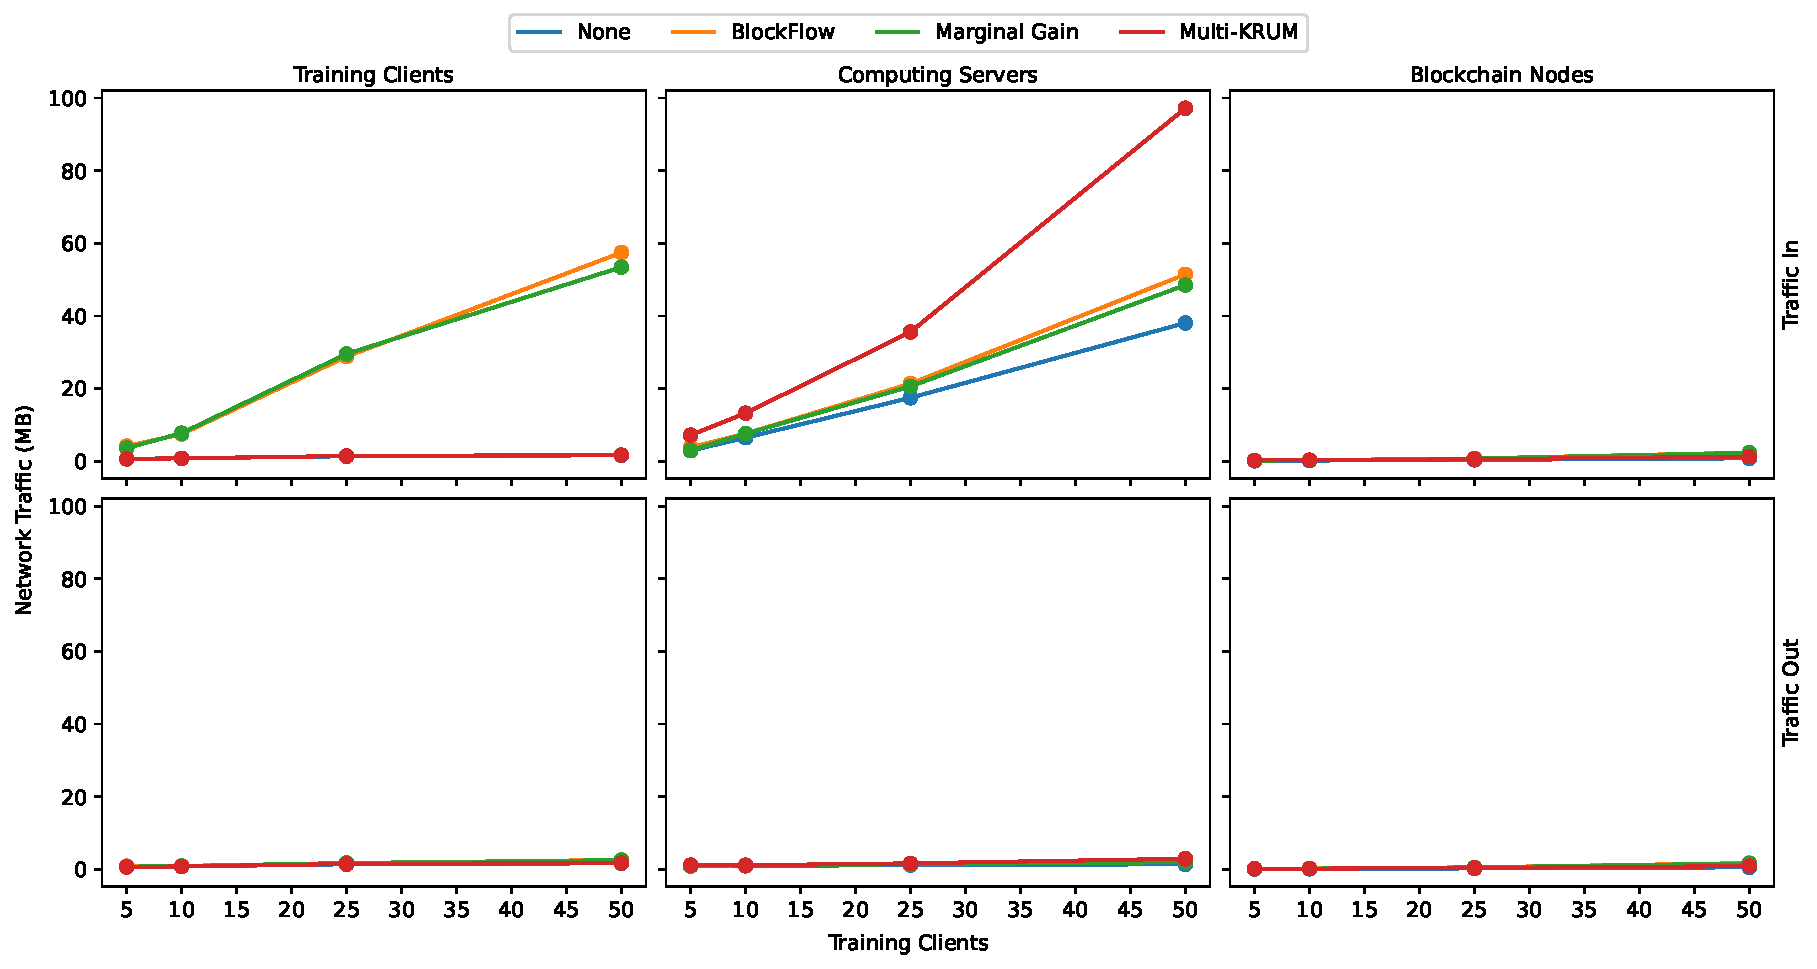
\includegraphics[width=\textwidth]{graphics/clients/traffic.pdf}
    \caption{Network Traffic Per Number of Clients}
    \label{fig:net_clients}
\end{figure}

One may notice that incoming traffic at the clients only increases when using scoring algorithms that are executed by the clients, such as the BlockFlow and the Marginal Gain. This can be explained by the fact that the more clients means the more weights from these clients need to be downloaded and scored. In contrary, when the scoring algorithm is executed by the server, there are virtually no changes in the incoming traffic when number of clients is increased. This is because the client only has to download the global weights after each round, which is not influenced by the number of clients.

Secondly, we observe that the incoming traffic always grows linearly at the servers when using a scoring algorithm that runs at the clients. However, when using a algorithm that runs on the server, such as the Multi-KRUM, the growth is higher than for the remaining algorithms. In all cases, the servers always have to download the weights for aggregation. However, if the scoring is executed at the servers, they will download the weights twice as explained in \Cref{horizontal:scoring_overall}, leading to a super-linear traffic growth. As previously suggested, this can be improved by caching the weights between these two phases.

Thirdly, we observe that the outgoing traffic differences are not significant for any of the processes. Regarding the clients and servers, we observe a very small increase on the client or server processes, if the scoring algorithm is executed by the clients or servers, respectively. However, the differences of outgoing traffic per number of clients for each scoring algorithm are negligible.

Finally, the differences observed in the blockchain process, both for incoming and outgoing traffic are negligible. With the increase of the number of clients, there are more transactions going through the blockchain. However, the transactions on the blockchain are very small when compared to the size of weights that need to be uploaded and downloaded by the clients and servers, respectively.

\subsubsection{Computation Costs}

\autoref{fig:ram_clients_clients}, \autoref{fig:ram_clients_servers}, \autoref{fig:ram_clients_miners} show the RAM usage at the clients, servers, and blockchain processes, while  \autoref{fig:cpu_clients_clients}, \autoref{fig:cpu_clients_servers}, \autoref{fig:cpu_clients_miners} show the CPU usage at the clients, servers, and blockchain processes, respectively. Overall, it can be seen that the number of clients has no major impact on RAM and CPU usage of either clients or servers.

Even though the usage of RAM and CPU at a certain points in time does not vary significantly, some scoring algorithms have more impact on the clients, or on the servers, as discussed in \Cref{horizontal:scoring_overall}. In addition, we observe that the increase of resource usage is proportional to the number of clients, depending on whether the the scoring algorithm is executed by the clients or the servers.

The only major change is observed in the RAM and CPU usage of the blockchain process. The higher the number of clients, the higher the RAM and CPU usage. This is expected as more clients are connected to the blockchain, meaning that more devices continuously interact and send transactions to the blockchain.

\subsubsection{Conclusions and Improvements}

In conclusion, scoring algorithms executed by the clients, i.e., the BlockFlow and Marginal Gain, show higher execution time increases with respect to the number of clients. In addition, the resource usage at the clients increases linearly with the number of devices. In contrary, algorithms executed by the servers, i.e., the Multi-KRUM, do not have significant effects on the clients' resources usage. Therefore, in systems with resource-constrained clients, algorithms executed by the server may be the ideal solution.

Finally, the resource usage of the blockchain process, mainly in terms of RAM, increases with the number of clients. The blockchain resource usage is an important aspect to consider in BFS systems. There is a clear trade-off between the number of clients with the blockchain resource usage.

\subsection{Privacy Degrees}

In this section, we analyze the impact of different privacy degrees on each scoring algorithm. In this set of experiments, all properties of the system are fixed, except for the degree of privacy, which varies between 0, 1 and 5, per each scoring algorithm.

\subsubsection{Execution Time, Transaction Cost, and Transaction Latency}

As it can be seen from \autoref{fig:priv_metrics}, having a privacy mechanism increases the execution time of each round by approximately $16.6$ seconds. In addition, the privacy degree itself does not seem to influence the execution time significantly.

Regarding the transaction latency and costs, there are no significant differences. The privacy mechanism is executed by the clients before they submit their model update, and does not change the number of transactions. Consequently, it has no impact on the blockchain process itself.

\begin{figure}[!hpt]
    \centering
    \begin{subfigure}[b]{0.47\textwidth}
        \centering
        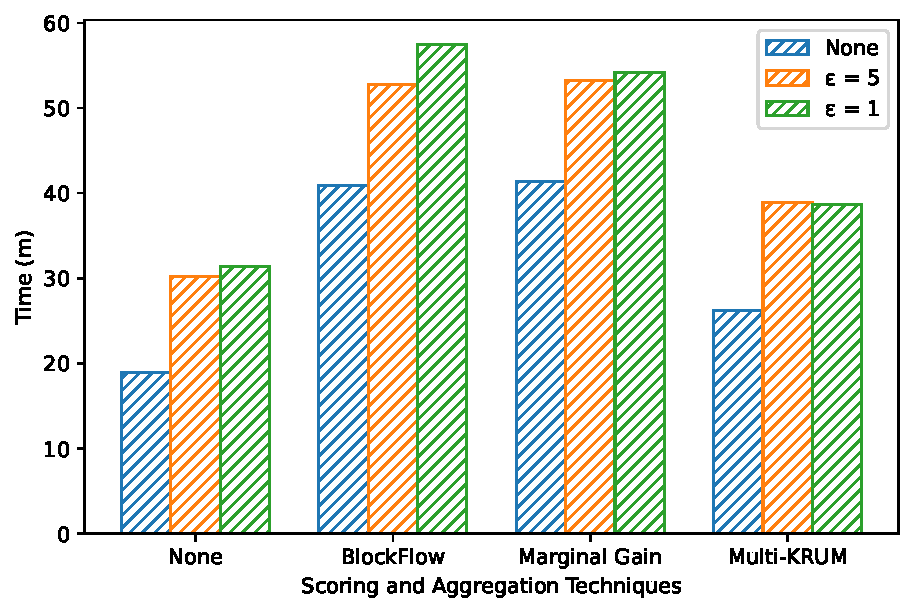
\includegraphics[width=\textwidth]{graphics/privacy/e2e.pdf}
        \caption{E2E Time}
    \end{subfigure}
    \hfill
    \begin{subfigure}[b]{0.47\textwidth}
        \centering
        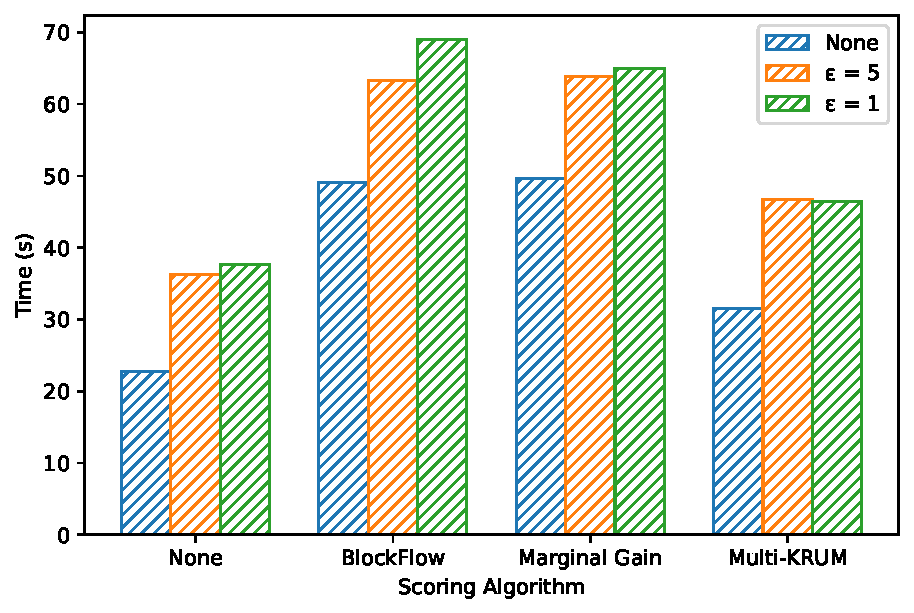
\includegraphics[width=\textwidth]{graphics/privacy/round.pdf}
        \caption{Mean Round Time}
    \end{subfigure}
    \hfill
    \begin{subfigure}[b]{0.47\textwidth}
        \centering
        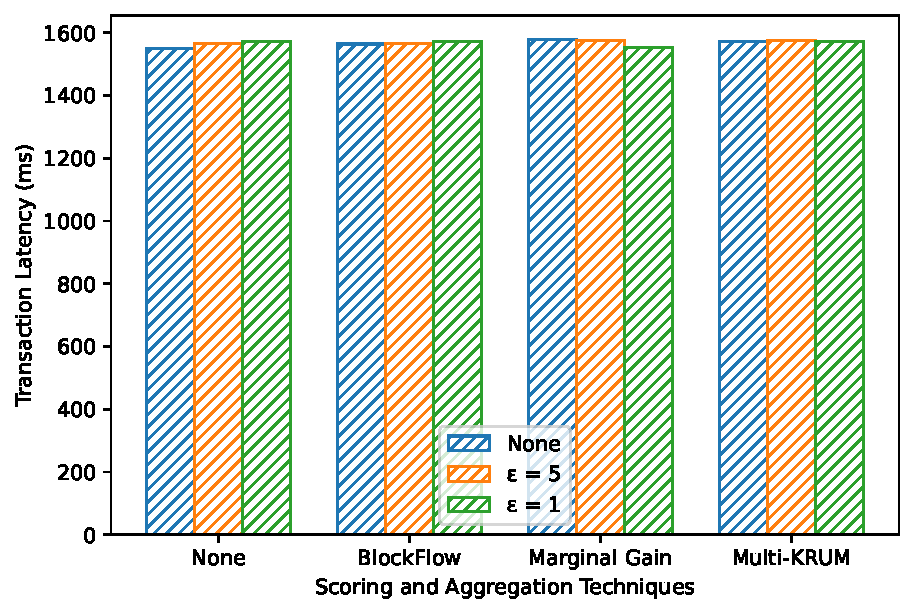
\includegraphics[width=\textwidth]{graphics/privacy/tx_latency.pdf}
        \caption{Transaction Latency}
    \end{subfigure}
    \hfill
    \begin{subfigure}[b]{0.47\textwidth}
        \centering
        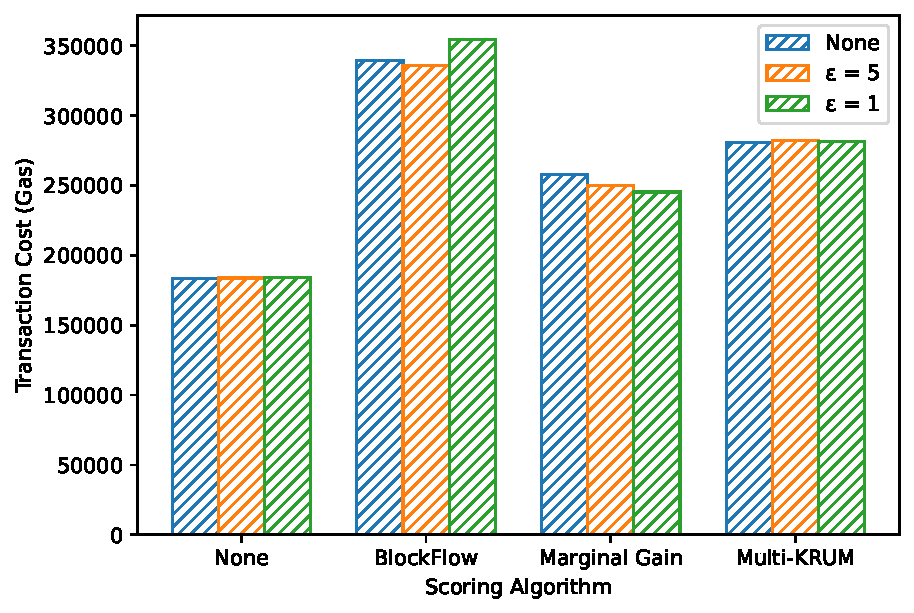
\includegraphics[width=\textwidth]{graphics/privacy/tx_cost.pdf}
        \caption{Transaction Cost}
    \end{subfigure}
    \caption{Execution Time, Transaction Cost, and Transaction Latency Per Privacy Degree}
    \label{fig:priv_metrics}
\end{figure}

\begin{figure}[!hpb]
    \centering
    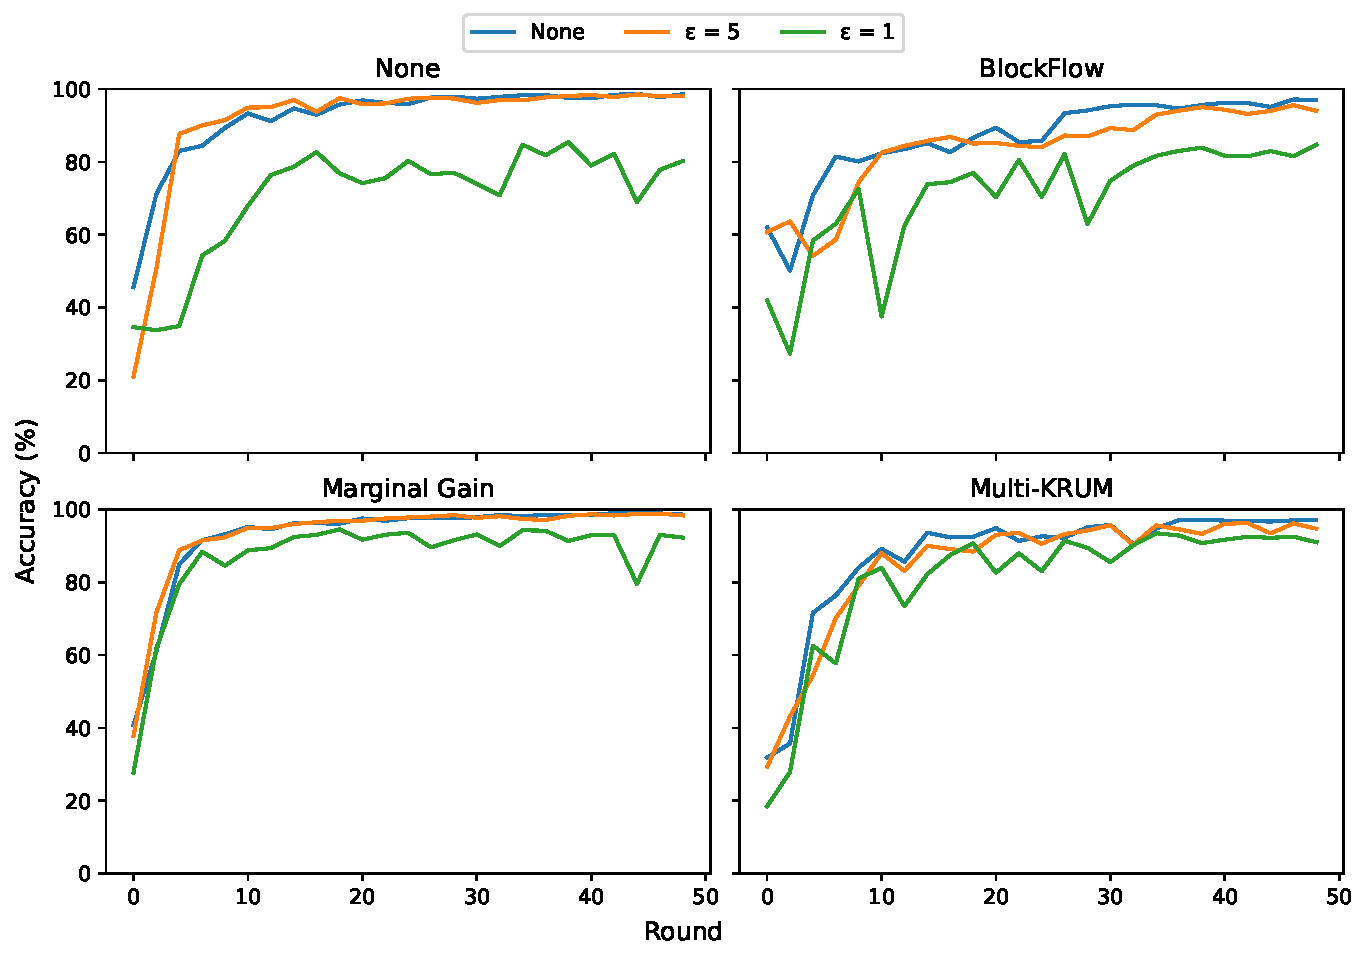
\includegraphics[width=\textwidth]{graphics/privacy/accuracy.pdf}
    \caption{Model Accuracy Per Privacy Degree}
    \label{fig:accuracy_privacy}
\end{figure}

\subsubsection{Model Accuracy and Convergence}

As it can be seen from \autoref{fig:accuracy_privacy}, different scoring algorithms have different accuracy drops using different privacy degrees. Overall, we observe that not using a scoring algorithm performs the worse with the highest degree of privacy, i.e., $\epsilon = 1$. In addition, a lower degree of privacy, i.e., $\epsilon = 5$, yields similar, yet lower, model accuracy than not using privacy degree. The higher the degree of privacy, the higher the noise values that are added to the original weights. Since the weights include added noise, it is expected that the accuracy will be lower with the higher degrees of privacy.

Out of the three scoring algorithms, the Marginal Gain and Multi-KRUM perform the best in presence of the higher degrees of privacy. As explained in \Cref{background:scoring}, both of these algorithms reject the worst updates, while BlockFlow does not. By rejecting the worst update, these algorithms always keep the best updates that provide the higher accuracy, even after noise is being added to the weights. Therefore, the Multi-KRUM and Marginal Gain have a lower accuracy drop with the higher privacy degrees, allowing them to maintain high model accuracy while preserving privacy.

\subsubsection{Communication Costs}

In terms of communication costs, as illustrated in \autoref{fig:net_privacy}, there are no significant differences depending on the privacy degree used. Adding noise to the weights does not necessarily increase their sizes and, for that reason, the network traffic costs are not expected to change significantly.

\begin{figure}[!h]
    \centering
    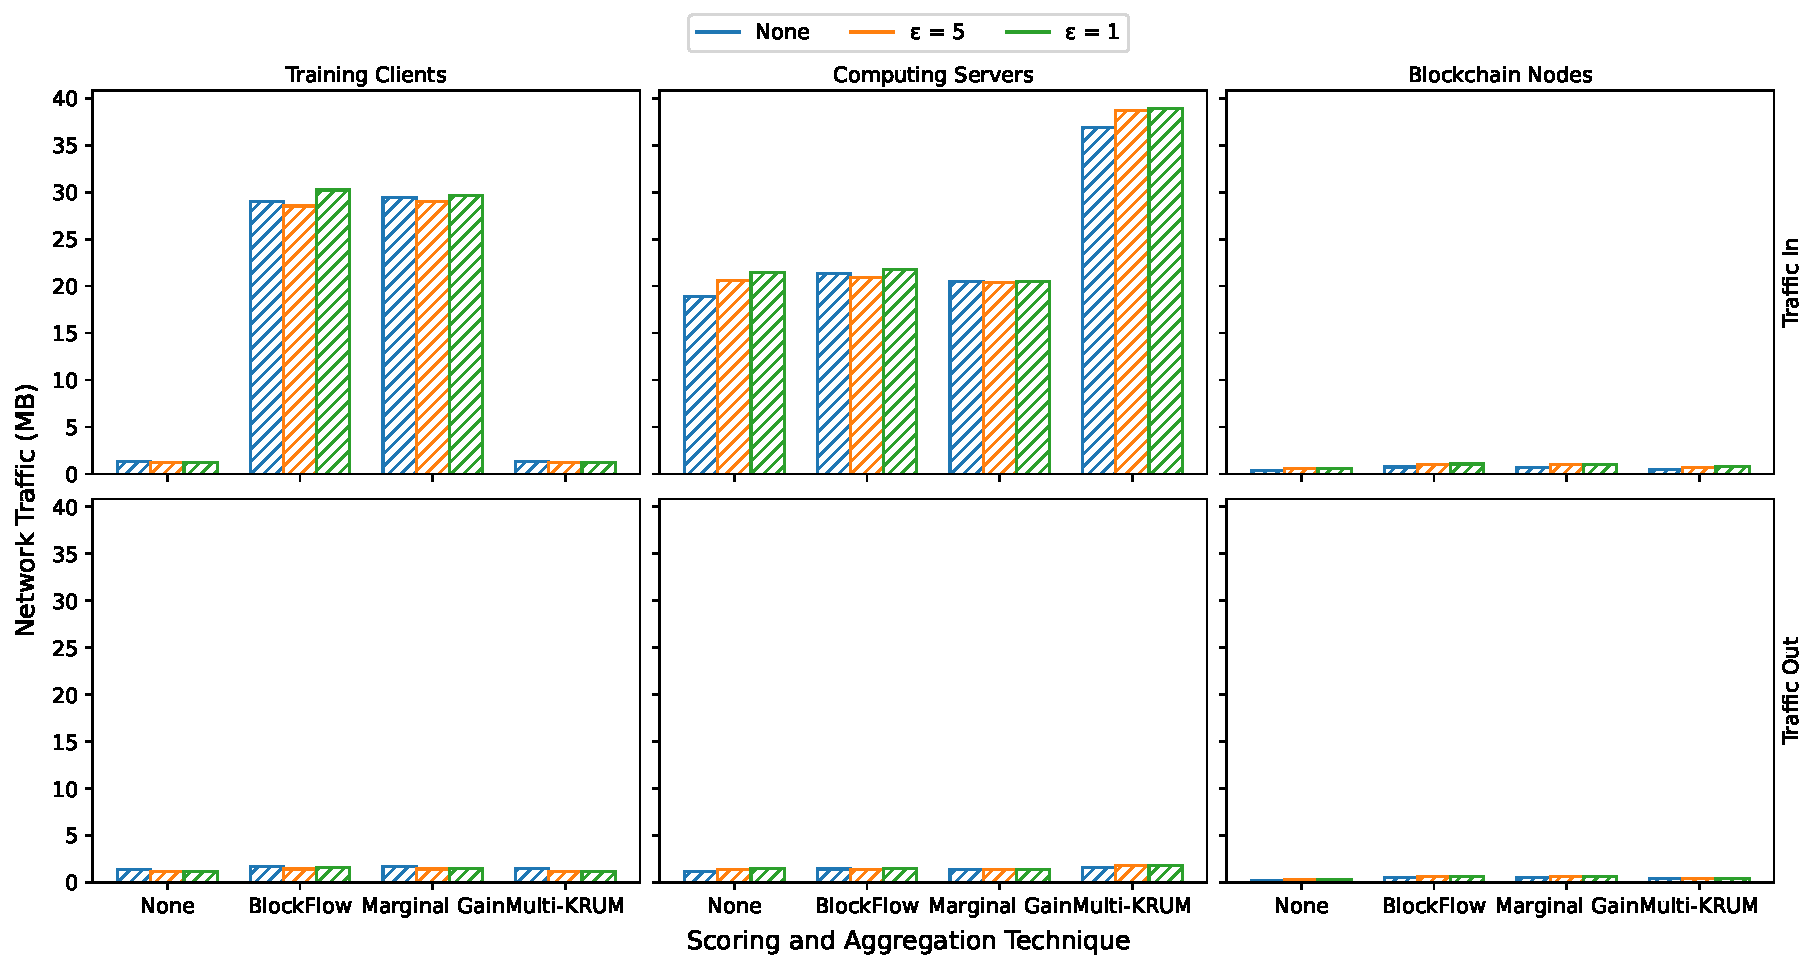
\includegraphics[width=\textwidth]{graphics/privacy/traffic.pdf}
    \caption{Network Traffic Per Privacy Degree}
    \label{fig:net_privacy}
\end{figure}

\subsubsection{Computation Costs}

\autoref{fig:ram_privacy_clients}, \autoref{fig:ram_privacy_servers}, \autoref{fig:ram_privacy_miners} show the RAM usage at the clients, servers, and blockchain processes, while \autoref{fig:cpu_privacy_clients}, \autoref{fig:cpu_privacy_servers}, \autoref{fig:cpu_privacy_miners} show the CPU usage at the clients, servers, and blockchain processes, respectively. Since the privacy algorithm is only executed by the client process, we only expect the computation costs, namely the CPU usage, to increase at the client process. Overall, we can observe that this is true as there are no significant changes in the RAM or CPU usage for the servers and blockchain processes.

As it can be seen from \autoref{fig:ram_privacy_clients}, the privacy mechanisms have no significant impact on RAM usage. The privacy algorithm has little RAM usage when compared to the total required for model training. In contrary, the CPU usage is higher, not necessarily in terms of usage percentage, but in terms of longer usage times. This can be seen from \autoref{fig:cpu_privacy_clients} and is explained by the time required for the execution of the privacy algorithm at the clients.

\subsubsection{Conclusions}

In conclusion, we see that using a privacy algorithm increases the computation costs, and consequently, the resource usage, at the clients. This leads to longer execution times as clients that need to process their weights and add noise to them. Therefore, there is a clear trade-off between execution time and privacy. However, increasing the privacy degree does not increase the execution time.

In addition, one may notice that increasing the privacy degree leads to the lower model accuracy. This is expected since the privacy algorithm used introduce noise to the weights. However, some of the scoring algorithms are still able to achieve higher model accuracy values even with higher privacy degrees. This is the case for the Marginal Gain and Multi-KRUM, which are the most well-performing algorithms.

Finally, we can argue that adding a privacy preserving algorithm to a BFS system is crucial, specially if the model is trained with sensitive data. One of the main arguments to apply blockchain to a Federated Learning system is the traceability and auditability. To do so, the weights, or their representation in our case, are recorded in the blockchain, which means they are visible and retrievable by anyone in the network. This implies that there is a trade-off between traceability and auditability and the requirement for privacy mechanisms, which in turn leads to higher resource usage.

\clearpage

\begin{figure}[!h]
    \centering
    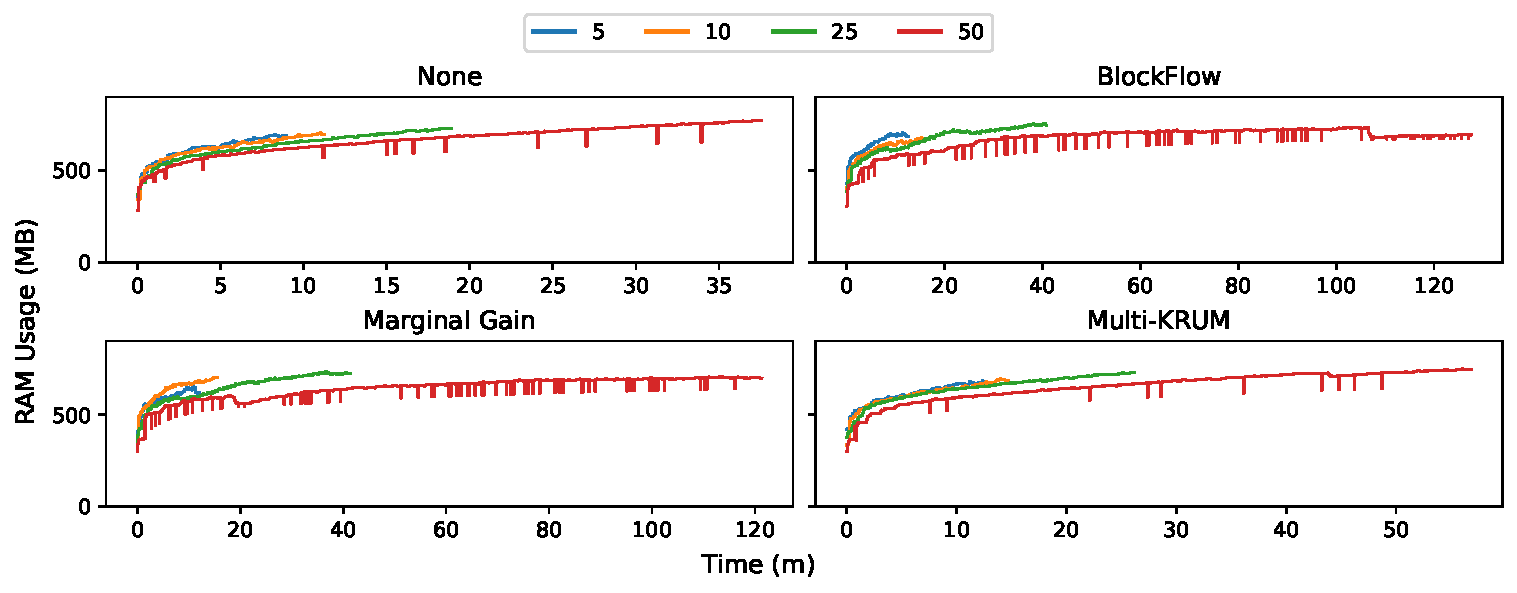
\includegraphics[width=\textwidth]{graphics/clients/ram_client.pdf}
    \caption{Client Process RAM Usage Per Number of Clients}
    \label{fig:ram_clients_clients}
\end{figure}

\vfill

\begin{figure}[!h]
    \centering
    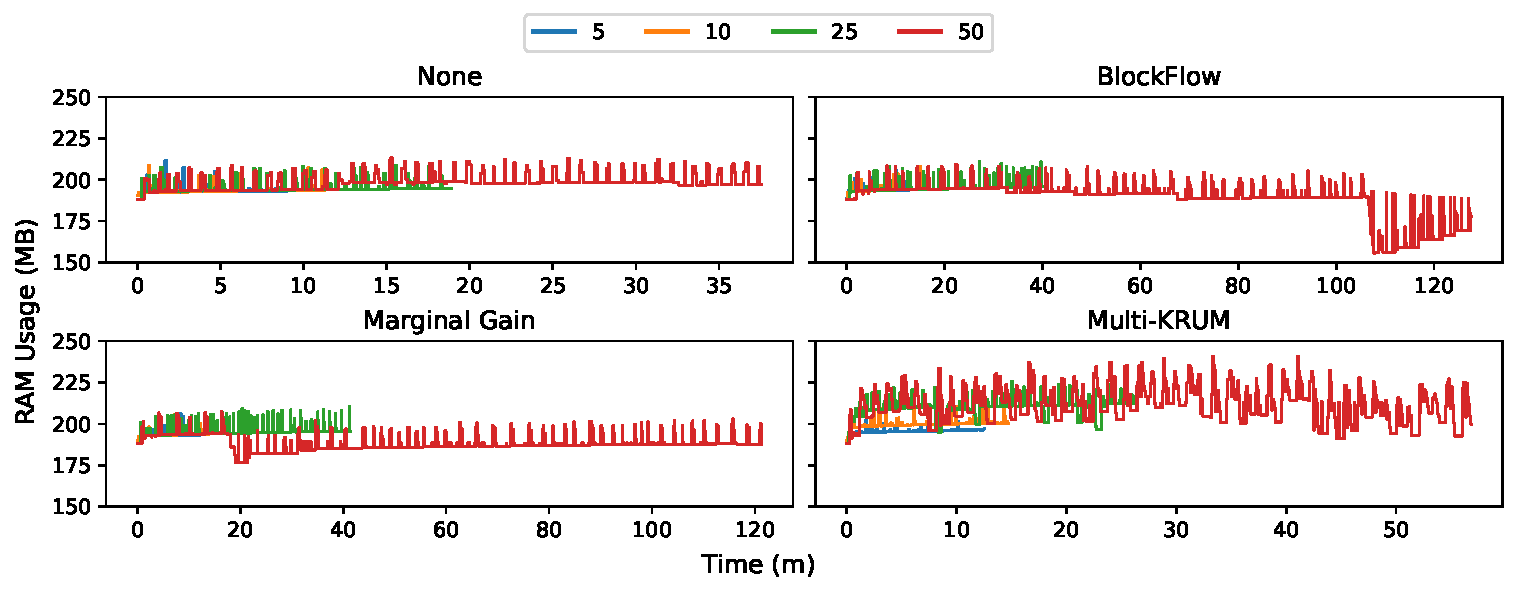
\includegraphics[width=\textwidth]{graphics/clients/ram_server.pdf}
    \caption{Server Process RAM Usage Per Number of Clients}
    \label{fig:ram_clients_servers}
\end{figure}

\vfill

\begin{figure}[!h]
    \centering
    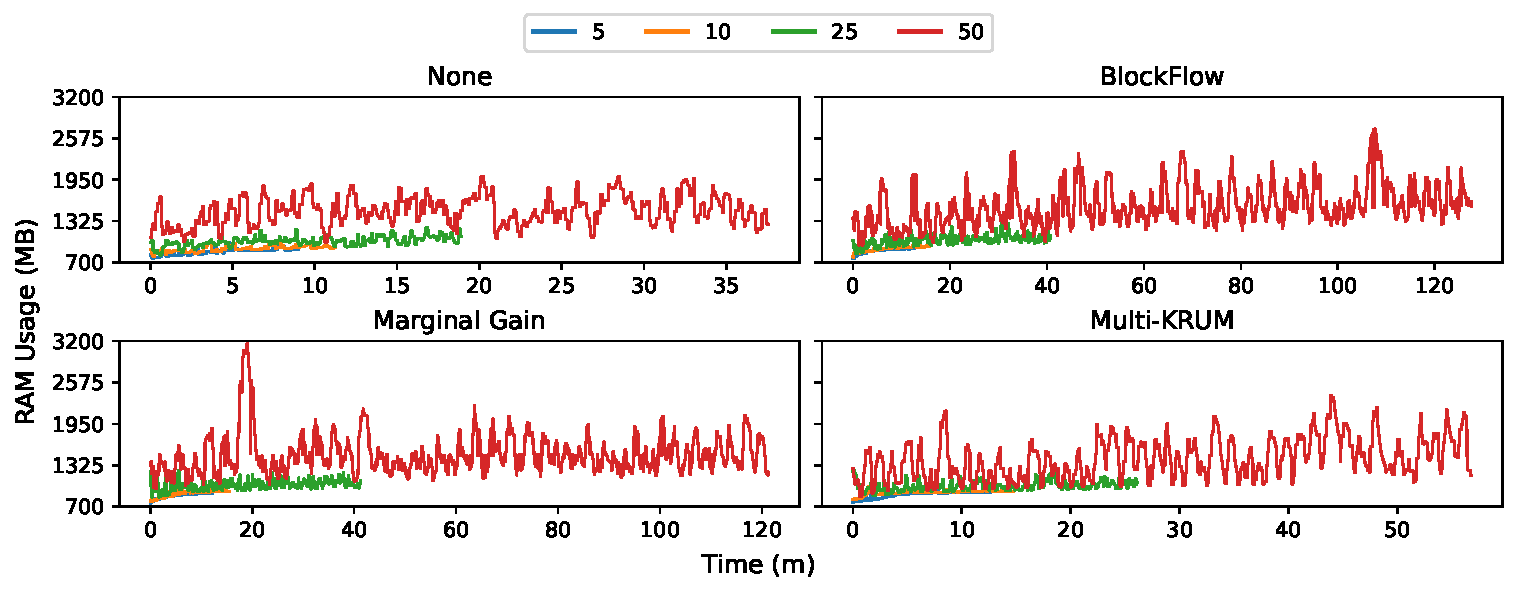
\includegraphics[width=\textwidth]{graphics/clients/ram_miner.pdf}
    \caption{Blockchain Process RAM Usage Per Number of Clients}
    \label{fig:ram_clients_miners}
\end{figure}

\clearpage

\begin{figure}[!h]
    \centering
    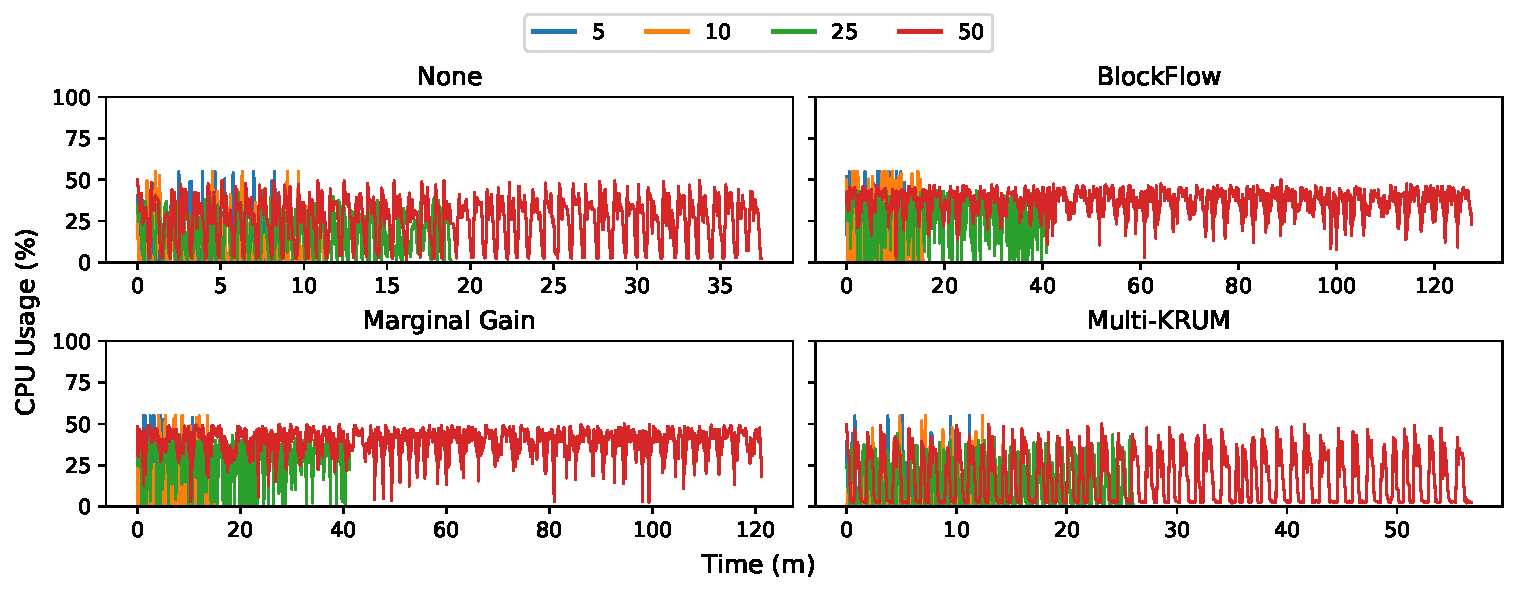
\includegraphics[width=\textwidth]{graphics/clients/cpu_client.pdf}
    \caption{Client Process CPU Usage Per Number of Clients}
    \label{fig:cpu_clients_clients}
\end{figure}

\vfill

\begin{figure}[!h]
    \centering
    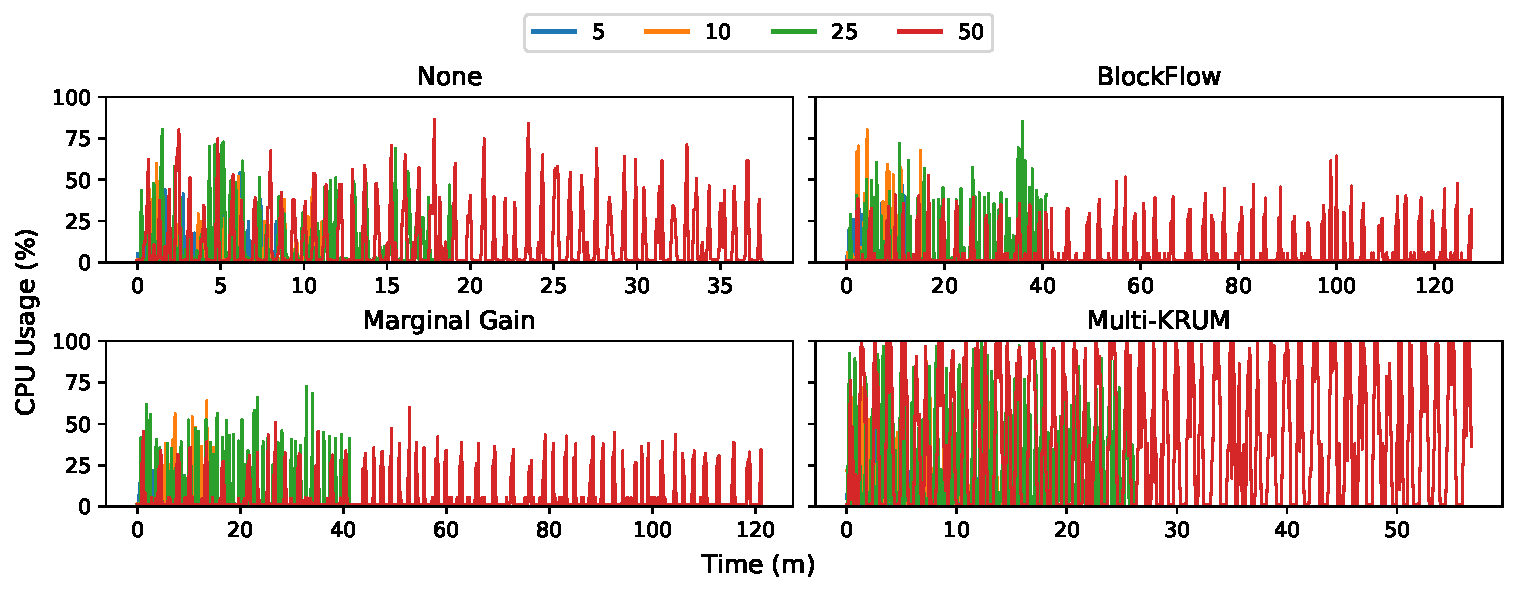
\includegraphics[width=\textwidth]{graphics/clients/cpu_server.pdf}
    \caption{Server Process CPU Usage Per Number of Clients}
    \label{fig:cpu_clients_servers}
\end{figure}

\vfill

\begin{figure}[!h]
    \centering
    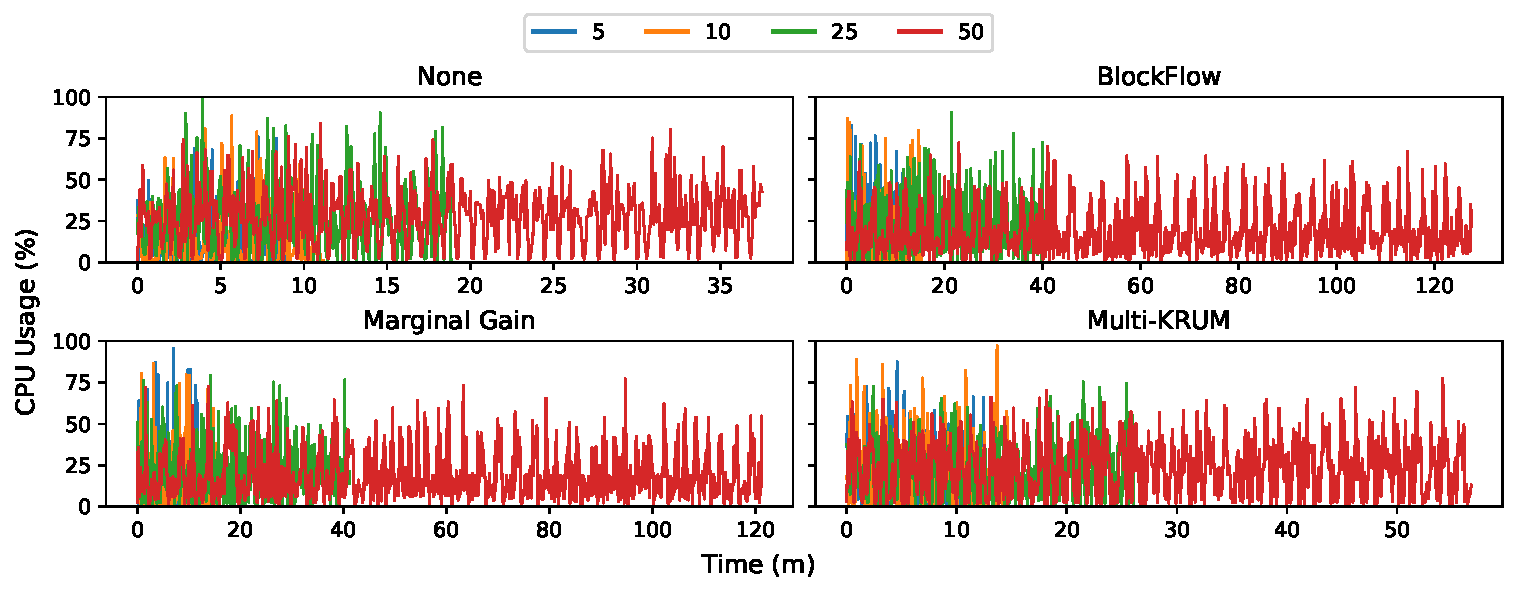
\includegraphics[width=\textwidth]{graphics/clients/cpu_miner.pdf}
    \caption{Blockchain Process CPU Usage Per Number of Clients}
    \label{fig:cpu_clients_miners}
\end{figure}

\clearpage

\begin{figure}[!h]
    \centering
    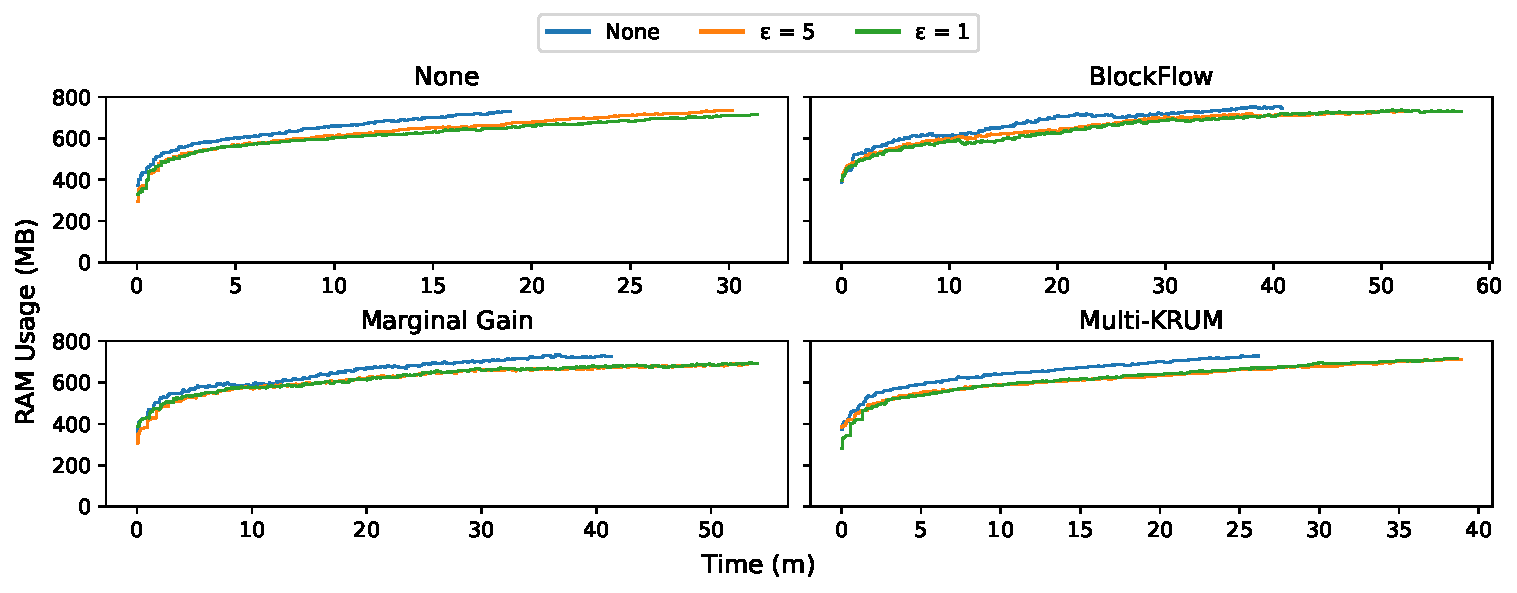
\includegraphics[width=\textwidth]{graphics/privacy/ram_client.pdf}
    \caption{Client Process RAM Usage Per Privacy Degree}
    \label{fig:ram_privacy_clients}
\end{figure}

\vfill

\begin{figure}[!h]
    \centering
    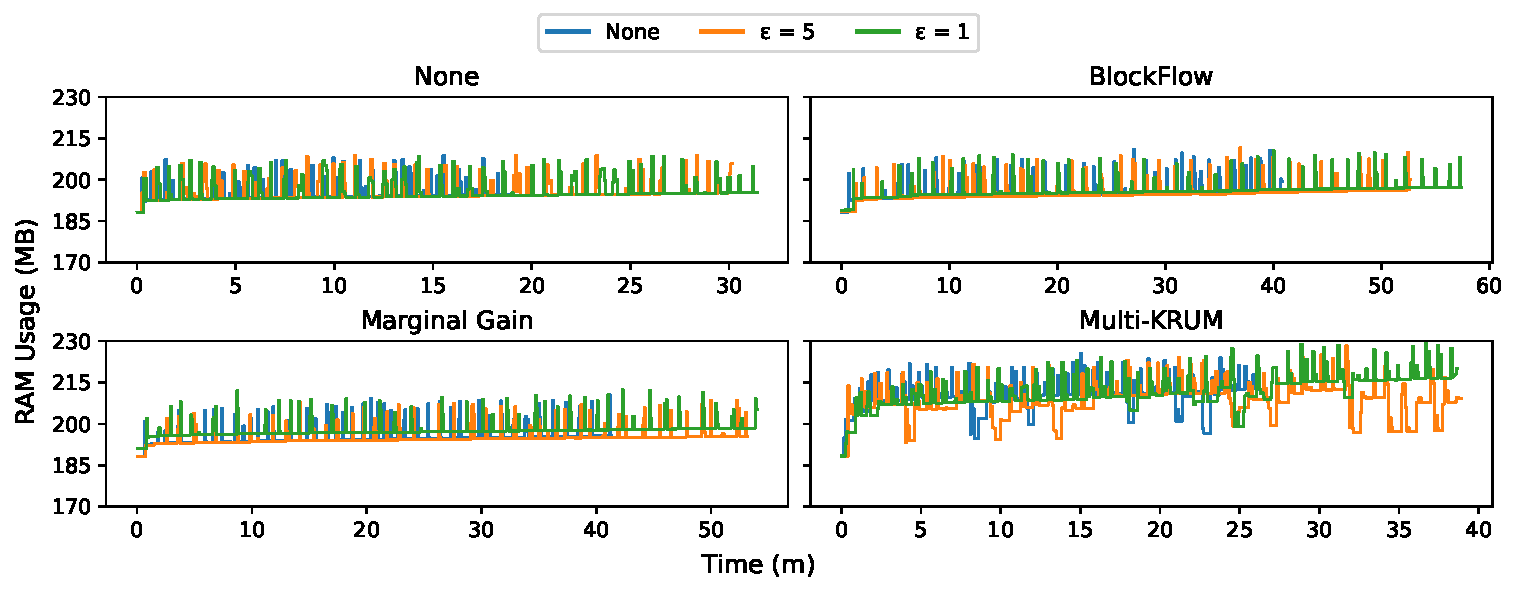
\includegraphics[width=\textwidth]{graphics/privacy/ram_server.pdf}
    \caption{Server Process RAM Usage Per Privacy Degree}
    \label{fig:ram_privacy_servers}
\end{figure}

\vfill

\begin{figure}[!h]
    \centering
    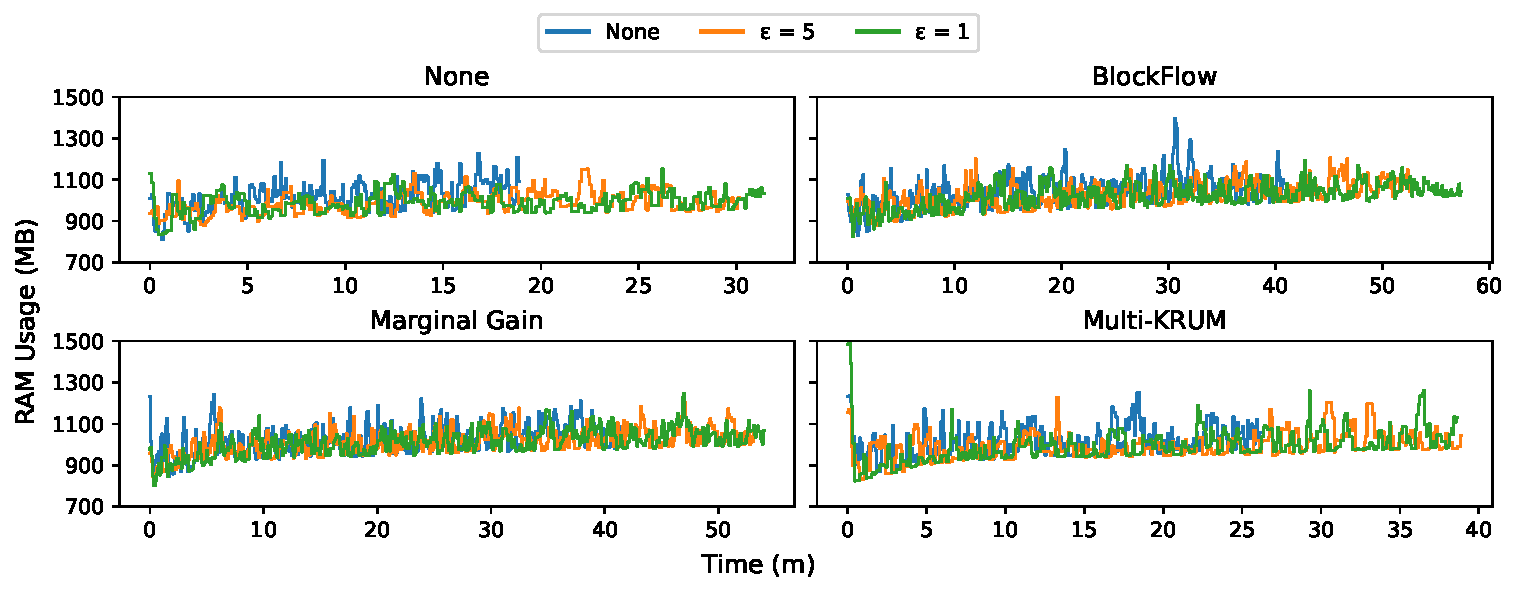
\includegraphics[width=\textwidth]{graphics/privacy/ram_miner.pdf}
    \caption{Blockchain Process RAM Usage Per Privacy Degree}
    \label{fig:ram_privacy_miners}
\end{figure}

\clearpage

\begin{figure}[!h]
    \centering
    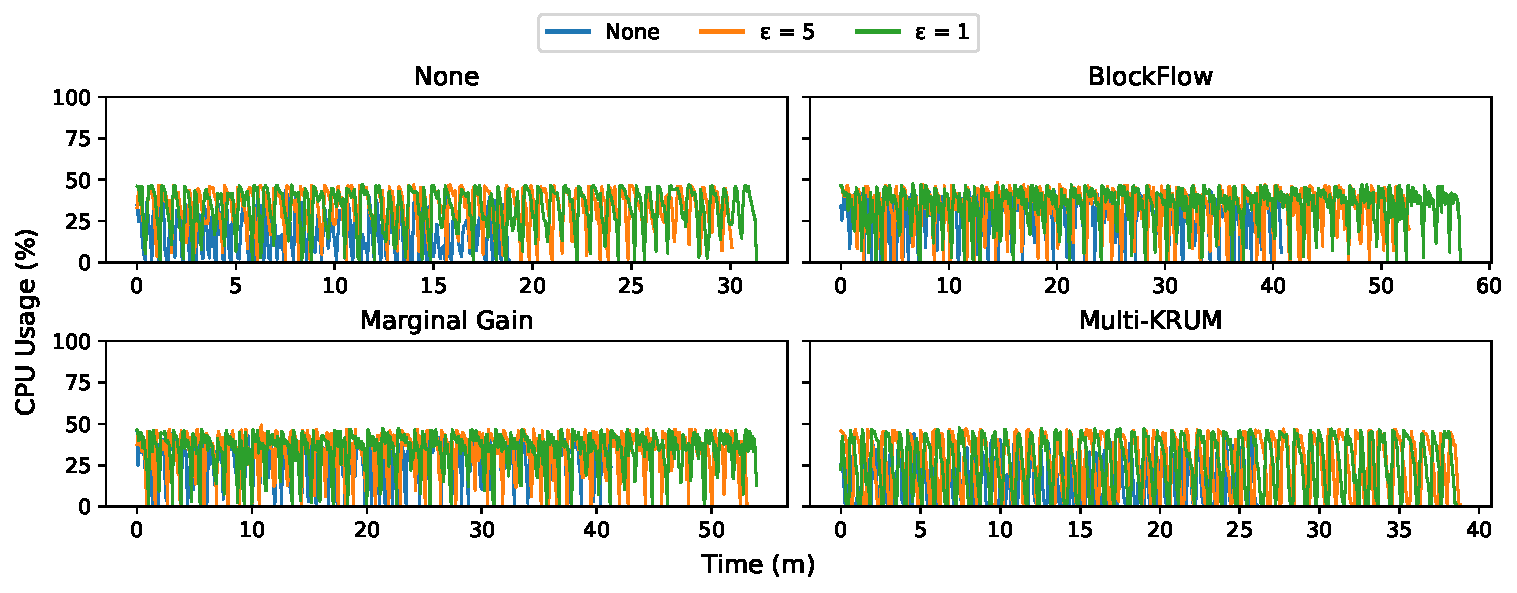
\includegraphics[width=\textwidth]{graphics/privacy/cpu_client.pdf}
    \caption{Client Process CPU Usage Per Privacy Degree}
    \label{fig:cpu_privacy_clients}
\end{figure}

\vfill

\begin{figure}[!h]
    \centering
    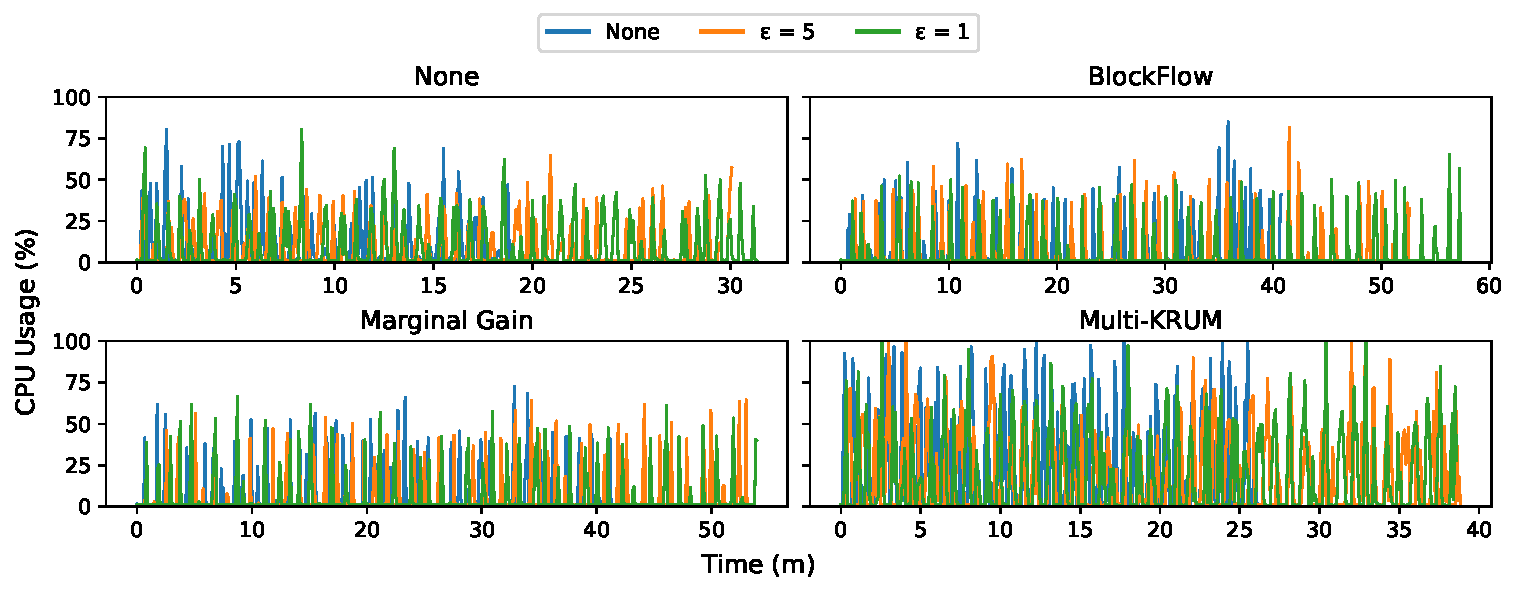
\includegraphics[width=\textwidth]{graphics/privacy/cpu_server.pdf}
    \caption{Server Process CPU Usage Per Privacy Degree}
    \label{fig:cpu_privacy_servers}
\end{figure}

\vfill

\begin{figure}[!h]
    \centering
    \includegraphics[width=\textwidth]{graphics/privacy/cpu_miner.pdf}
    \caption{Blockchain Process CPU Usage Per Privacy Degree}
    \label{fig:cpu_privacy_miners}
\end{figure}


\chapter{Proof of Concept of Vertical Blockchain-based Federated Learning}\label{chapter:vertical}
In this chapter, we provide a proof of concept of Blockchain-based Federated Learning (BFS) applied to a system with vertically partitioned data. Specifically, we aim to:

\begin{enumerate}
    \item Present design and implementation of a Vertical Blockchain-based Federated Learning system. As discussed in \Cref{related_work:other_remarks}, only one other work \cite{10.48550/arxiv.1912.04859} discusses possibilities of integration of blockchain with Vertical Federated Learning with blockchain, but it does not provide an actual design or implementation.
    
    \item Demonstrate that our framework is flexible to support additional execution flow steps and algorithms, as well as both Horizontal and Vertical Federated Learning. As explained in \Cref{eval:ml_models}, the model we use for Vertical Federated Learning requires an additional step in each round. By showing that it is trivial to add new steps to the rounds, we also show that BlockLearning is flexible.
\end{enumerate}

\section{Requirements Analysis}

As discussed in \Cref{eval:ml_models}, our Vertical Federated Learning implementation uses the Split-CNN model. This model poses different requirements on our framework when compared to a regular CNN. These requirements are as follows:

\begin{enumerate}
    \item \textit{Support different models for the clients and the servers.} As explained in \Cref{eval:ml_models}, the clients have the head model, while the servers have the tail model. This is different than the model we used for Horizontal Federated Learning, which is the same on the devices, regardless of their type.
    
    \item \textit{Support additional backpropagation confirmation phase.} After submitting the aggregations, and before terminating the round, the clients have to confirm that they backpropagated the gradient updates from the tail model to their own head models. This is related to the fact that the clients and the servers have different models.
\end{enumerate}

The second requirement can be further divided into the following functional requirements:

\begin{enumerate}
    \item Execution of backpropagation confirmation phase after aggregations submission phase.
    \item Supporting backpropagation gradient submission by the servers to the smart contract.
    \item Supporting backpropagation retrieval by the clients from the smart contract.
    \item Supporting backpropagation confirmation by the clients to the smart contract.
\end{enumerate}

The execution flow of each round when a Split-CNN model is used is illustrated in \autoref{fig:steps_vertical}. Compared to the original execution flow, depicted in \autoref{fig:blocklearning_steps}, it becomes clear that (i) the scoring phase is not used, as it is not relevant in the context of Vertical Federated Learning, and (ii) there is an additional backpropagation confirmation phase before the round is terminated. 

\begin{figure}[!ht]
    \centering
    \includegraphics[width=1\textwidth]{graphics/sequence-vertical.pdf}
    \caption{Round Execution Flow With Split-CNN Model}
    \label{fig:steps_vertical}
\end{figure}

\section{BlockLearning's Extension}

Most of the aforementioned requirements pertain the smart contract. Therefore, we first start by making the required changes to the smart contracts:

\begin{enumerate}
    \item Add a new phase, called \texttt{WaitingForBackpropagation}, to the \texttt{RoundPhase} enumeration in the \texttt{Base} contract.
    
    \item Create a new smart contract, called \texttt{VerticalSplitCNN}, which inherits the main functionality from the \texttt{Base} smart contract, and provides the additional functionalities required for the backpropagation phase.
\end{enumerate}

\autoref{fig:uml-vertical} illustrates the smart contract additions to the original design of our BlockLearning framework presented in \Cref{chapter:framework}. It is important to note that all these changes are additions, and they do not change how any existing feature behaves.

\begin{figure}[!ht]
    \centering
    \centering
    \includegraphics[width=1\textwidth]{graphics/smart-contract-uml-vertical.pdf}
    \caption{Split-CNN Smart Contracts Extension Class Diagram}
    \label{fig:uml-vertical}
\end{figure}

After creating the new smart contract, the smart contract bridge has to be extended in order to include the new smart contract functions. This extension is trivial as explained in \Cref{impl:bridge}.

The model training procedure for the Split-CNN model is slightly different from the CNN used for Horizontal Vertical Learning. For the Split-CNN, the clients submit an update with the intermediate outputs of the last layer of the head model, instead of the weights. During the aggregation phase, the servers calculate the gradients of the intermediate outputs, which are then backpropagated to the clients. To support this, we implement two new classes: \texttt{TrainerSplitCNN} and \texttt{AggregatorSplitCNN}, which implement the \texttt{trainer()} and \texttt{aggregate()} interfaces, respectively, as specified in \Cref{chapter:framework}. In addition, the \texttt{TrainerSplitCNN} class supports a new method, \texttt{backward()}, that will be called during the new backpropagation phase.

Finally, we write server and client scripts for the Vertical Federated Learning using the building blocks from the BlockLearning framework. \autoref{alg:client_loop_splitcnn} illustrates the client main loop when used with a Split-CNN model. The main differences from the original BlockLearning framework, as presented in \Cref{chapter:framework}, are that the framework does not have scoring algorithm, and that we take into account the backpropagation phase. The server main loop when used with a Split-CNN model is the same as the original server main loop except that it initializes an instance of the \texttt{AggregatorSplitCNN} class instead of the regular aggregator.

\begin{algorithm}
\caption{Client Script Main Loop for Split-CNN}\label{alg:client_loop_splitcnn}
\begin{algorithmic}
\State $T \gets $ Initialize Split-CNN Trainer
\While{True}
    \State $P \gets$ Get Phase From Smart Contract
    \If{$P$ is Waiting For Updates}
        \State Execute Training Procedure $T.train()$
    \ElsIf{$P$ is Waiting For Backpropagation}
        \State Execute Backpropagation Procedure $T.backward()$
    \EndIf
\EndWhile
\end{algorithmic}
\end{algorithm}

\section{Experiments and Results}

After extending our framework in order to support the Split-CNN model, we executed the experiments for Vertical Federated Learning in order to validate whether our implementation was successful and the Vertical BFL can be supported. The experiments were executed in the same way as the experiments for the Horizontal BFL, using BlockLearning's Testbed. The only difference is that, this time, we used the client and server scripts that we developed for the Split-CNN model.

We ran two experiments with two different number of clients: 2 and 4. The decision to use 2 clients was motivated by \cite{10.1145/3297858.3304038}, where the Split-CNN was introduced for Vertical FL without blockchain for the first time. In addition, we also performed experiments with 4 clients.

\subsection{Execution Time, Transaction Cost, and Transaction Latency}

As it can be seen from \autoref{tab:metrics_vertical}, this experiment was faster than most experiments, which is easily explained by the low number of clients. In addition, it is observed that the experiments take longer with 4 clients than with 2

Regarding the transaction latency, it can be seen that it is similar to what we have seen in previous chapters. Similarly, the transaction costs do not present significant changes as the number of clients is relatively low. However, as expected, the transaction costs are slightly higher in case of having 4 clients.

\begin{table}[!ht]
\begin{tabular}{c|c|c} \hline \hline
                                & 2             & 4             \\ \hline \hline
E2E Time (m)                    & 18.08         &	24.30       \\ \hline
Mean Round Time (s)             & 21.68         &	29.15       \\ \hline
Mean Transaction Latency (s)    & 1.482         &	1.418       \\ \hline
Mean Transaction Cost (Gas)     & 138659        &	141013      \\ \hline
\end{tabular}
\caption{Execution Time, Transaction Cost, and Transaction Latency Per Number of Clients}
\label{tab:metrics_vertical}
\end{table}

\subsection{Model Accuracy and Convergence}

\autoref{fig:accuracy_vertical} illustrates the model accuracy of our experiments as well as those of Romanini et al. \cite{10.48550/arxiv.2104.00489}, where a Split-CNN model without blockchain was used with the MNIST data set. It can be seen that model accuracy of \cite{10.48550/arxiv.2104.00489} is higher, which may be related to implementation differences, such as the Machine Learning library used, which is not known.

\begin{figure}[!ht]
    \centering
    \centering
    \includegraphics[width=0.7\textwidth]{graphics/vertical/accuracy.pdf}
    \caption{Model Accuracy Per Number of Clients}
    \label{fig:accuracy_vertical}
\end{figure}

\subsection{Communication Costs}

The communication costs, illustrated in \autoref{fig:net_vertical}, are also within the expected values.

We can observe at the client sides that there is no major difference of traffic when the number of clients increases. This can be explained by the fact that, by using a Split-CNN, each client is only required to upload its own intermediate results and downloads the gradient updates, which are similar in size.

At the servers, the costs are higher as the number of clients increases. Since the higher number of clients lead to higher number of heads in the Split-CNN model, the servers are required to download more intermediate results and to upload more gradient updates. Therefore, the network traffic at the servers increases with the number of clients.

On the blockchain, the difference of number of clients is not significant to make a significant difference on traffic, since these experiments ran with a very low number of clients.

\begin{figure}[!ht]
    \centering
    \centering
    \includegraphics[width=0.8\textwidth]{graphics/vertical/net.pdf}
    \caption{Network Traffic Per Round Per Number of Clients}
    \label{fig:net_vertical}
\end{figure}

\subsection{Computation Costs}

Computation costs, namely RAM usage and CPU usage, are depicted in \autoref{fig:ram_vertical} and \autoref{fig:cpu_vertical}, respectively.

Regarding the RAM usage, we observe that with a higher number of clients, there is a higher RAM usage on the serves and the blockchain processes. This is caused by the fact that more data is being stored in-memory due to the higher amount of intermediate results that the servers store in-memory, as well as the number of blockchain transactions in the blockchain. At the clients, however, the opposite happens. This can be explained by the fact that when there are more clients, each client has less features as per the data partitioning explained in \Cref{eval:client_sampling}.

Regarding the CPU usage, we see similar results as to the RAM usage, which are explained by the same reasons.

\section{Conclusions and Improvements}

From our experiments, we can conclude that it is possible to apply a Blockchain-based Federated Learning system to vertically partitioned data. In addition, we also showed how flexible our BlockLearning framework is and how we can add new features to it without changing the rest of the framework.

In future, it would be interesting to investigate how to make BlockLearning more generic in order to support other Vertical Federated Learning models than only Split-CNN. In addition, it would be interesting to incorporate the Private Set Intersection phase into our framework. This would allow the framework to be directly applied to cases where the clients have intersecting, but not equal, sample spaces.

\clearpage

\begin{figure}[!hpt]
    \centering
    \centering
    \includegraphics[width=0.8\textwidth]{graphics/vertical/ram.pdf}
    \caption{RAM Usage Per Number of Clients}
    \label{fig:ram_vertical}
\end{figure}

\begin{figure}[!hpb]
    \centering
    \centering
    \includegraphics[width=0.8\textwidth]{graphics/vertical/cpu.pdf}
    \caption{CPU Usage Per Number of Clients}
    \label{fig:cpu_vertical}
\end{figure}

\chapter{Conclusions and Future Directions}\label{chapter:conclusion}
BFL was initially introduced in order to facilitate desirable properties such as traceability, auditability, immutability, persistency, authentication and decentralization. Even though applying blockchain to a Federated Learning system brings these advantages, it also brings some trade-offs. Therefore, in this thesis, we explored how different algorithms used in Blockchain-based Federated Learning (BFL) systems impact the system 's performance in terms of execution time, accuracy and resource consumption. 

Our analysis of related work revealed that even though there are many works on designing BFL frameworks, a very few of them are
released to the public, or are modular. We, therefore, designed and implemented the very first open-source modular BFL framework that allows many aspects of the system to be easily customized and supports multiple architectures. By making it available to the public, it has the potential to empower future research.

\section{Observations From our Impact Analysis}\label{conclusions:evaluation}



Firstly, we analyzed the impact of different consensus algorithms, i.e., POW, POA, and QBFT. We concluded that different consensus algorithms play a large role in the energy consumption. In terms of computation costs, the PoW algorithm presented the highest consumption, while QBFT and PoA presented lower consumption. Regarding communication costs, QBFT had up to three times more network traffic compared to its counterparts. Consequently, we concluded that the PoA algorithm is the most cost-efficient algorithm. However, it is criticized for the degree of decentralization it provides due to the way the validator nodes are chosen. Therefore, we concluded that there is a \textit{trade-off between the degree of decentralization and the energy costs of the consensus algorithm}.

In third place, we analyzed the impact of different participant selection algorithms, which revealed to be similar in terms of energy consumption. However, randomly selecting participants revealed to be fairer and provide more stable accuracy convergence, as it gives every client an equal chance of participating in a round as long as the randomness is provided by a uniform distribution.

In fourth place, the scoring algorithms were analyzed. The scoring algorithms are required in order to filter worse contributions and prevent attacks, such as poisoning and plagiarism attacks. In addition, the scores are often used in order to give each client a reward for their contribution in order to incentive the client to participate. By adding a scoring algorithm, the execution time will increase up to twice as much, depending on whether the scoring algorithm is executed at the clients or the servers. There is a clear \textit{trade-off between the different kinds of scoring algorithms and the execution time and energy consumption, at both the clients and servers}.

In fifth place, we analyzed the impact of the number of clients and the privacy degrees on each scoring algorithm. We concluded that Marginal Gain is the most resilient to both, but also the one that consumes the most energy at the clients. Multi-KRUM revealed to be a good alternative in case the clients are low-powered devices and their communication and computations should be minimized. Finally, BlockFlow revealed to perform the worst in all aspects. We can conclude that there is a \textit{trade-off between accuracy and resiliency, and the resource consumption at the clients}.

In sixth, we provided a proof of concept of how Vertical Federated Learning can be applied to a BFL system.

\section{Looking Back to the Main Research Question}\label{conclusions:general}

The main research question of this thesis was \textit{"What is the impact of different consensus, participant selection and scoring algorithms in a Blockchain-based Federated Learning system on execution time, convergence and accuracy, as well as communication and computation costs?"}. 

Overall, our extensive experiments answered this by revealing that the addition of the blockchain, namely Ethereum, has impacts both in terms of execution time and resource usage. The average transaction latency we observed was around $1.5$ seconds. In each round, there are at least $C+S+2$ transactions, where $C$ and $S$ are the number of clients, and servers, respectively. Even though the clients and the servers execute their process in parallel, the transactions latency add up, increasing the execution time. Therefore, we conclude there is a general \textit{trade-off between the benefits of the blockchain and the execution time}.

After all, when adding the blockchain, we are adding a new layer to a system that would otherwise have a single centralized server. In order to achieve decentralization, we require more than one machine to replace the central server. Moreover, this machines must reach a consensus in terms of storage and execution. The costs of getting a system that provides traceability, auditability, immutability, persistency, authentication and decentralization are translated in higher energy costs and execution times.

% It is important (maybe not as we mentioned this before) to refer that, as mentioned previously in this work, there are other architectures. For example, in some architectures the clients are also the servers and the blockchain nodes. That is, the same machines execute all of the processing. However, this would not be feasible in an IoT system, or any other system where low-powered devices are the norm.


\section{Future Work}\label{conclusions:future_work}

Firstly, it would be interesting to build a GUI for BlockLearning that, not only allows to submit new training requests, but also provides an interactive way of visualizing the steps of the process, as well as transactions and communications.

Secondly, it would be worth investigating more methods of scoring algorithms that do not require evaluating the model with them. Both Marginal Gain and BlockFlow require that the model is evaluated by the clients, which consumes more resources and takes some time. On the other hand, Multi-KRUM scores updates by comparing the weight values directly. It would be interesting to see if such a method could be applied on the clients and if would bring the resource consumption down at the clients.

Finally, research in Blockchain-based Vertical Federated Learning should continue. Vertical Federated Learning solves a unique problem where multiple parties have different features on the same samples. The proof of concept provided in this work uses a very specific model that would not be applicable to many use cases. Therefore, more work into different types of model and architectures is required in order to understand the full potential.


\bibliographystyle{acm}
\bibliography{literature}

% \appendix 
% \addcontentsline{toc}{chapter}{Appendix}

\end{document}